%% Tipo di documento. L'uso di twoside implica che i capitoli inizino sempre con la prima pagina a sinistra, eventualmente lasciando una pagina vuota nel capitolo precedente. Se questa cosa è fastidiosa, è possibile rimuoverlo. 
\documentclass[a4paper, openright]{report}

% Dimensione dei margini
\usepackage[a4paper,top=2cm,bottom=2cm,left=2cm,right=2cm]{geometry} 
% Dimensione del font
\usepackage[fontsize=12pt]{scrextend}
% Lingua del testo
\usepackage[english]{babel}
% Lingua per la bibliografia
\usepackage[fixlanguage]{babelbib}
% Codifica del testo
\usepackage[utf8]{inputenc} 
% Encoding del testo
\usepackage[T1]{fontenc}
% Per ruotare le immagini
\usepackage{rotating}
% Per modificare l'header delle pagine 
\usepackage{fancyhdr}               

% Librerie matematiche
\usepackage{amssymb}
\usepackage{amsmath}
\usepackage{amsthm}         

% Uso delle immagini
\usepackage{graphicx}
% Uso dei colori
\usepackage[dvipsnames]{xcolor}         
% Uso dei listing per il codice
\usepackage{listings}          
% Per inserire gli hyperlinks tra i vari elementi del testo 
\usepackage{hyperref}     
% Diversi tipi di sottolineature
\usepackage[normalem]{ulem}


\usepackage{blindtext}
\usepackage{titlesec}
\usepackage{ragged2e}
\usepackage{import}
\graphicspath{{./../../../}}

\definecolor{delim}{RGB}{20,105,176}
\definecolor{numb}{RGB}{106, 109, 32}
\definecolor{string}{rgb}{0.64,0.08,0.08}

\lstdefinelanguage{json}{
    numbers=left,
    numberstyle=\small,
    frame=single,
    rulecolor=\color{black},
    showspaces=false,
    showtabs=false,
    breaklines=true,
    postbreak=\raisebox{0ex}[0ex][0ex]{\ensuremath{\color{gray}\hookrightarrow\space}},
    breakatwhitespace=true,
    basicstyle=\ttfamily\small,
    upquote=true,
    morestring=[b]",
    stringstyle=\color{string},
    literate=
     *{0}{{{\color{numb}0}}}{1}
      {1}{{{\color{numb}1}}}{1}
      {2}{{{\color{numb}2}}}{1}
      {3}{{{\color{numb}3}}}{1}
      {4}{{{\color{numb}4}}}{1}
      {5}{{{\color{numb}5}}}{1}
      {6}{{{\color{numb}6}}}{1}
      {7}{{{\color{numb}7}}}{1}
      {8}{{{\color{numb}8}}}{1}
      {9}{{{\color{numb}9}}}{1}
      {\{}{{{\color{delim}{\{}}}}{1}
      {\}}{{{\color{delim}{\}}}}}{1}
      {[}{{{\color{delim}{[}}}}{1}
      {]}{{{\color{delim}{]}}}}{1},
}
\usepackage{xr}
\externaldocument{./appendix}
\newcommand{\cref}[1]{(Appendix \ref{#1})}


% Stile del codice
\lstdefinestyle{codeStyle}{
    % Colore dei commenti
    commentstyle=\color{teal},
    % Colore delle keyword
    keywordstyle=\color{Magenta},
    % Stile dei numeri di riga
    numberstyle=\tiny\color{gray},
    % Colore delle stringhe
    stringstyle=\color{violet},
    % Dimensione e stile del testo
    basicstyle=\ttfamily\footnotesize,
    % newline solo ai whitespaces
    breakatwhitespace=false,     
    % newline si/no
    breaklines=true,                 
    % Posizione della caption, top/bottom 
    captionpos=b,                    
    % Mantiene gli spazi nel codice, utile per l'indentazione
    keepspaces=true,                 
    % Dove visualizzare i numeri di linea
    numbers=left,                    
    % Distanza tra i numeri di linea
    numbersep=5pt,                  
    % Mostra gli spazi bianchi o meno
    showspaces=false,                
    % Mostra gli spazi bianchi nelle stringhe
    showstringspaces=false,
    % Mostra i tab
    showtabs=false,
    % Dimensione dei tab
    tabsize=2
} \lstset{style=codeStyle}


\newcounter{alphasect}
\def\alphainsection{0}

\let\oldsection=\section
\def\section{%
  \ifnum\alphainsection=1%
    \addtocounter{alphasect}{1}
  \fi%
\oldsection}%

\renewcommand\thesection{%
  \ifnum\alphainsection=1% 
    \Alph{alphasect}
  \else%
    \arabic{section}
  \fi%
}%

\newenvironment{alphasection}{%
  \ifnum\alphainsection=1%
    \errhelp={Let other blocks end at the beginning of the next block.}
    \errmessage{Nested Alpha section not allowed}
  \fi%
  \setcounter{alphasect}{0}
  \def\alphainsection{1}
}{%
  \setcounter{alphasect}{0}
  \def\alphainsection{0}
}



% Taken from Lena Herrmann at 
% http://lenaherrmann.net/2010/05/20/javascript-syntax-highlighting-in-the-latex-listings-package
\lstdefinelanguage{JavaScript}{
  keywords={typeof, new, true, false, catch, function, return, null, catch, switch, var, if, in, while, do, else, case, break},
  keywordstyle=\color{blue}\bfseries,
  ndkeywords={class, export, boolean, throw, implements, import, this},
  ndkeywordstyle=\color{darkgray}\bfseries,
  identifierstyle=\color{black},
  sensitive=false,
  comment=[l]{//},
  morecomment=[s]{/*}{*/},
  commentstyle=\color{purple}\ttfamily,
  stringstyle=\color{red}\ttfamily,
  morestring=[b]',
  morestring=[b]"
}

\lstset{
   language=JavaScript,
   backgroundcolor=\color{lightgray},
   extendedchars=true,
   basicstyle=\footnotesize\ttfamily,
   showstringspaces=false,
   showspaces=false,
   numbers=left,
   numberstyle=\footnotesize,
   numbersep=9pt,
   tabsize=2,
   breaklines=true,
   showtabs=false,
   captionpos=b
}


%\begin{document}

\chapter{Instruction Manual}

The application is accessible through a web browser and doesn't require an authentication to perform some basic navigation and scrolling of movies and reviews. To leave a review under a movie, follow top critics and receive personalized information, a user must log-in or sign-up to the service. Some notable and certified users may be registered by an administrator as a \textit{Top Critic} which can be followed by other users and whose reviews are highlighted under a movie

\section{Greeting Page}

\hspace{-45pt}
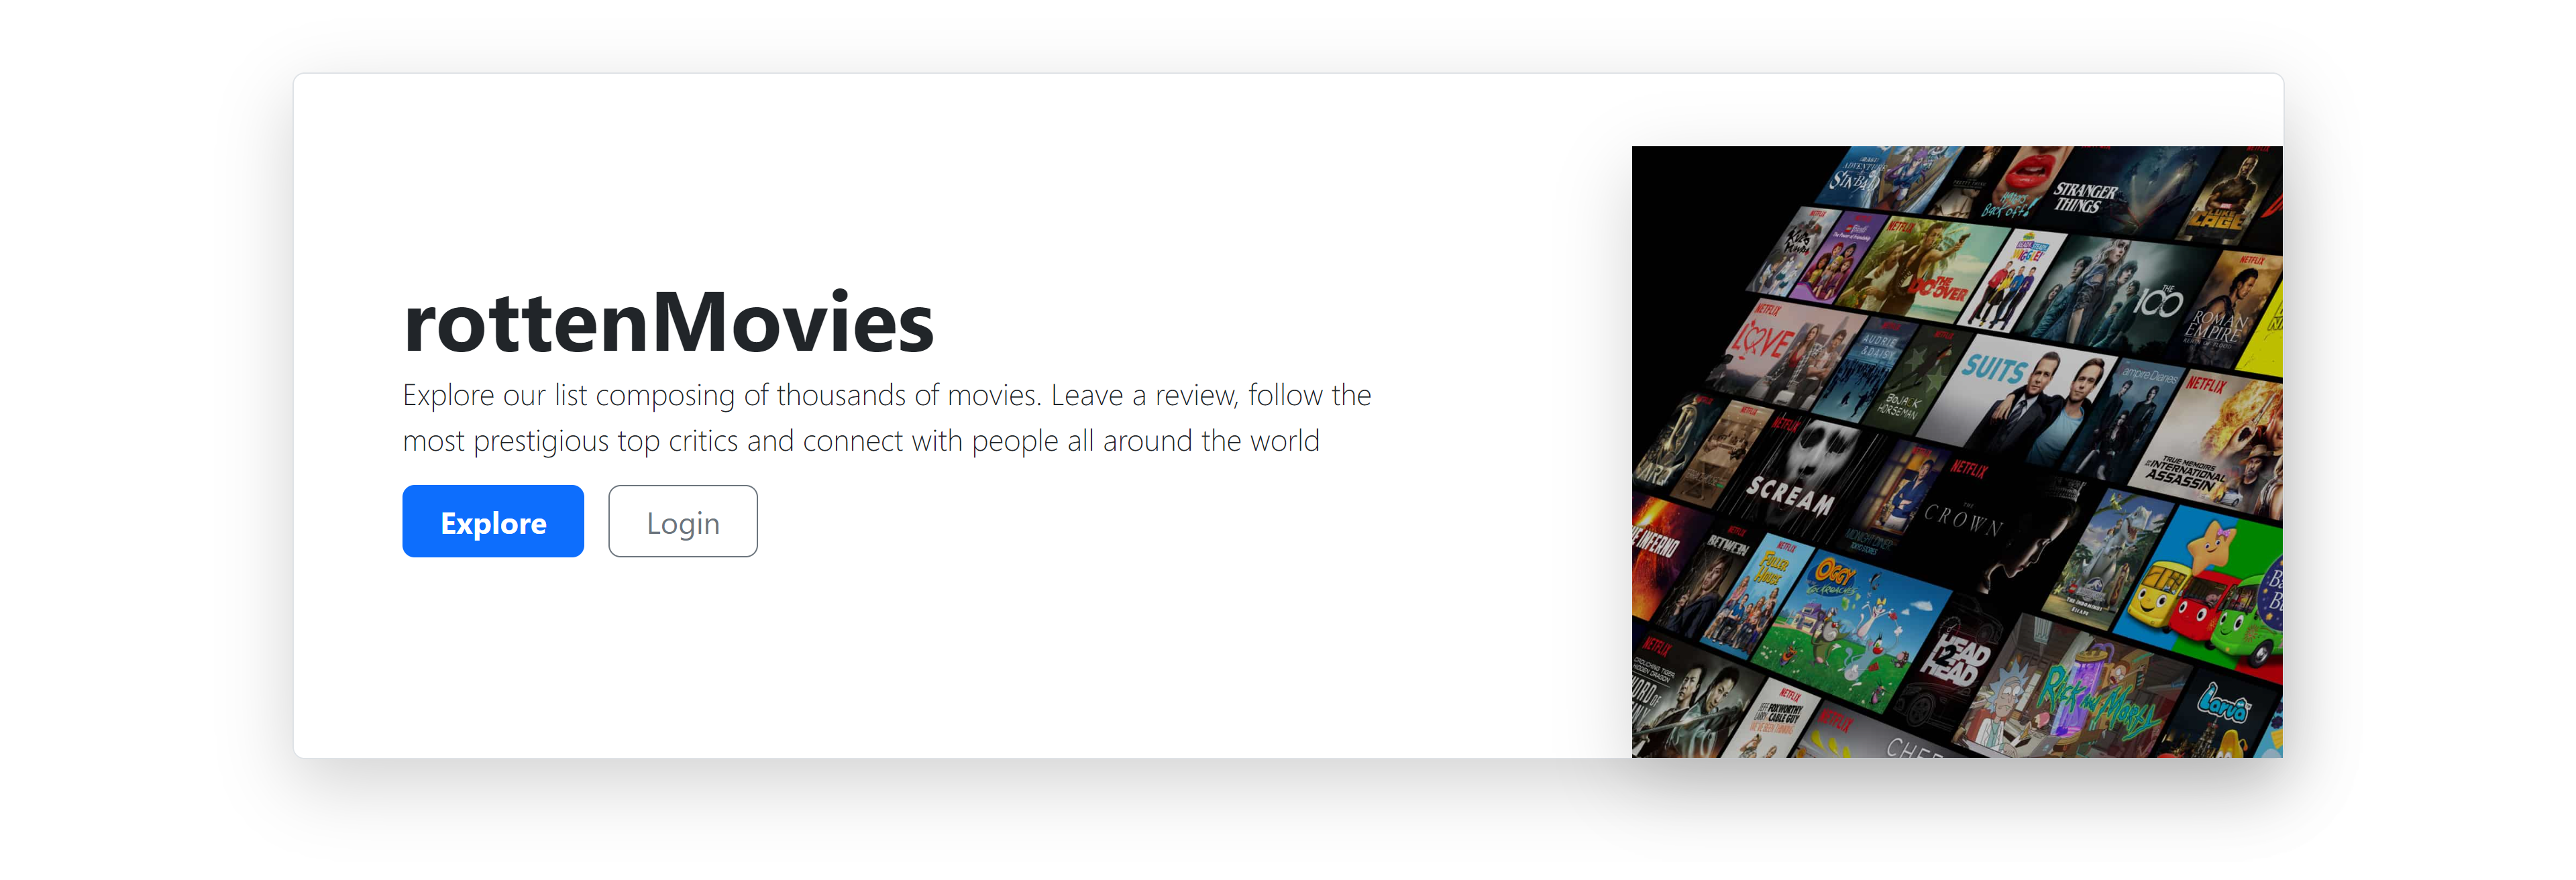
\includegraphics[scale=0.45]{../../../images/user_manual/index.png} 


The landing page presents the option to jump directly to the main page for exploring movies and incites the new user to login or sign-up to the application.
\begin{center}
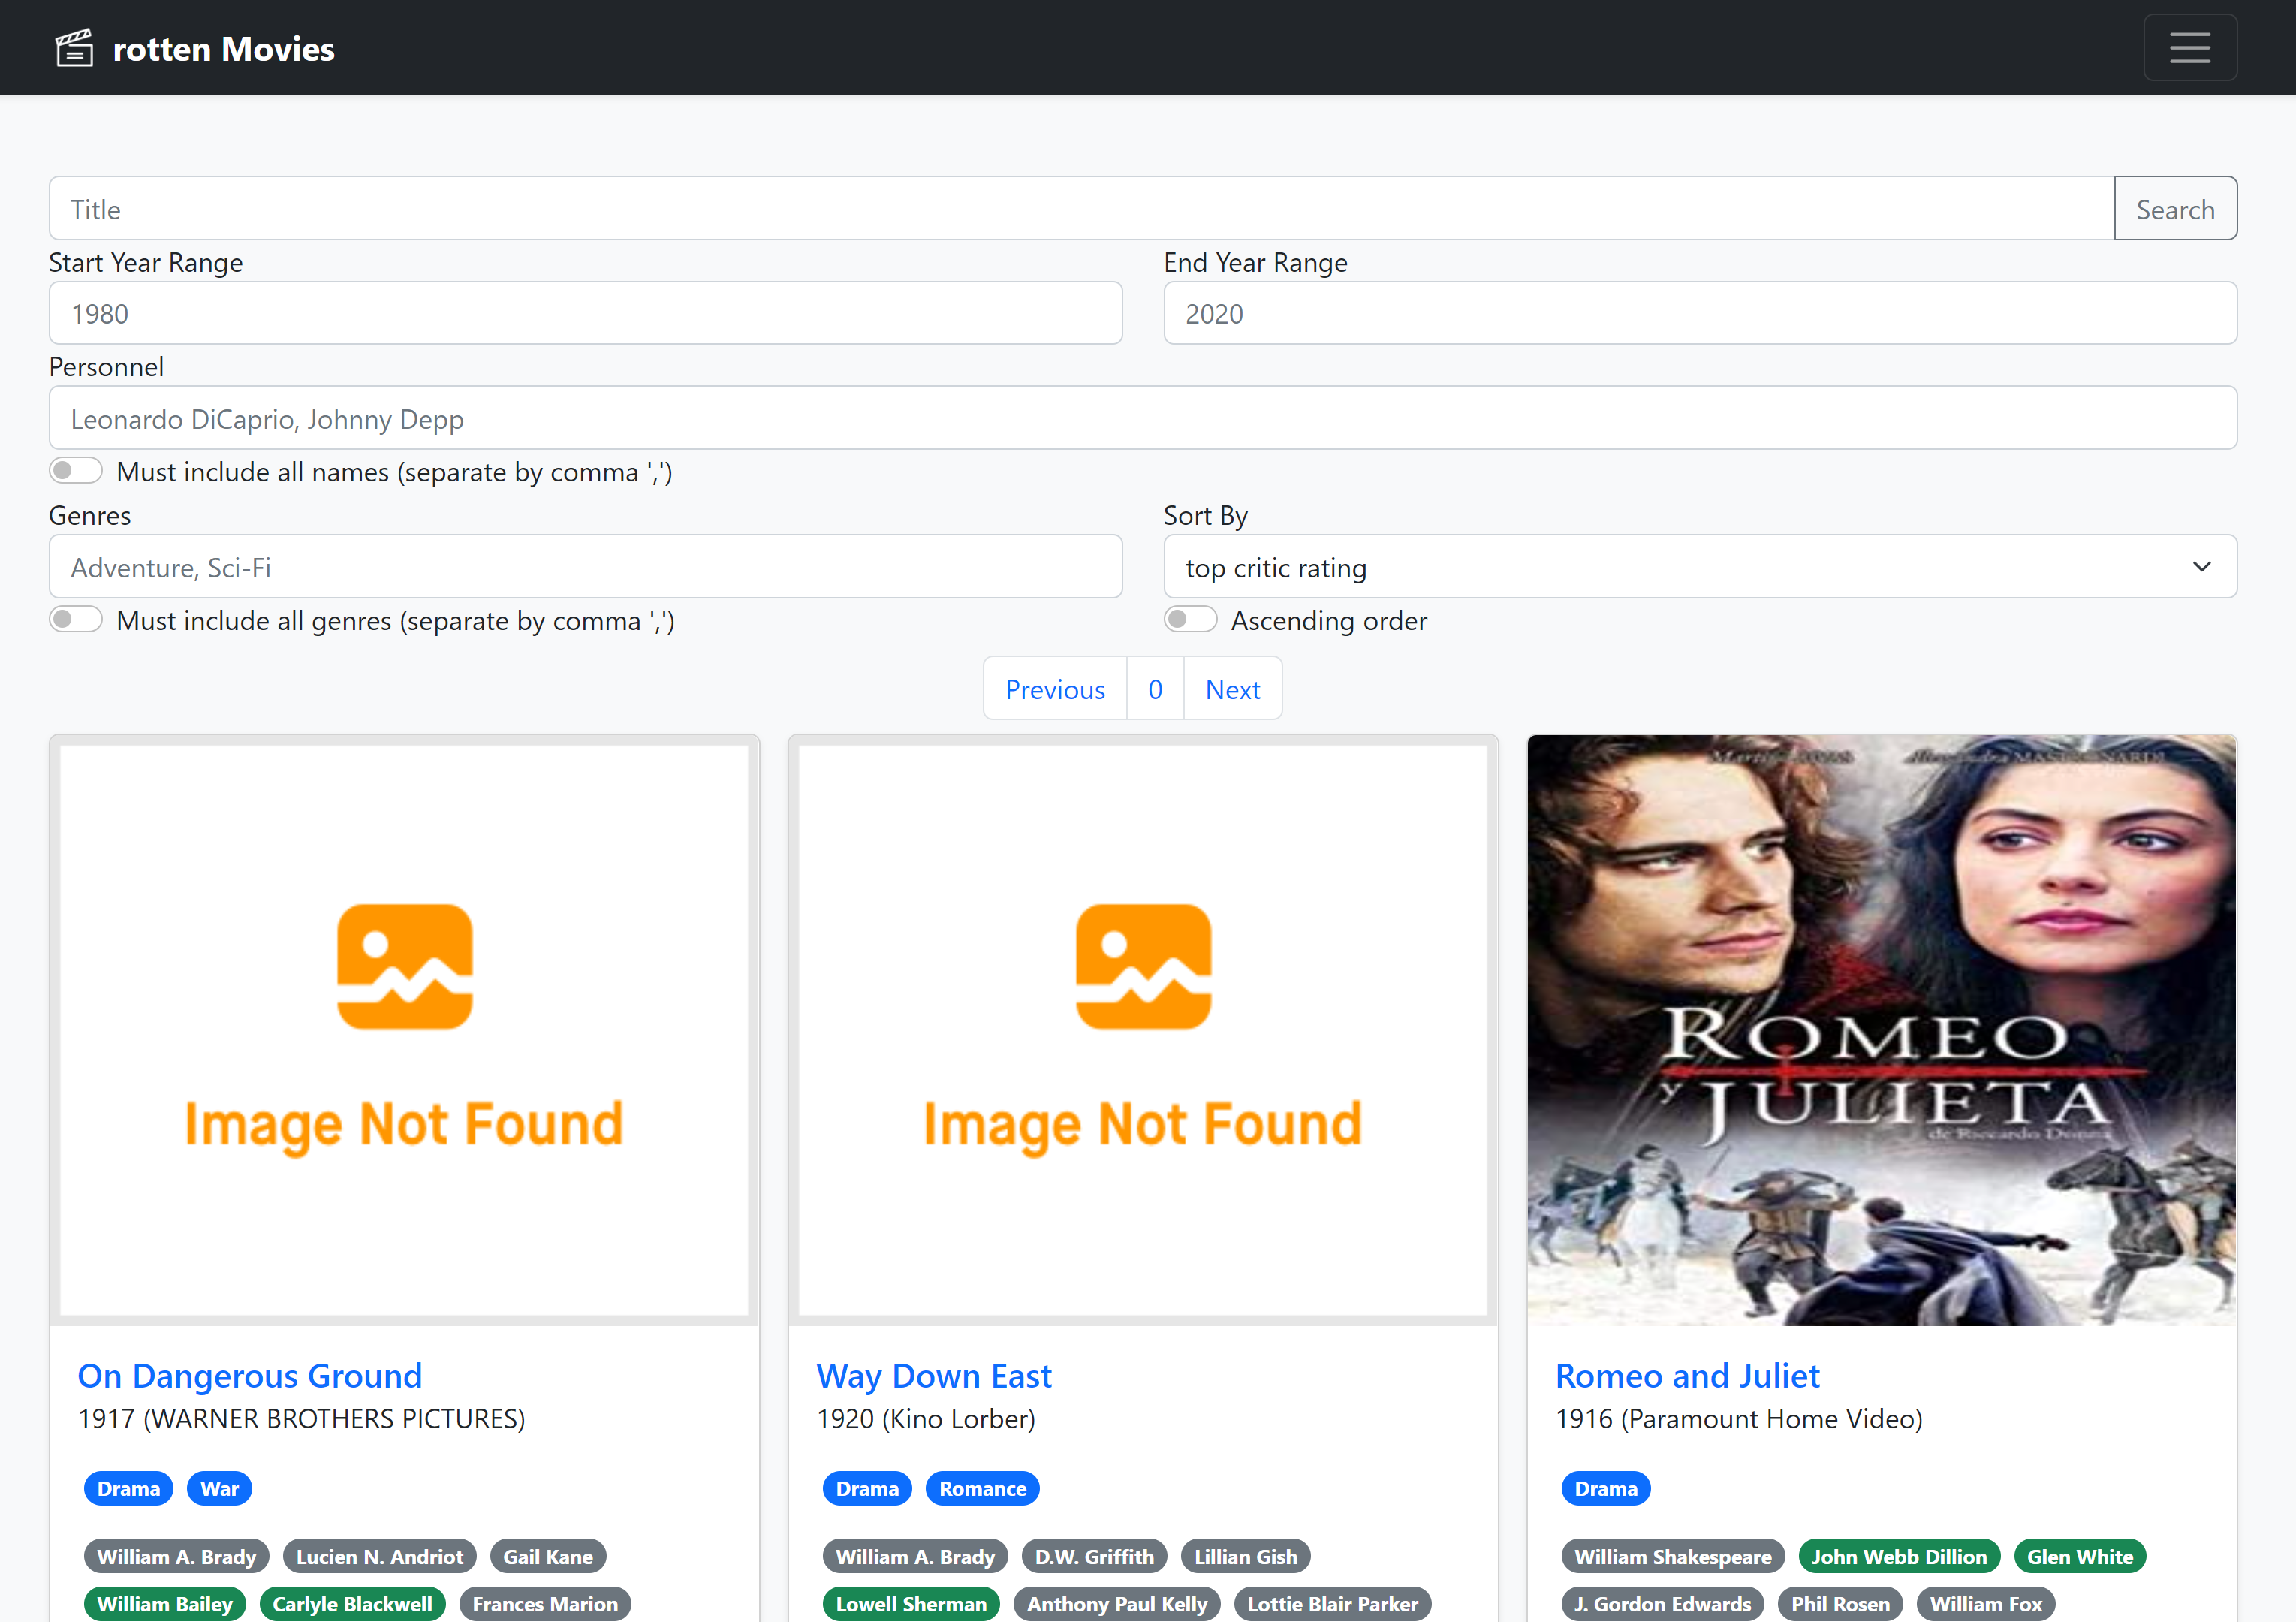
\includegraphics[scale=0.45]{../../../images/user_manual/search.png} 
\end{center}
\vspace{5pt}

The exploring page offers multiple options to filter between all movies inside the database
\begin{center}
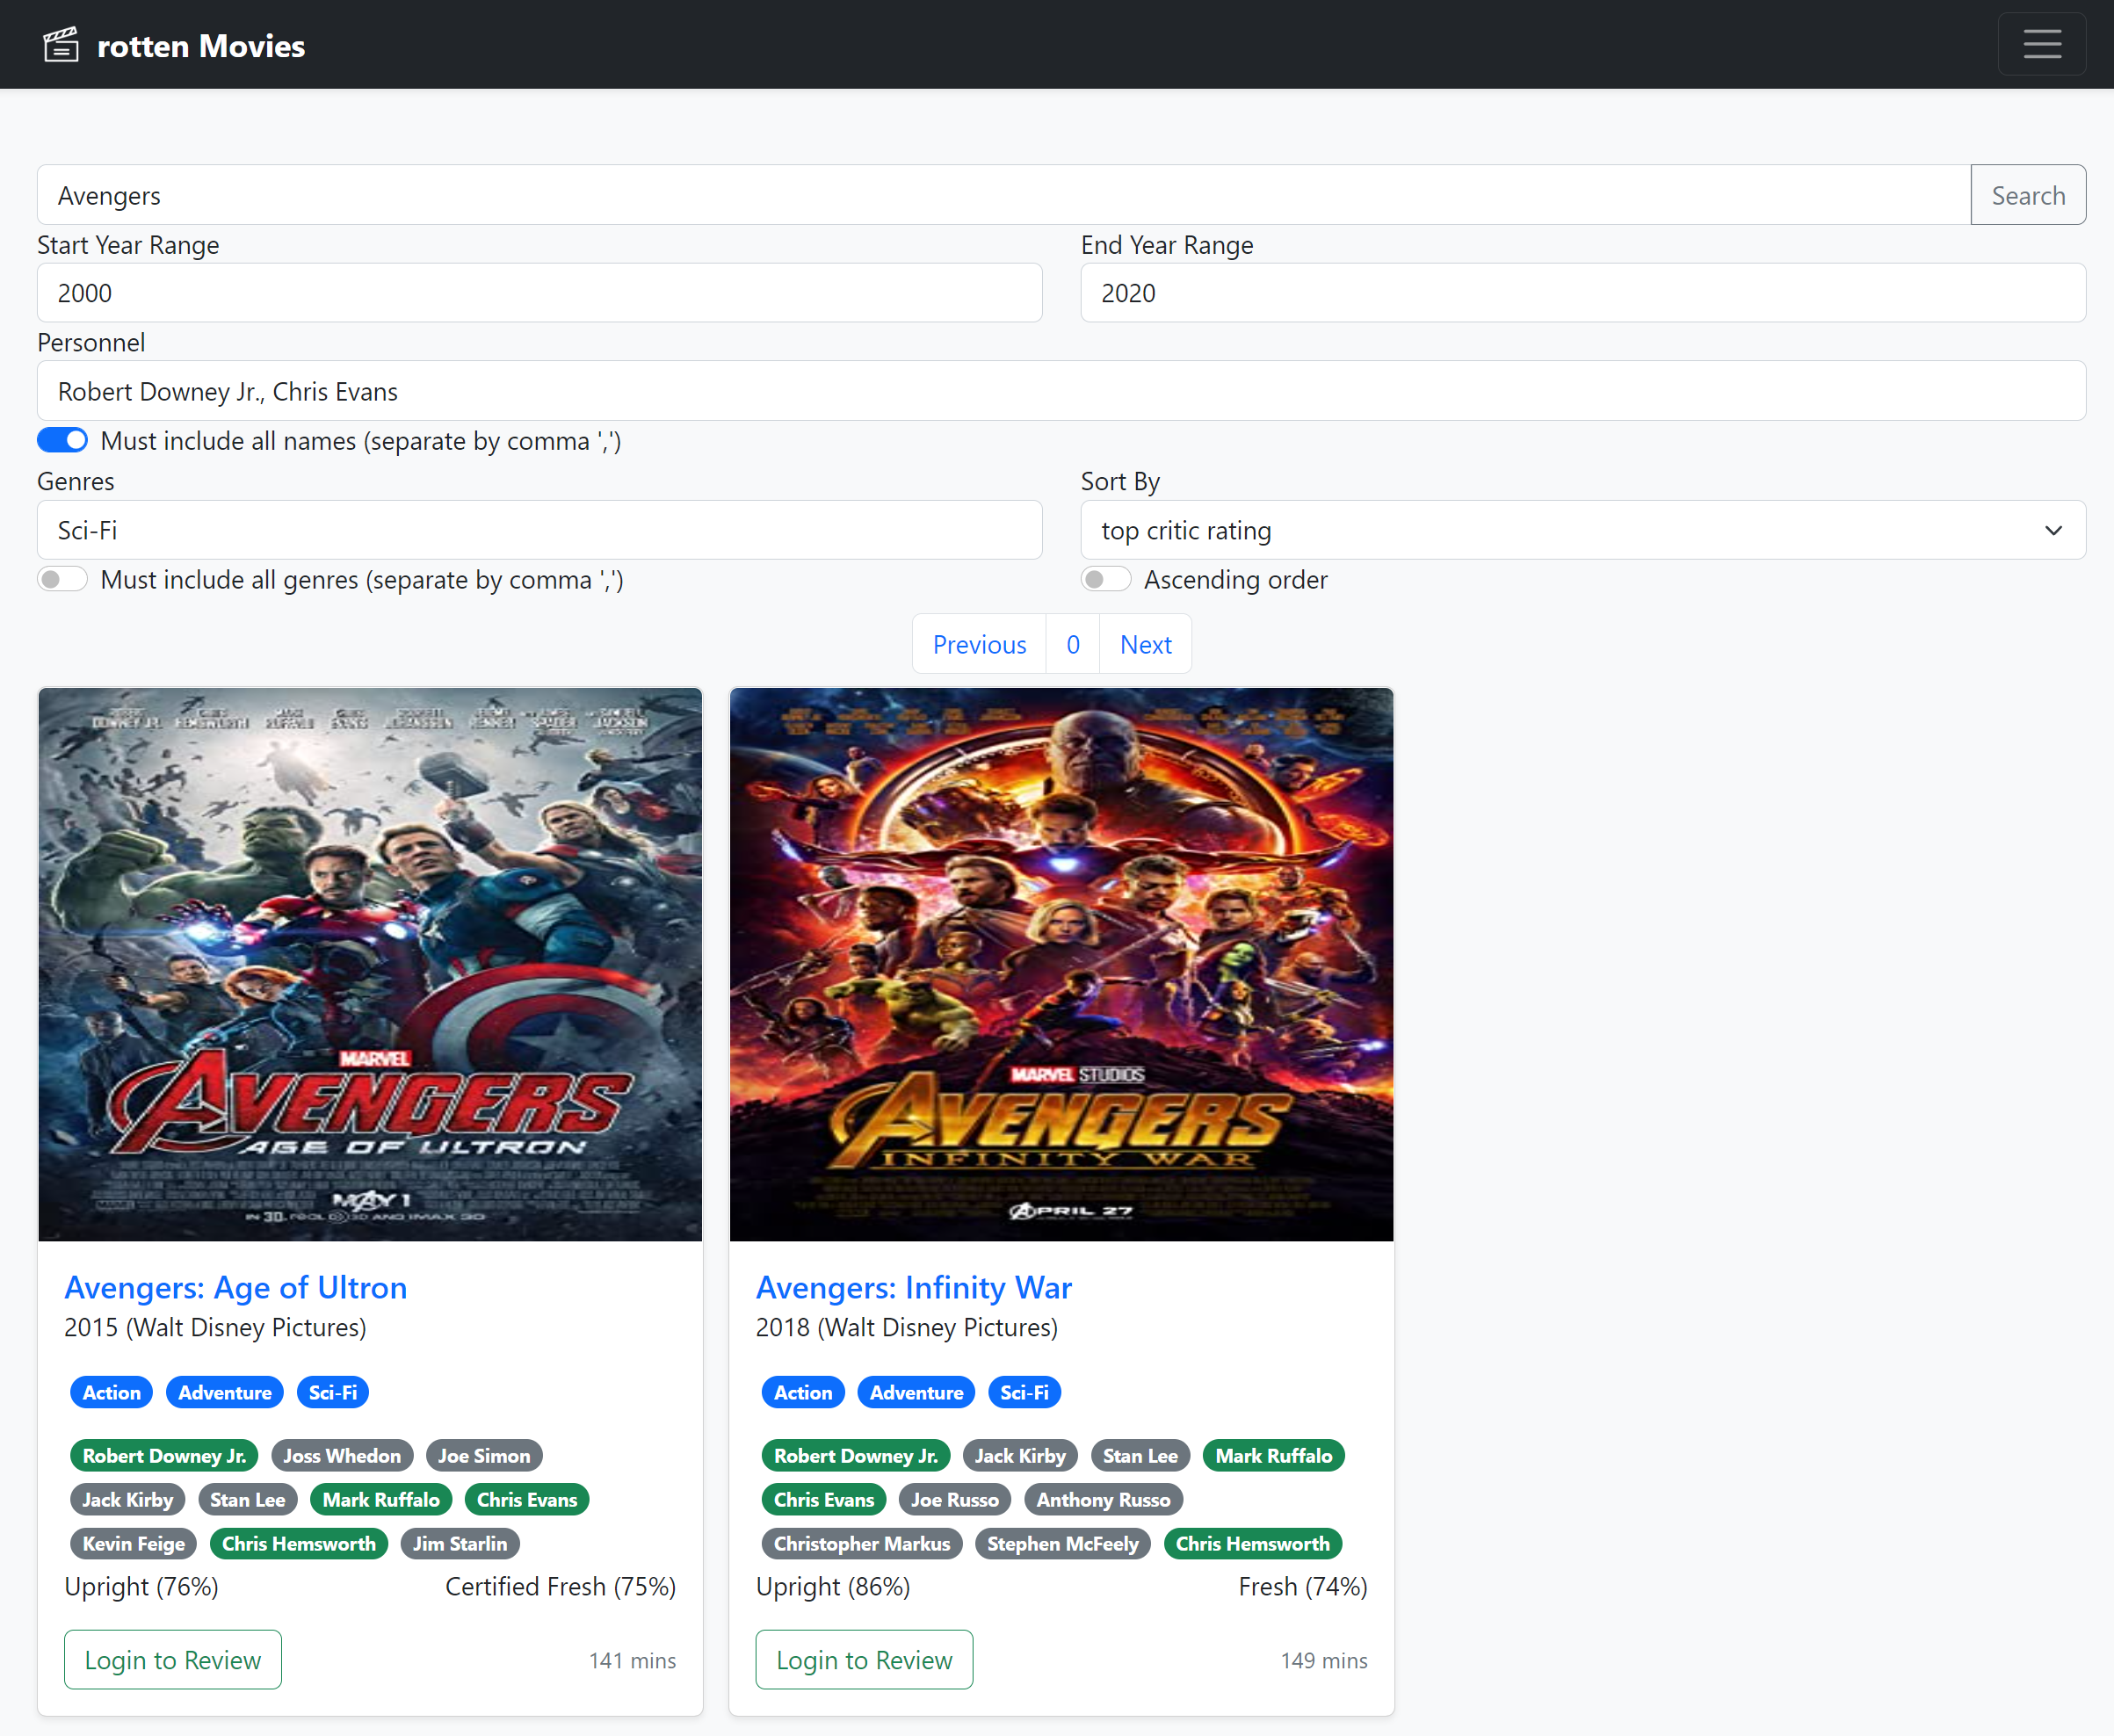
\includegraphics[scale=0.45]{../../../images/user_manual/search_query.png} 
\end{center}
\vspace{5pt}

It is possible to search by 
\begin{itemize}
\item a string contained in the title
\item a range of year in which the movie has been produced
\item people that worked on the film. It is possible to build a list of names by employing a comma (,) and stating if the movie must include all names or at least one of them
\item genres. It is possible to build a list of genres by employing a comma (,) and stating if the movie must include all genres or at least one of them
\end{itemize}

The available sorting options are
\begin{itemize}
\item by top critic rating (the default)
\item by user critic rating
\item alphabetical order
\item by date of production
\end{itemize}
and the user can opt for an ascending or descending sort.

At any point the user can click on the pills of genres or crew members to perform a search with that value.

If a user isn't logged-in, the button under a movie says 'Login to Review' and brings to the login page. Otherwise it becomes 'Review' and clicking on it allows the quick creation or editing of the review for that movie.
\begin{center}
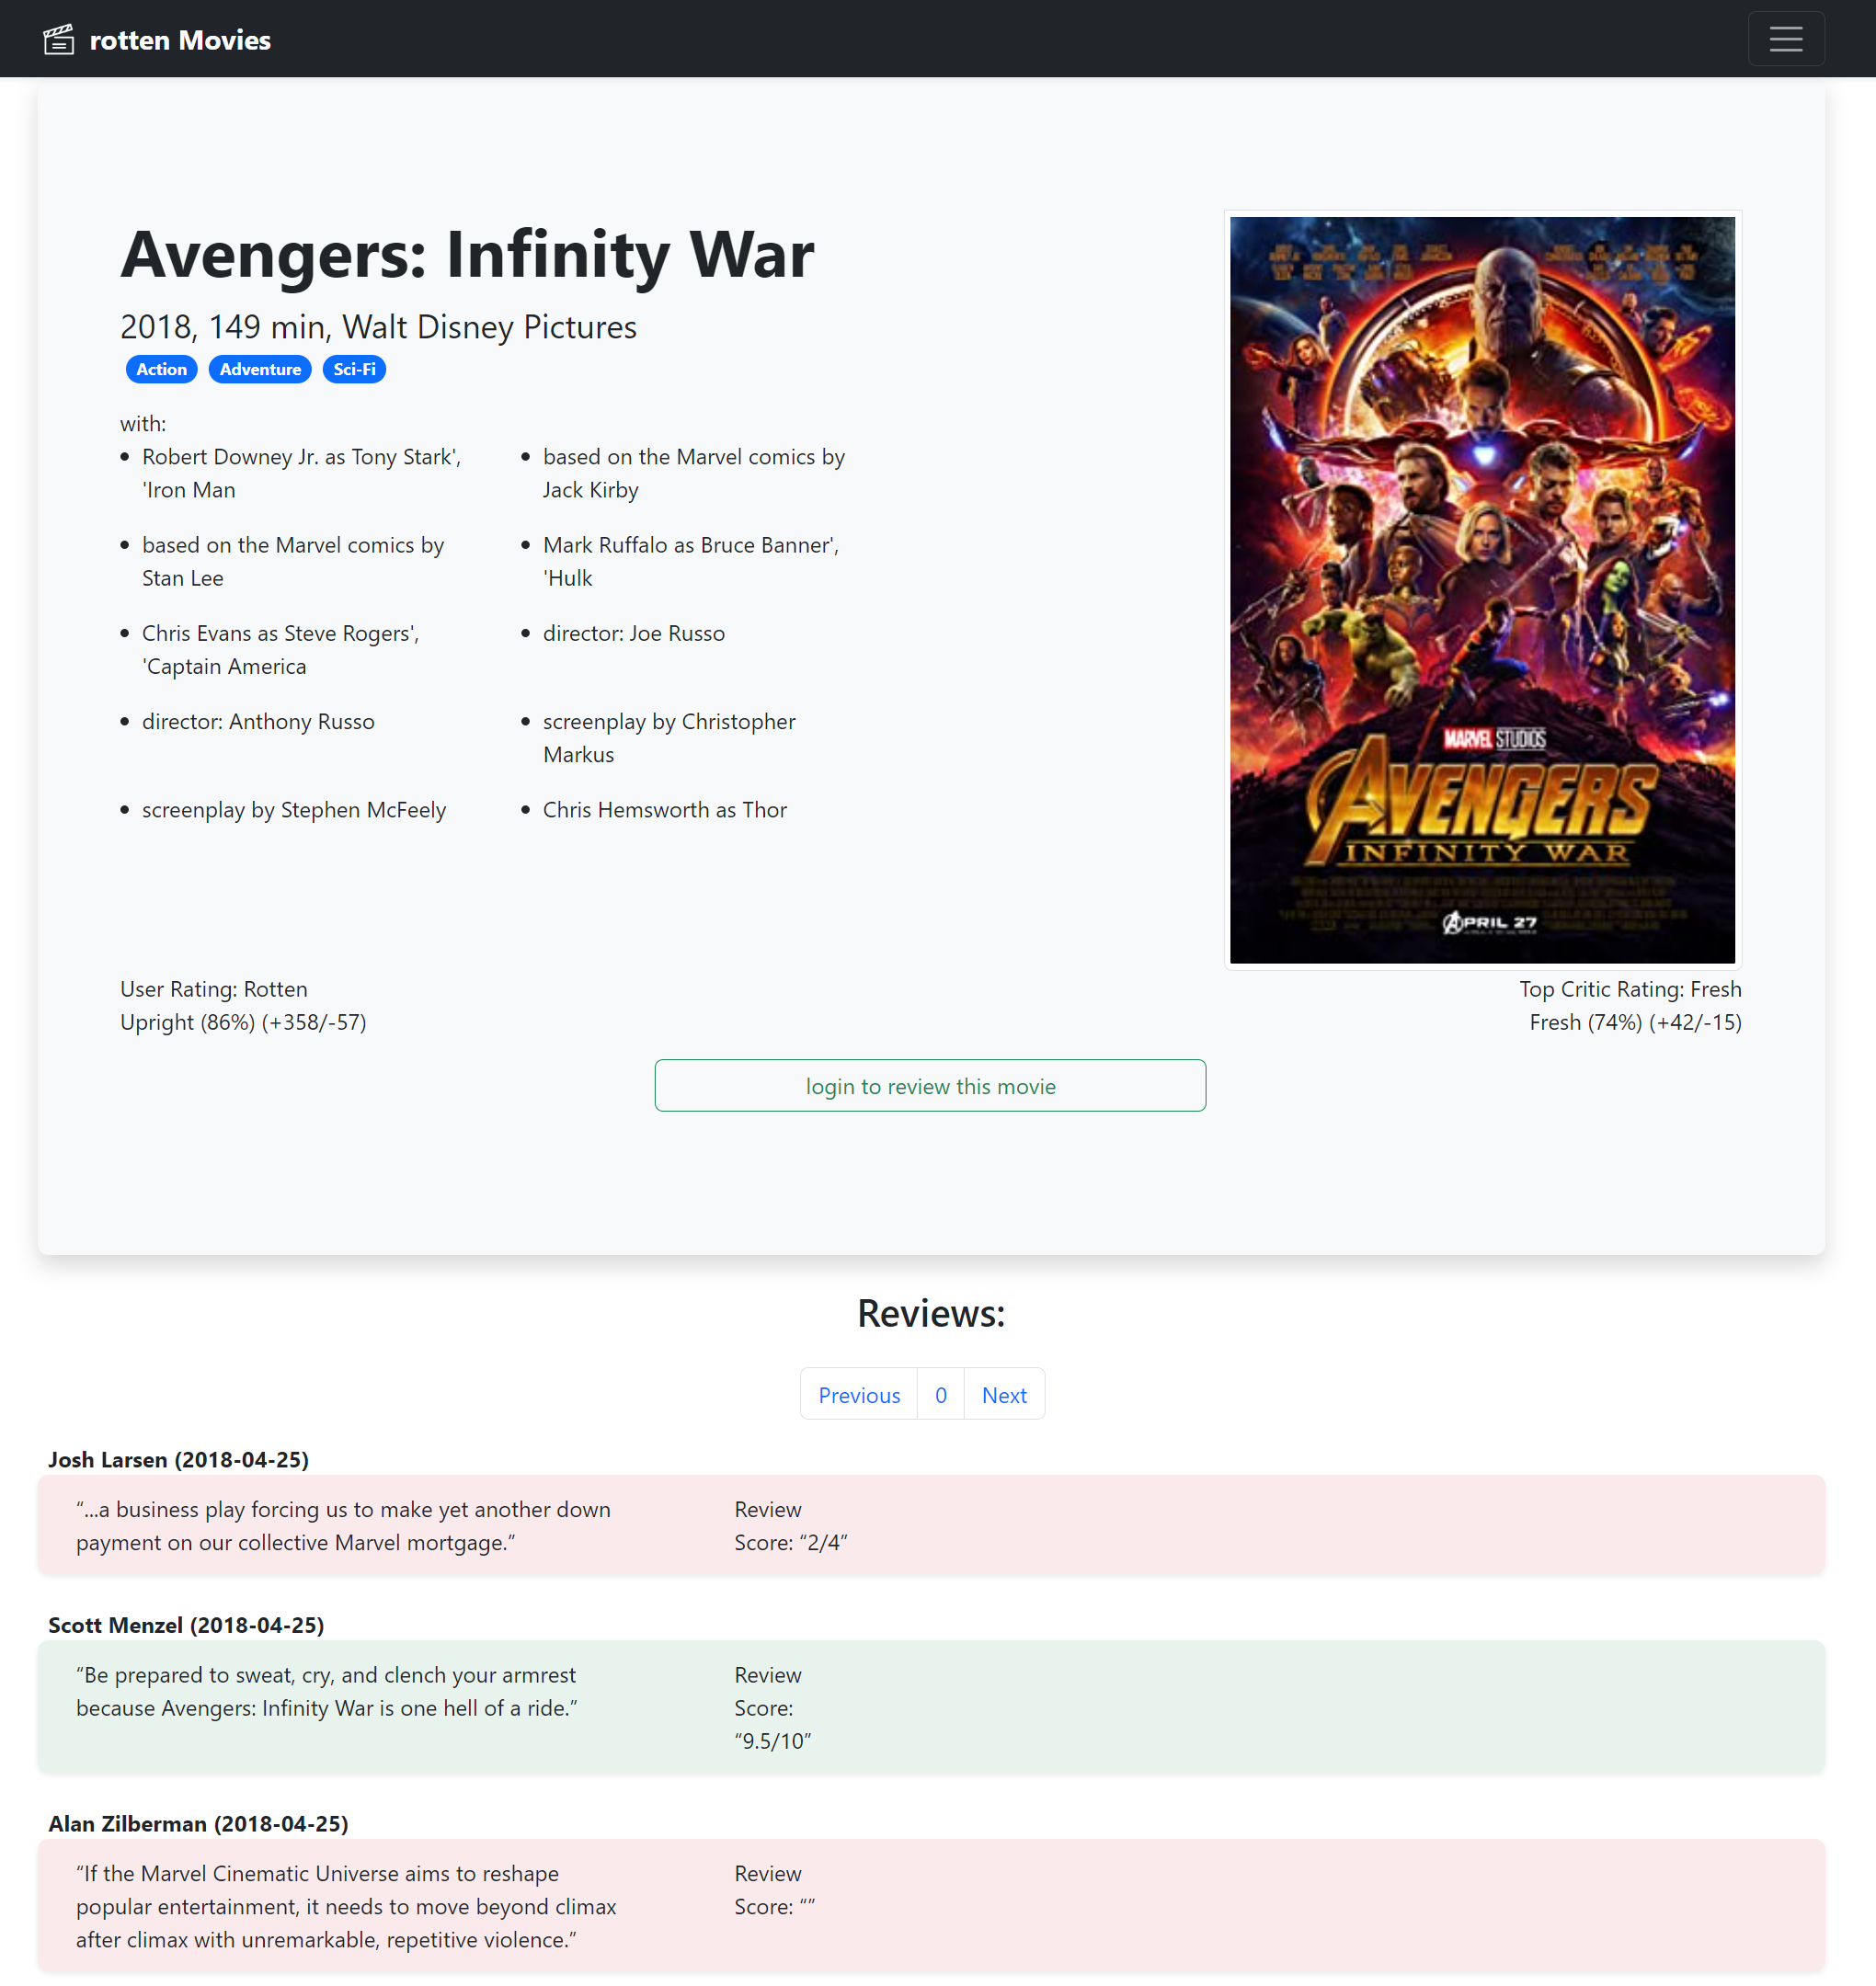
\includegraphics[scale=0.45]{../../../images/user_manual/movie_page.png} 
\end{center}
\vspace{5pt}

Selecting a movie allows to see a full description of it
\begin{center}
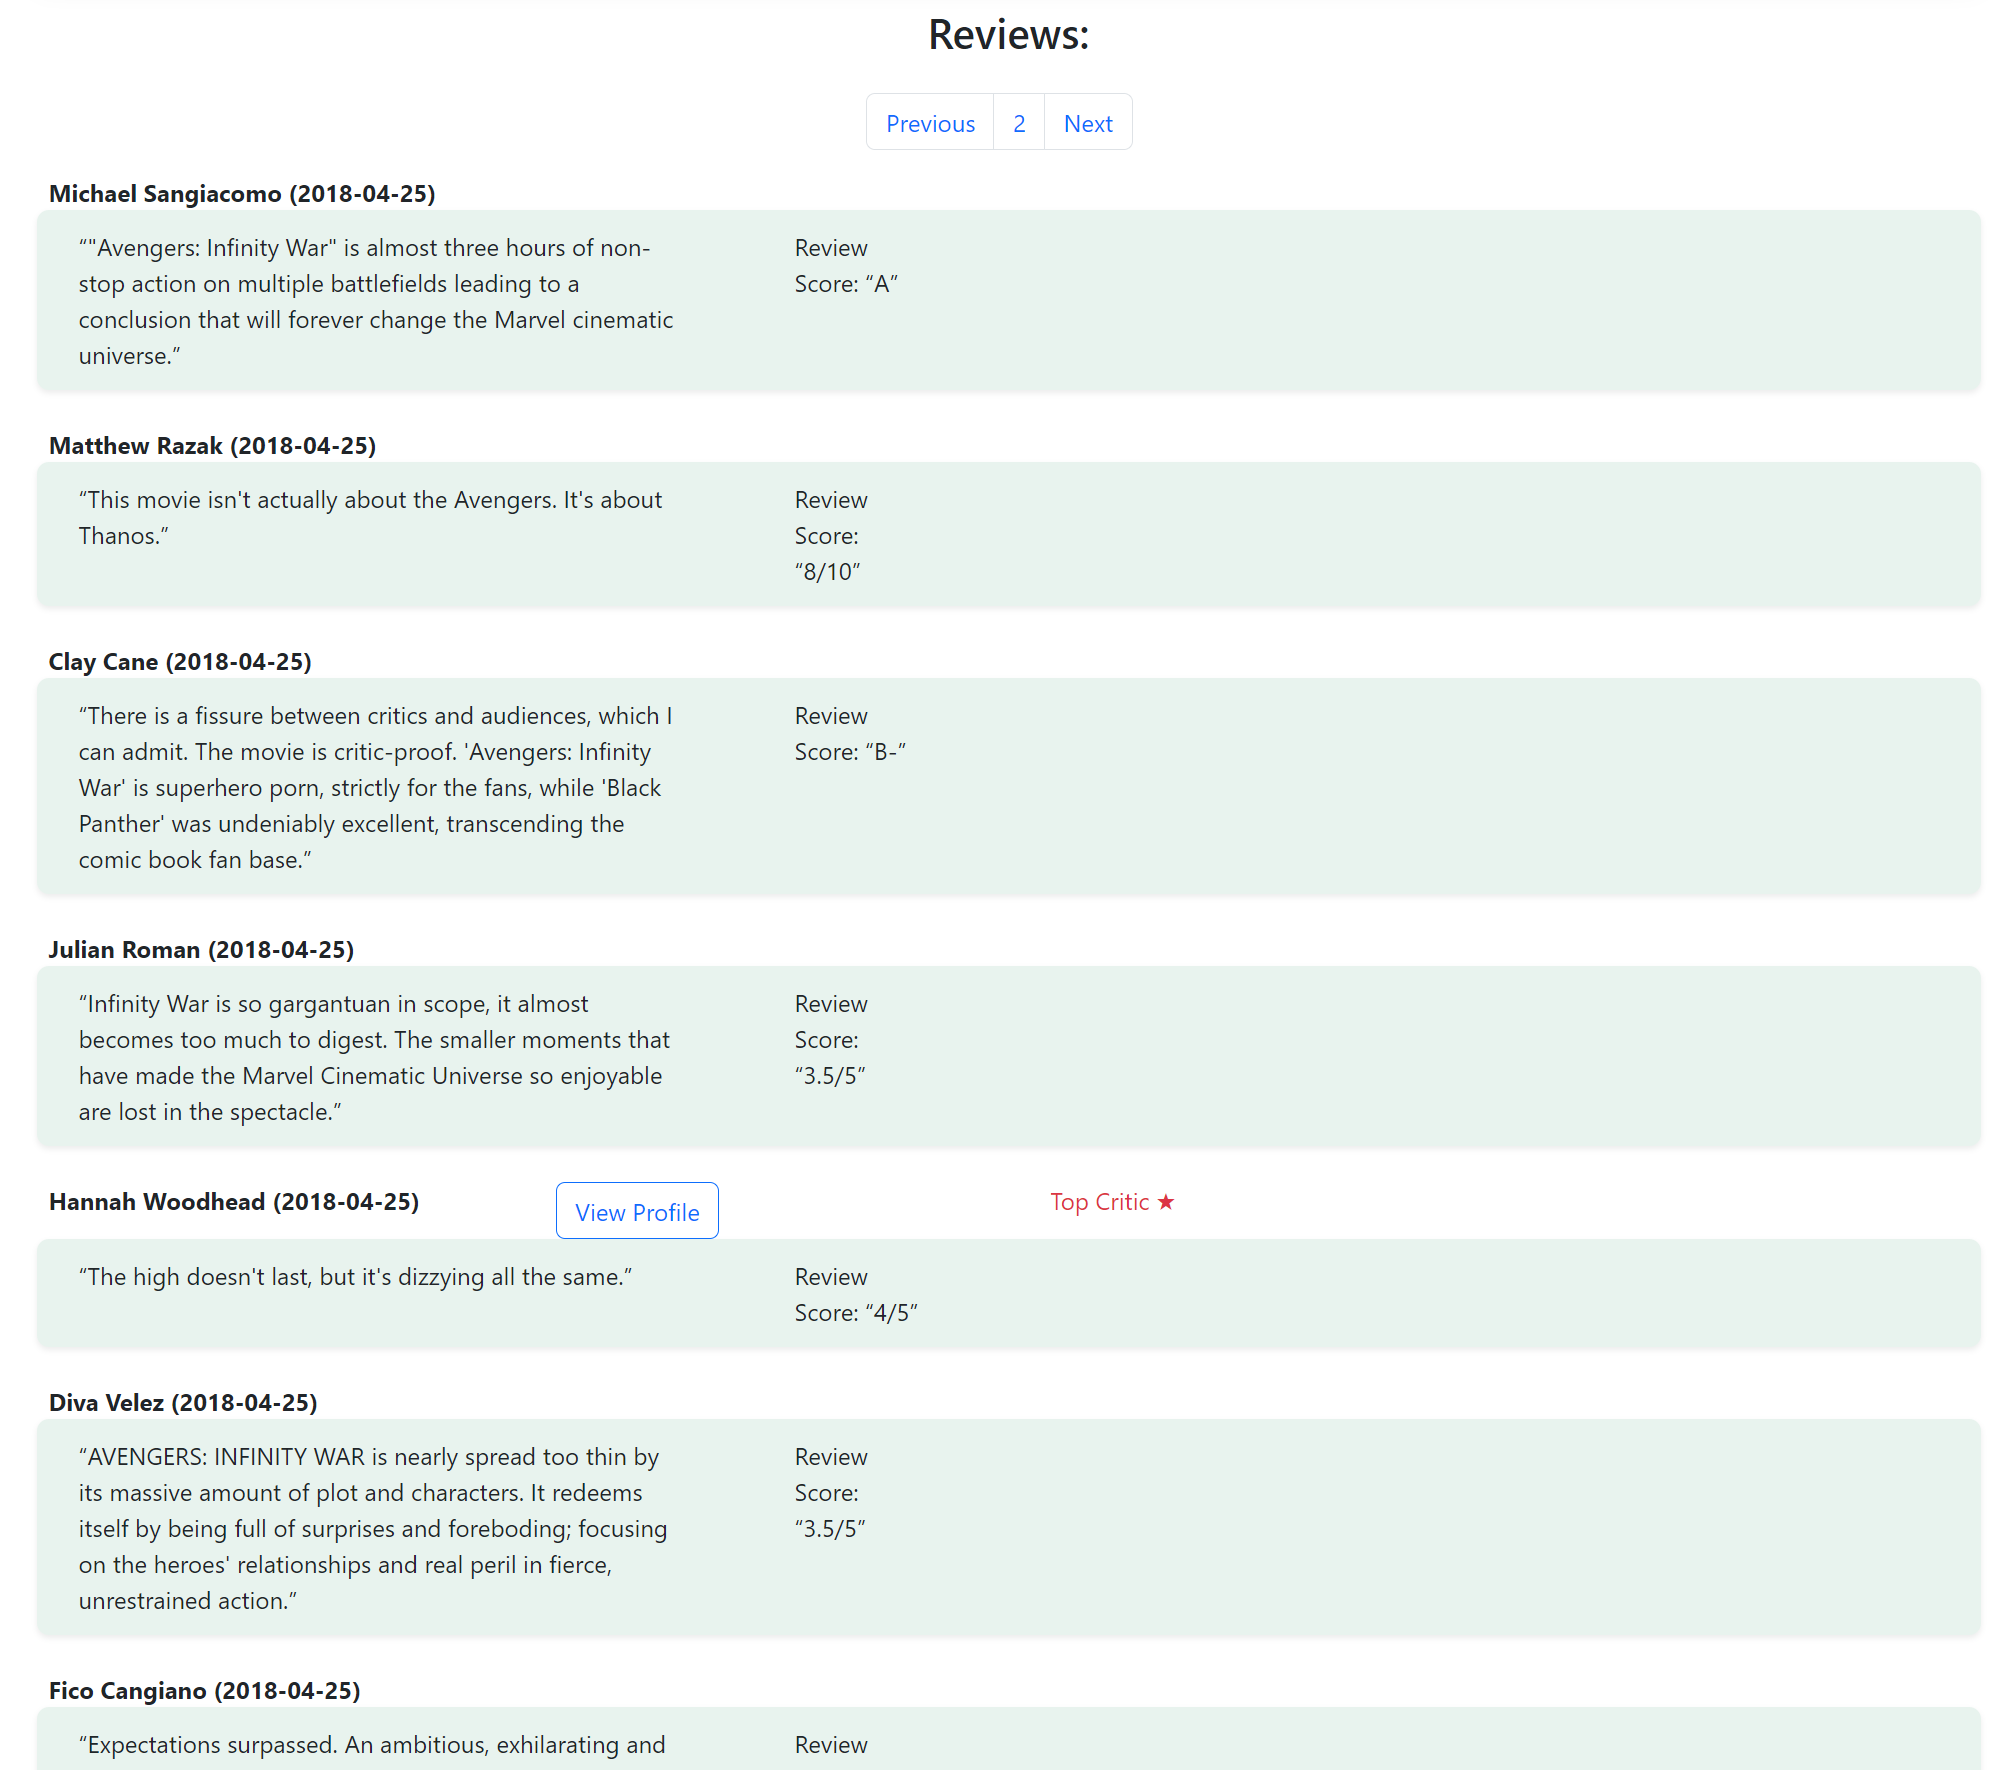
\includegraphics[scale=0.45]{../../../images/user_manual/reviews_under_movie.png} 

\end{center}
\vspace{5pt}
A selected movie allows also to read a paginated list of all its reviews

If a user isn't logged-in, the button under the movie says 'Login to Review this movie' and brings to the login page. Otherwise it becomes 'Review' and clicking on it allows the creation or editing of the review for that movie.

\begin{center}
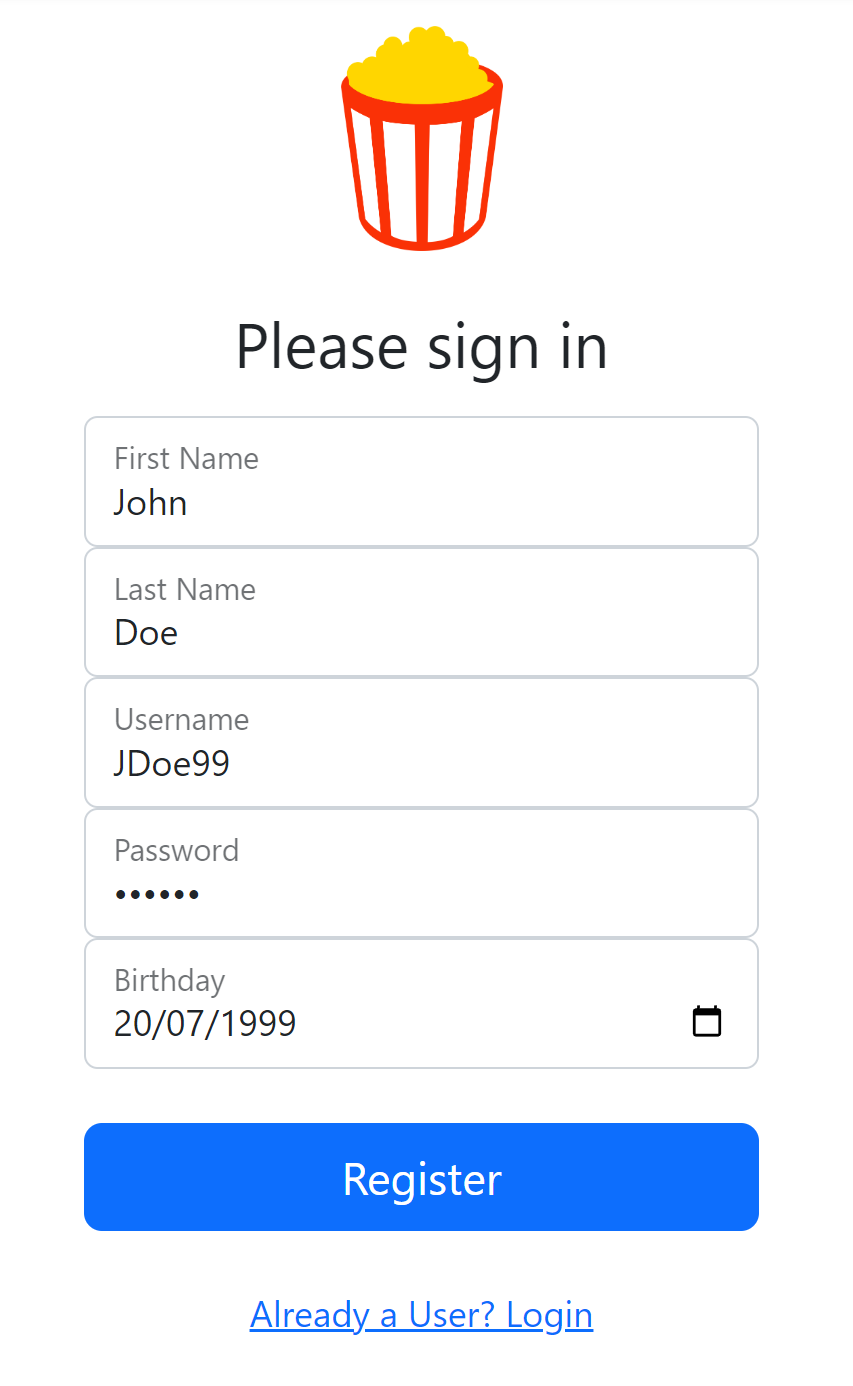
\includegraphics[scale=0.45]{../../../images/user_manual/user_registration.png} 
\end{center}
\vspace{5pt}

User registration requires some basic information about the new user
\begin{center}
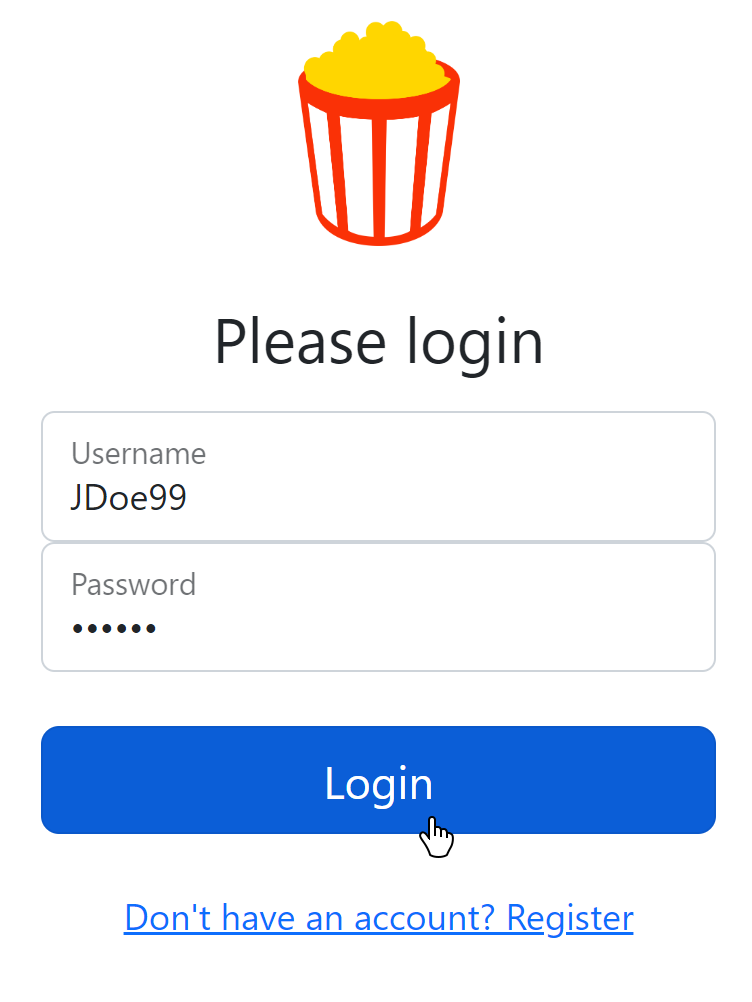
\includegraphics[scale=0.45]{../../../images/user_manual/login.png} 
\end{center}
\vspace{5pt}

If a user has already registered to the application, he/she can login with its credentials
\begin{center}
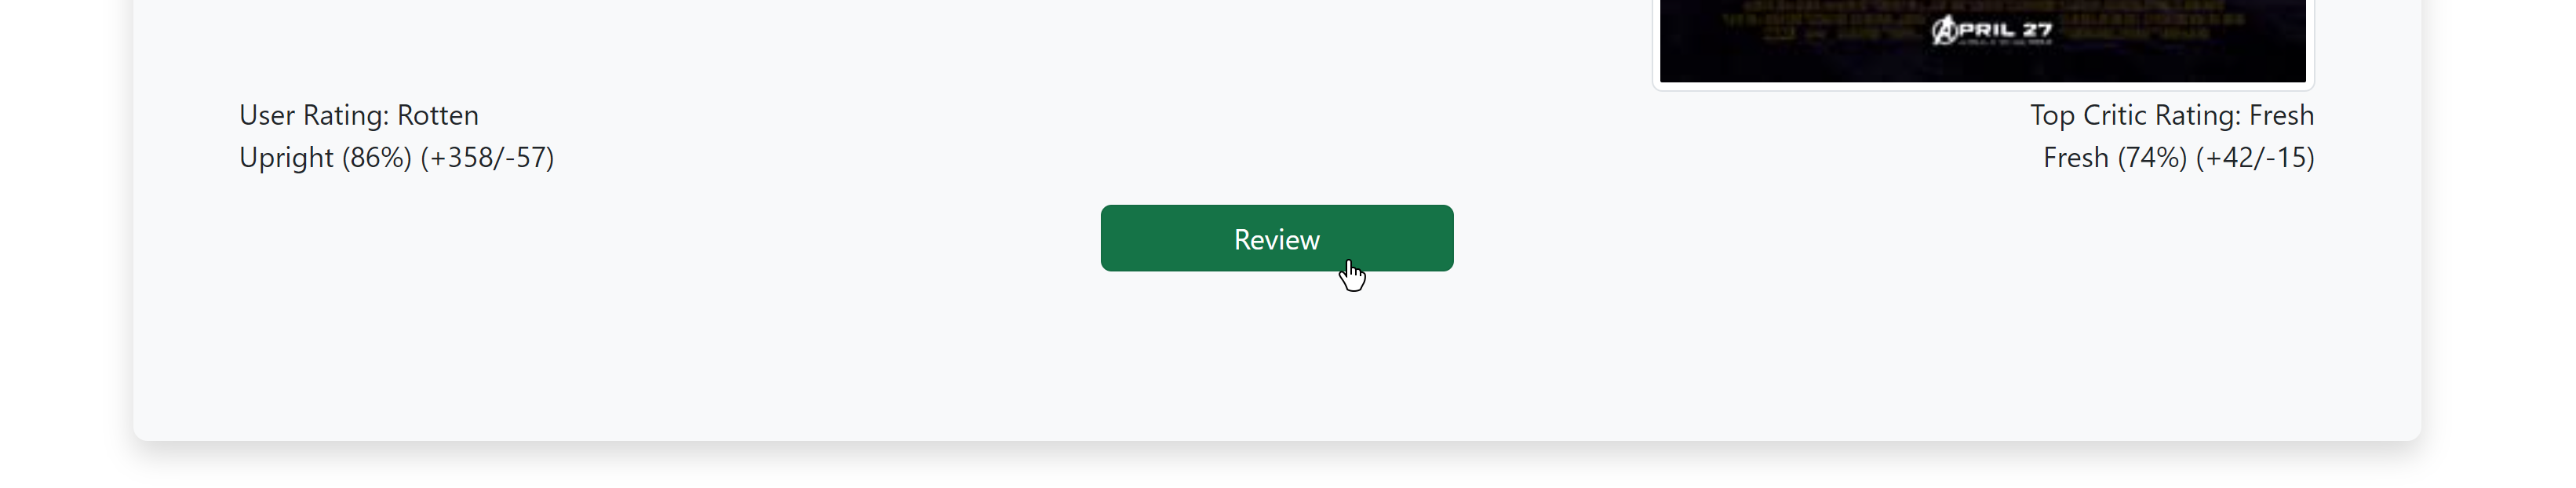
\includegraphics[scale=0.45]{../../../images/user_manual/review_button.png}
\end{center}
\vspace{5pt}

 
After logging-in, a user can leave a review under a movie

\begin{center}
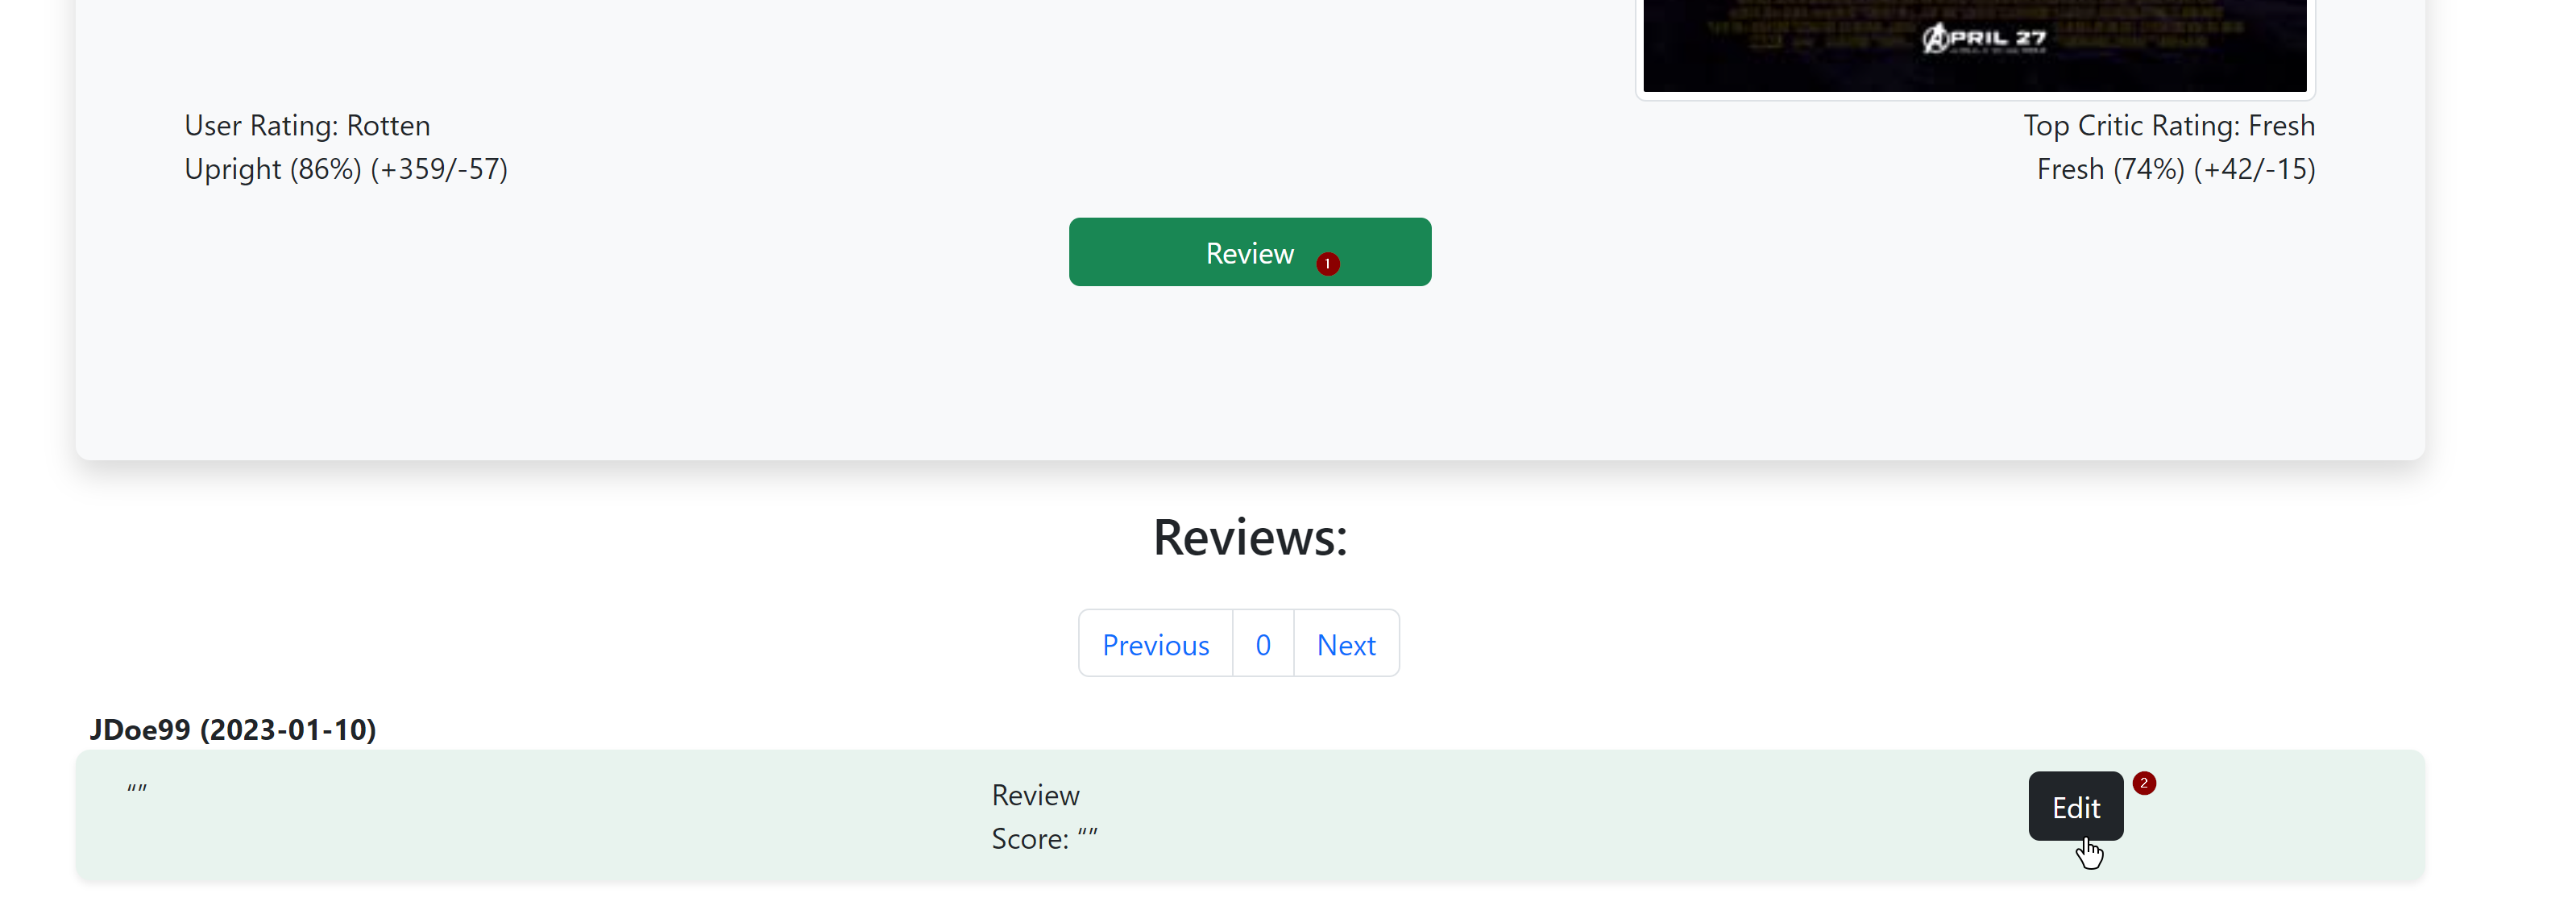
\includegraphics[scale=0.45]{../../../images/user_manual/new_review.png} 

\end{center}
\vspace{5pt}

If a user has never reviewed a movie, a new one is created and can be immediately modified

\begin{center}
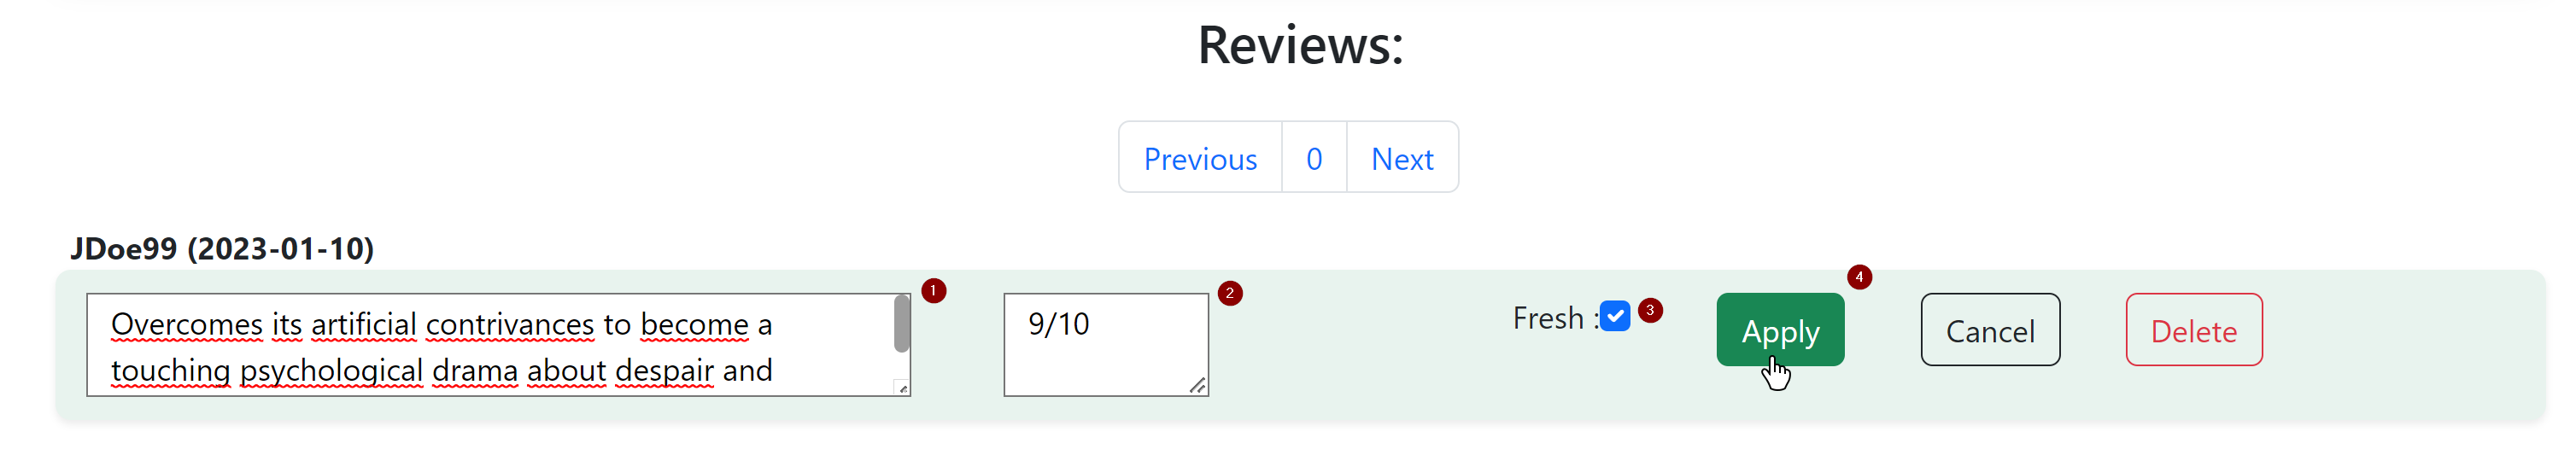
\includegraphics[scale=0.45]{../../../images/user_manual/write_review.png}
\end{center}
\vspace{5pt}
 

Writing a review, a user can write its content, leave a summarizing score and determine if it's a \textit{Fresh} (positive) or \textit{Rotten} (negative) review. Here the user can also choose to delete its review

\begin{center}

\includegraphics[scale=0.45]{../../../images/user_manual/view_profile_of_top_critic.png} 
\end{center}
\vspace{5pt}

Top Critic reviews are highlighted by a little label with a star and a link that brings to its user page

\begin{center}
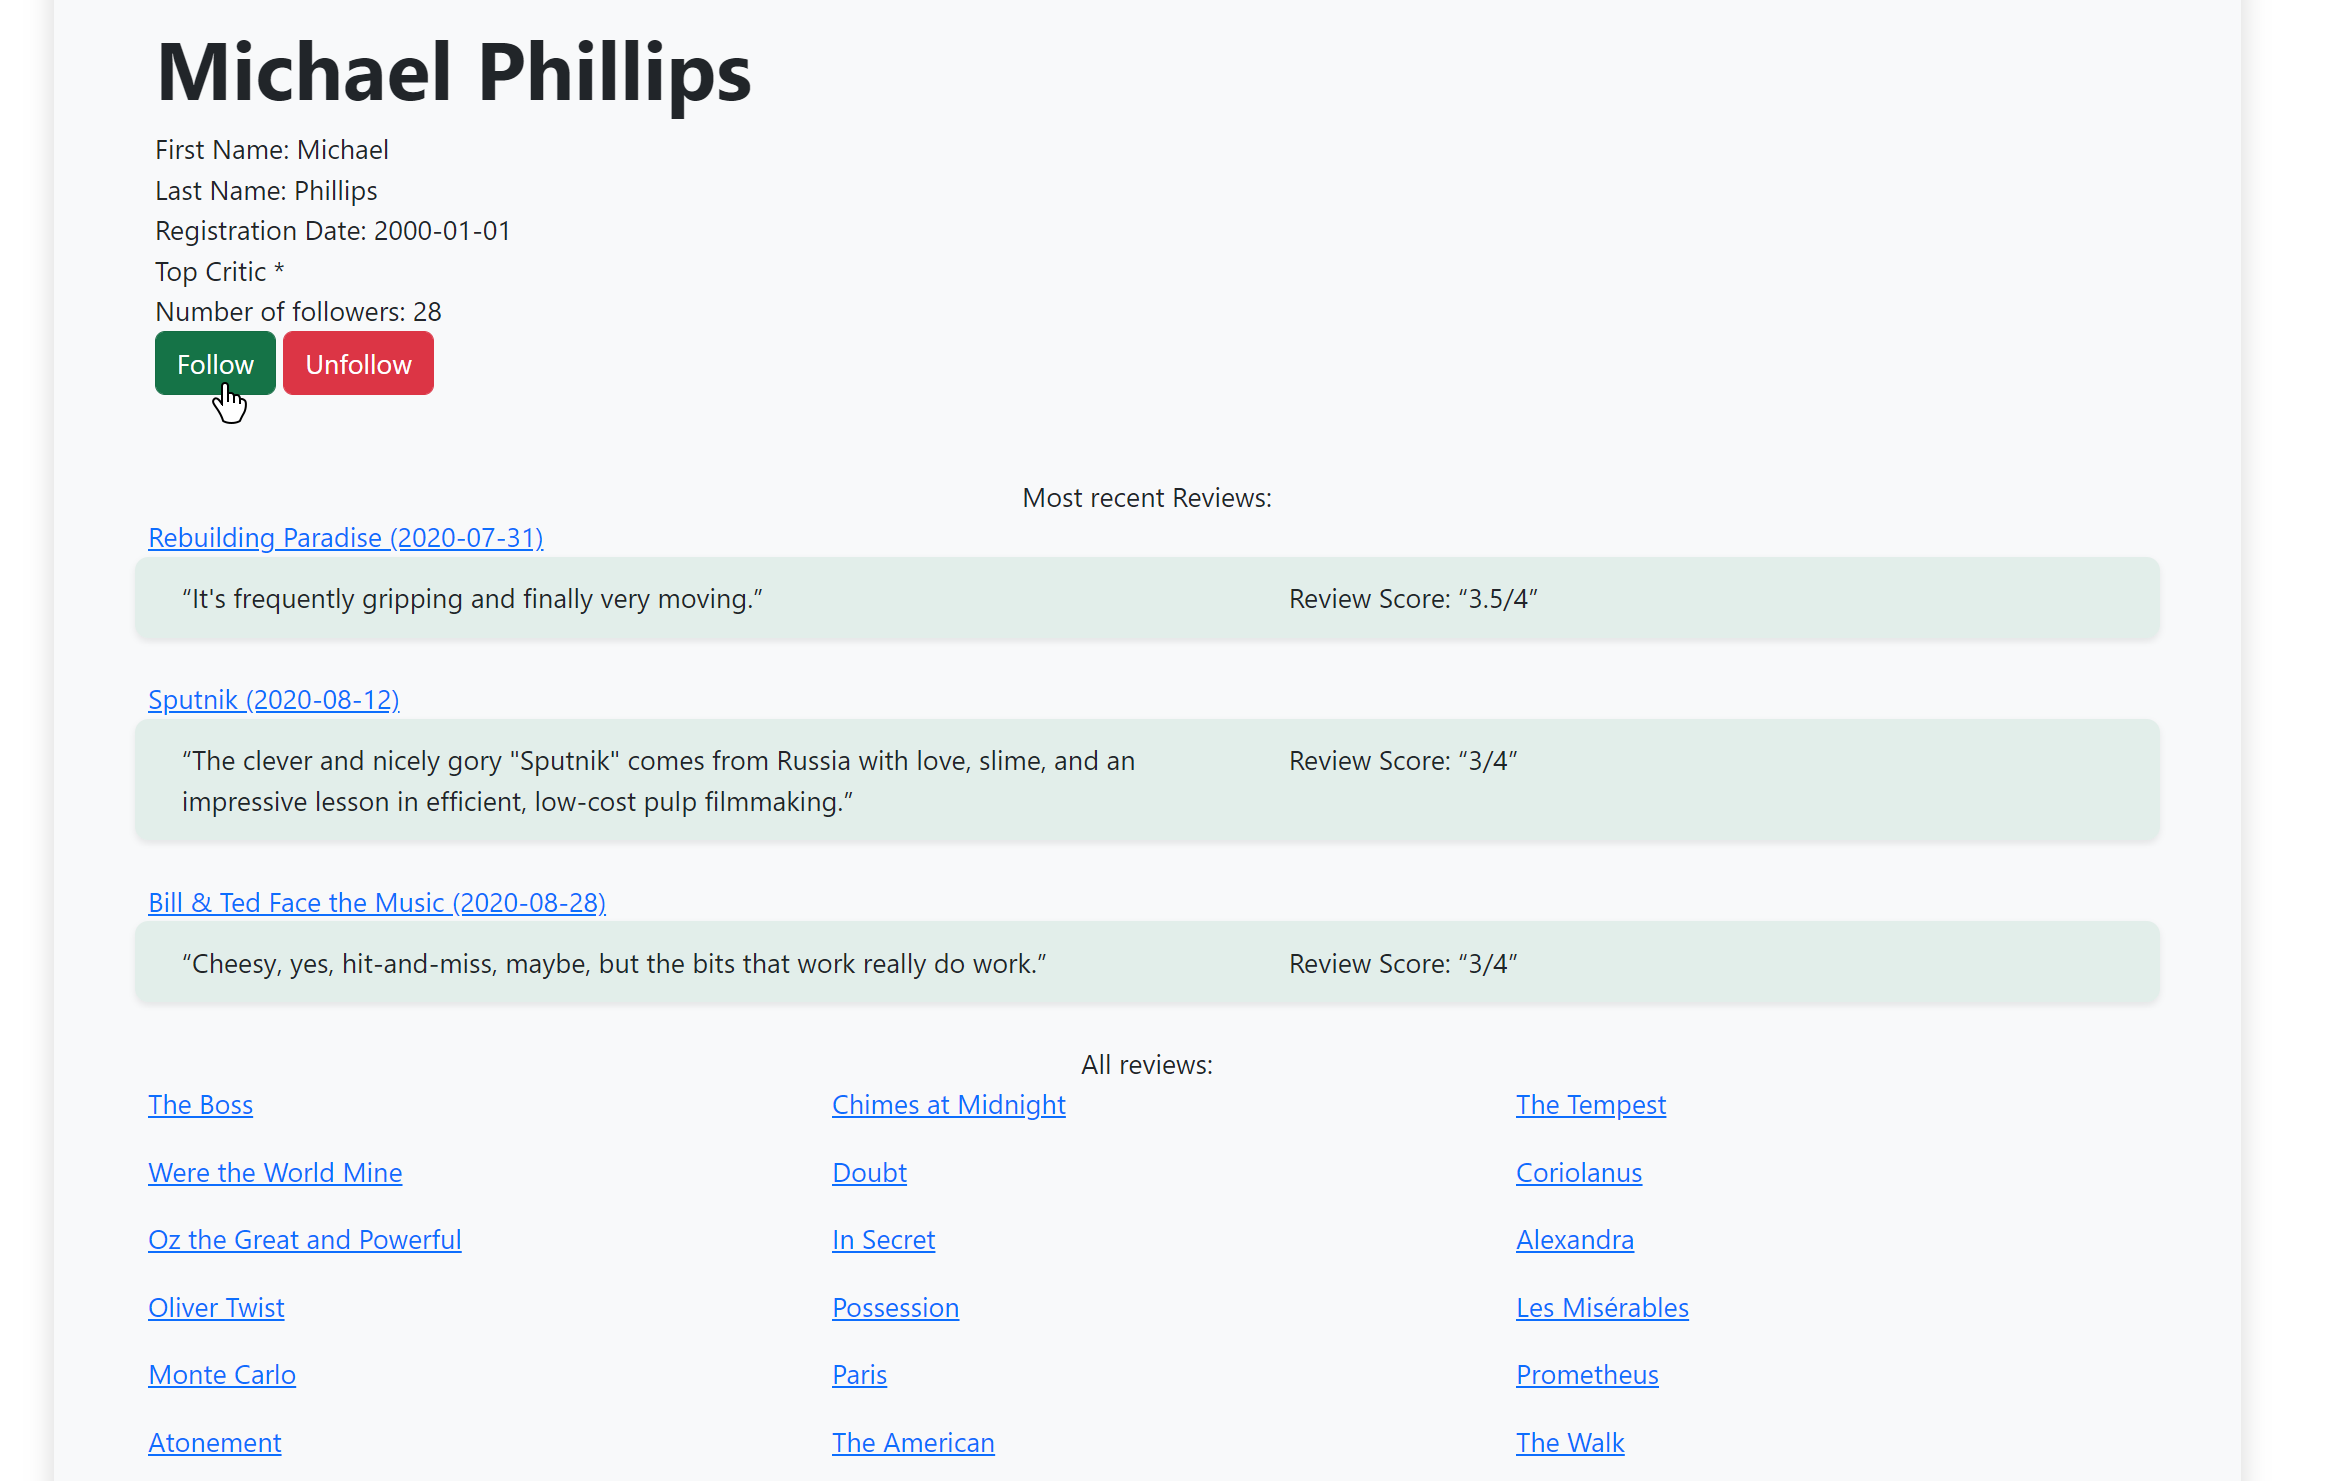
\includegraphics[scale=0.45]{../../../images/user_manual/follow_top_critic.png} 
\end{center}
\vspace{5pt}

Viewing the user page of a Top Critic, a user can choose to follow or, if its already a follower, unfollow that critic

\begin{center}
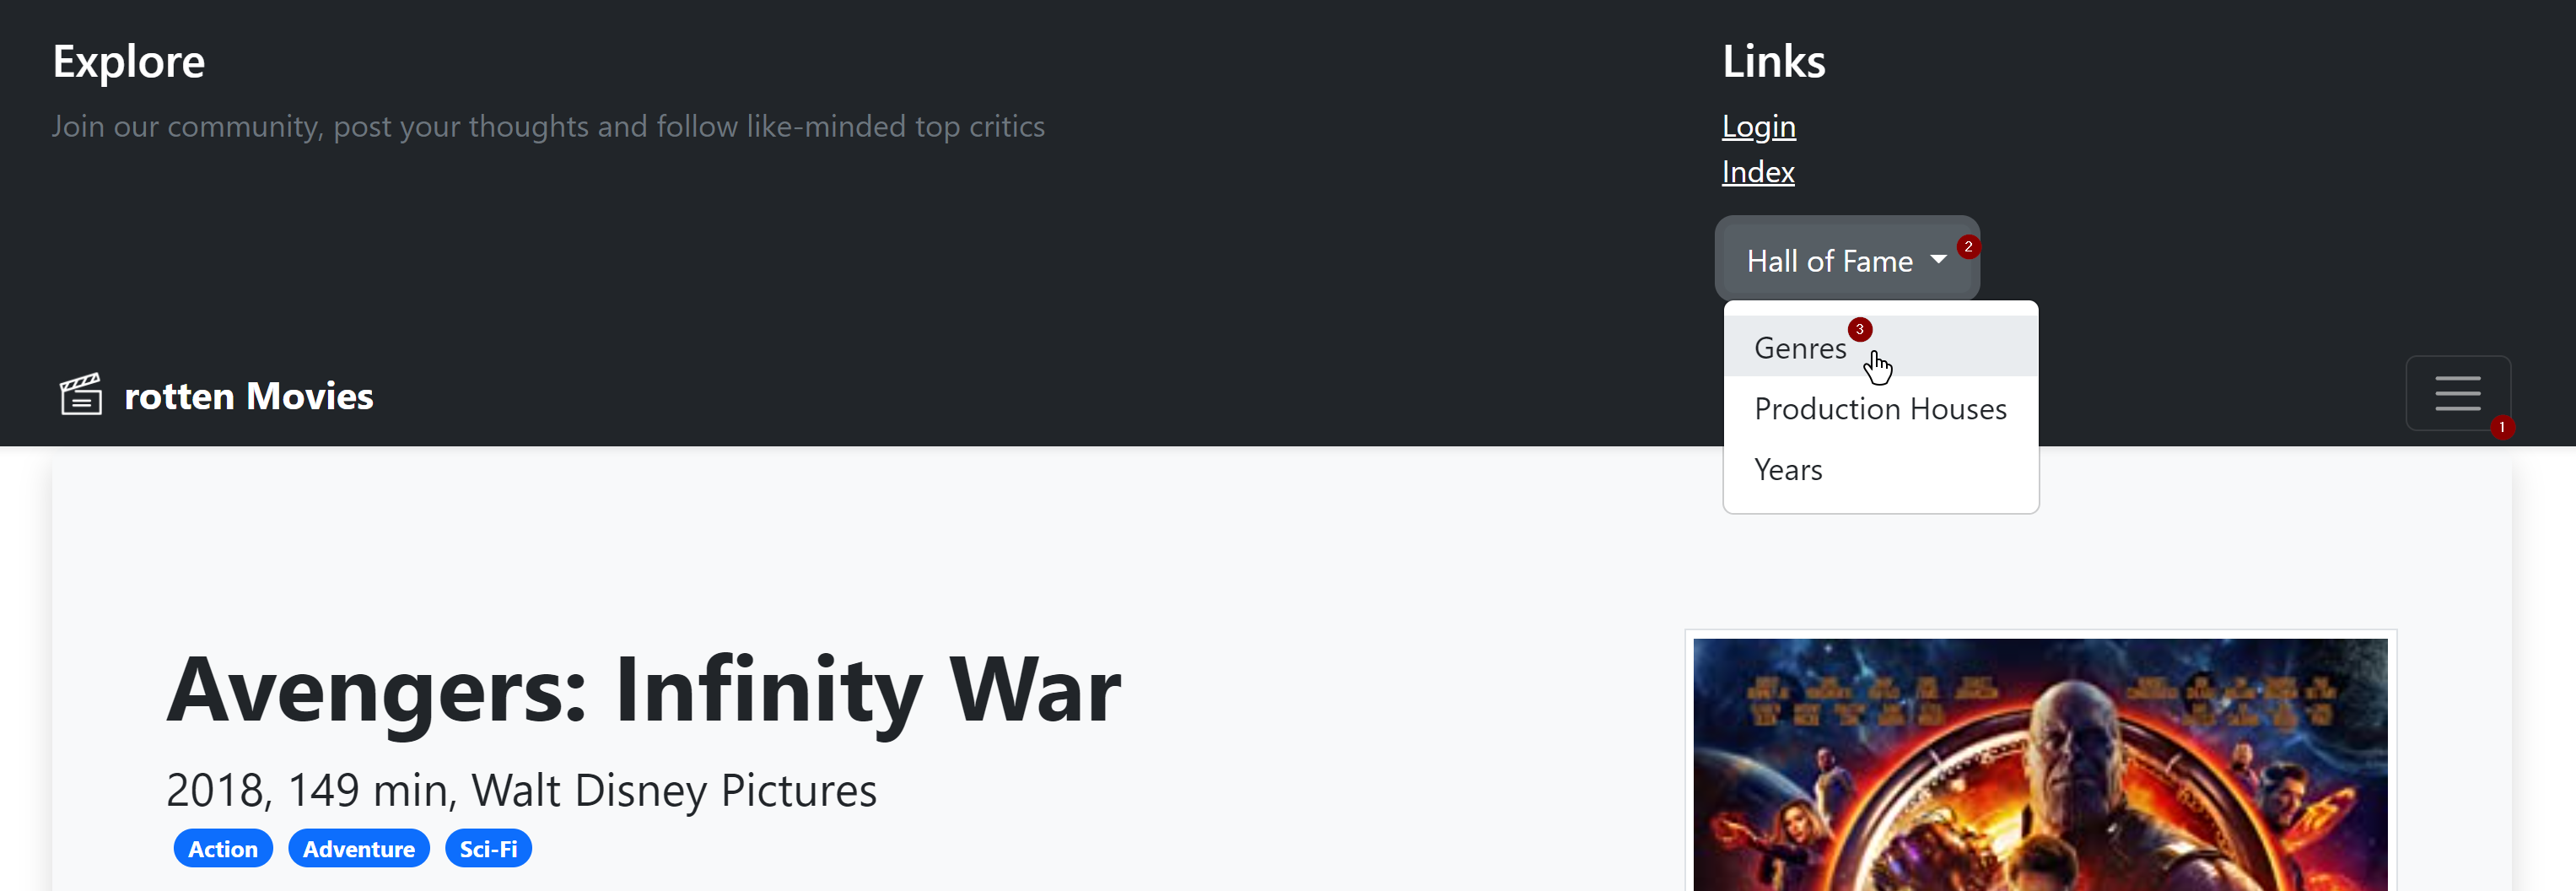
\includegraphics[scale=0.45]{../../../images/user_manual/unregistered_navbar.png} 
\end{center}
\vspace{5pt}

The navbar for a user that hasn't logged-in has some basic features

\begin{center}
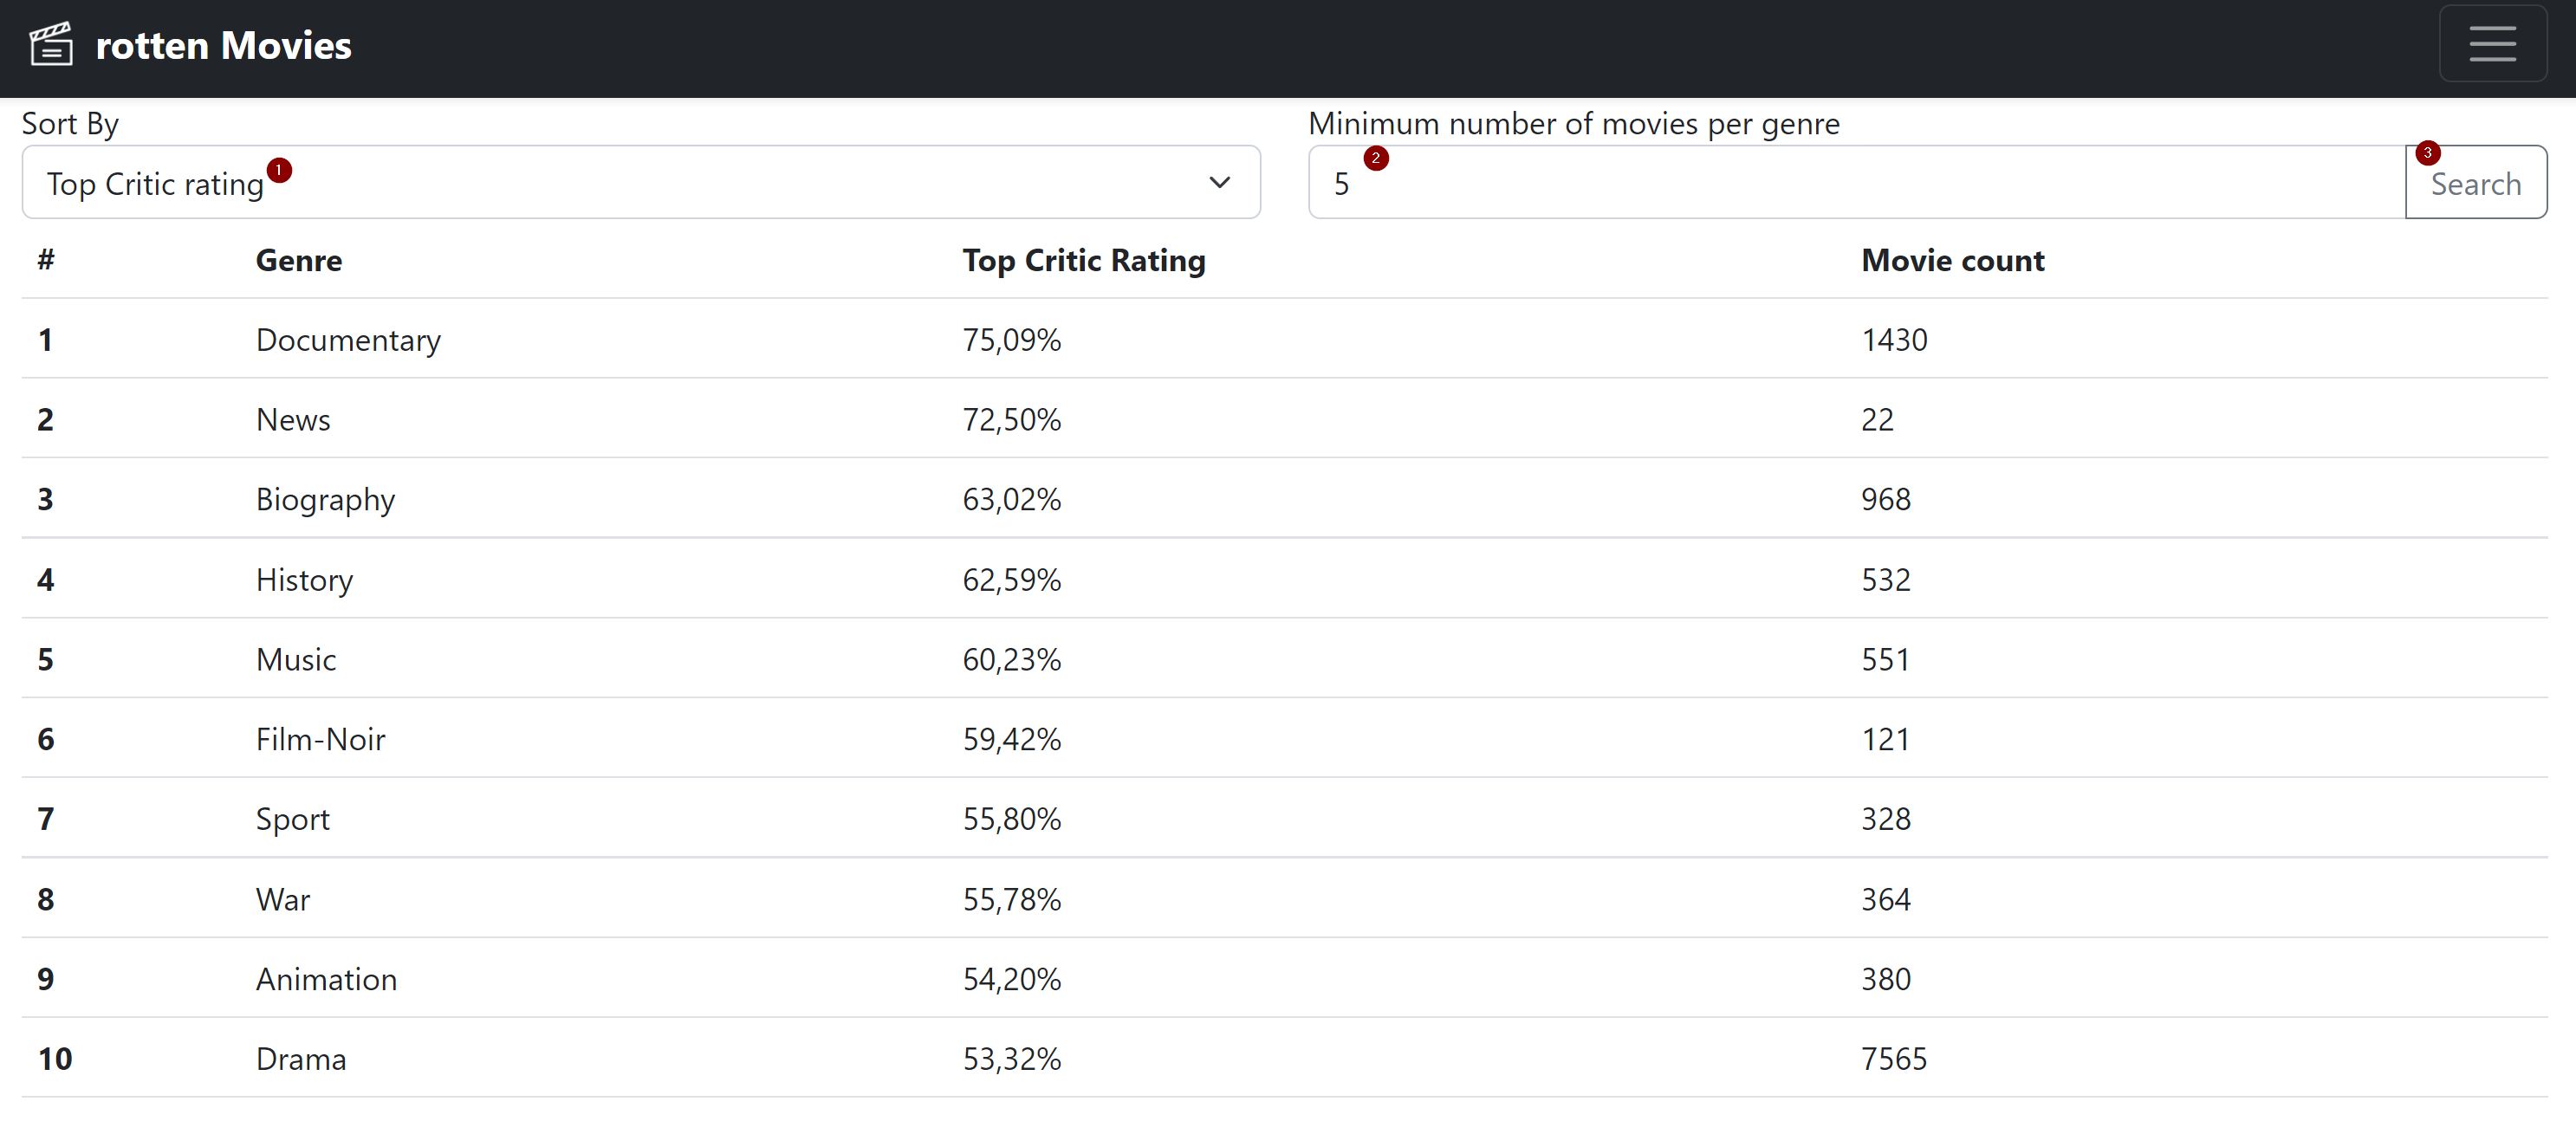
\includegraphics[scale=0.45]{../../../images/user_manual/best_genres.png} 
\end{center}
\vspace{5pt}

This page shows the best genres across all movies, sorted by top critic rating or user rating. It is also possible to specify the minimum number of movies that a genre must have to appear in the list

\begin{center}
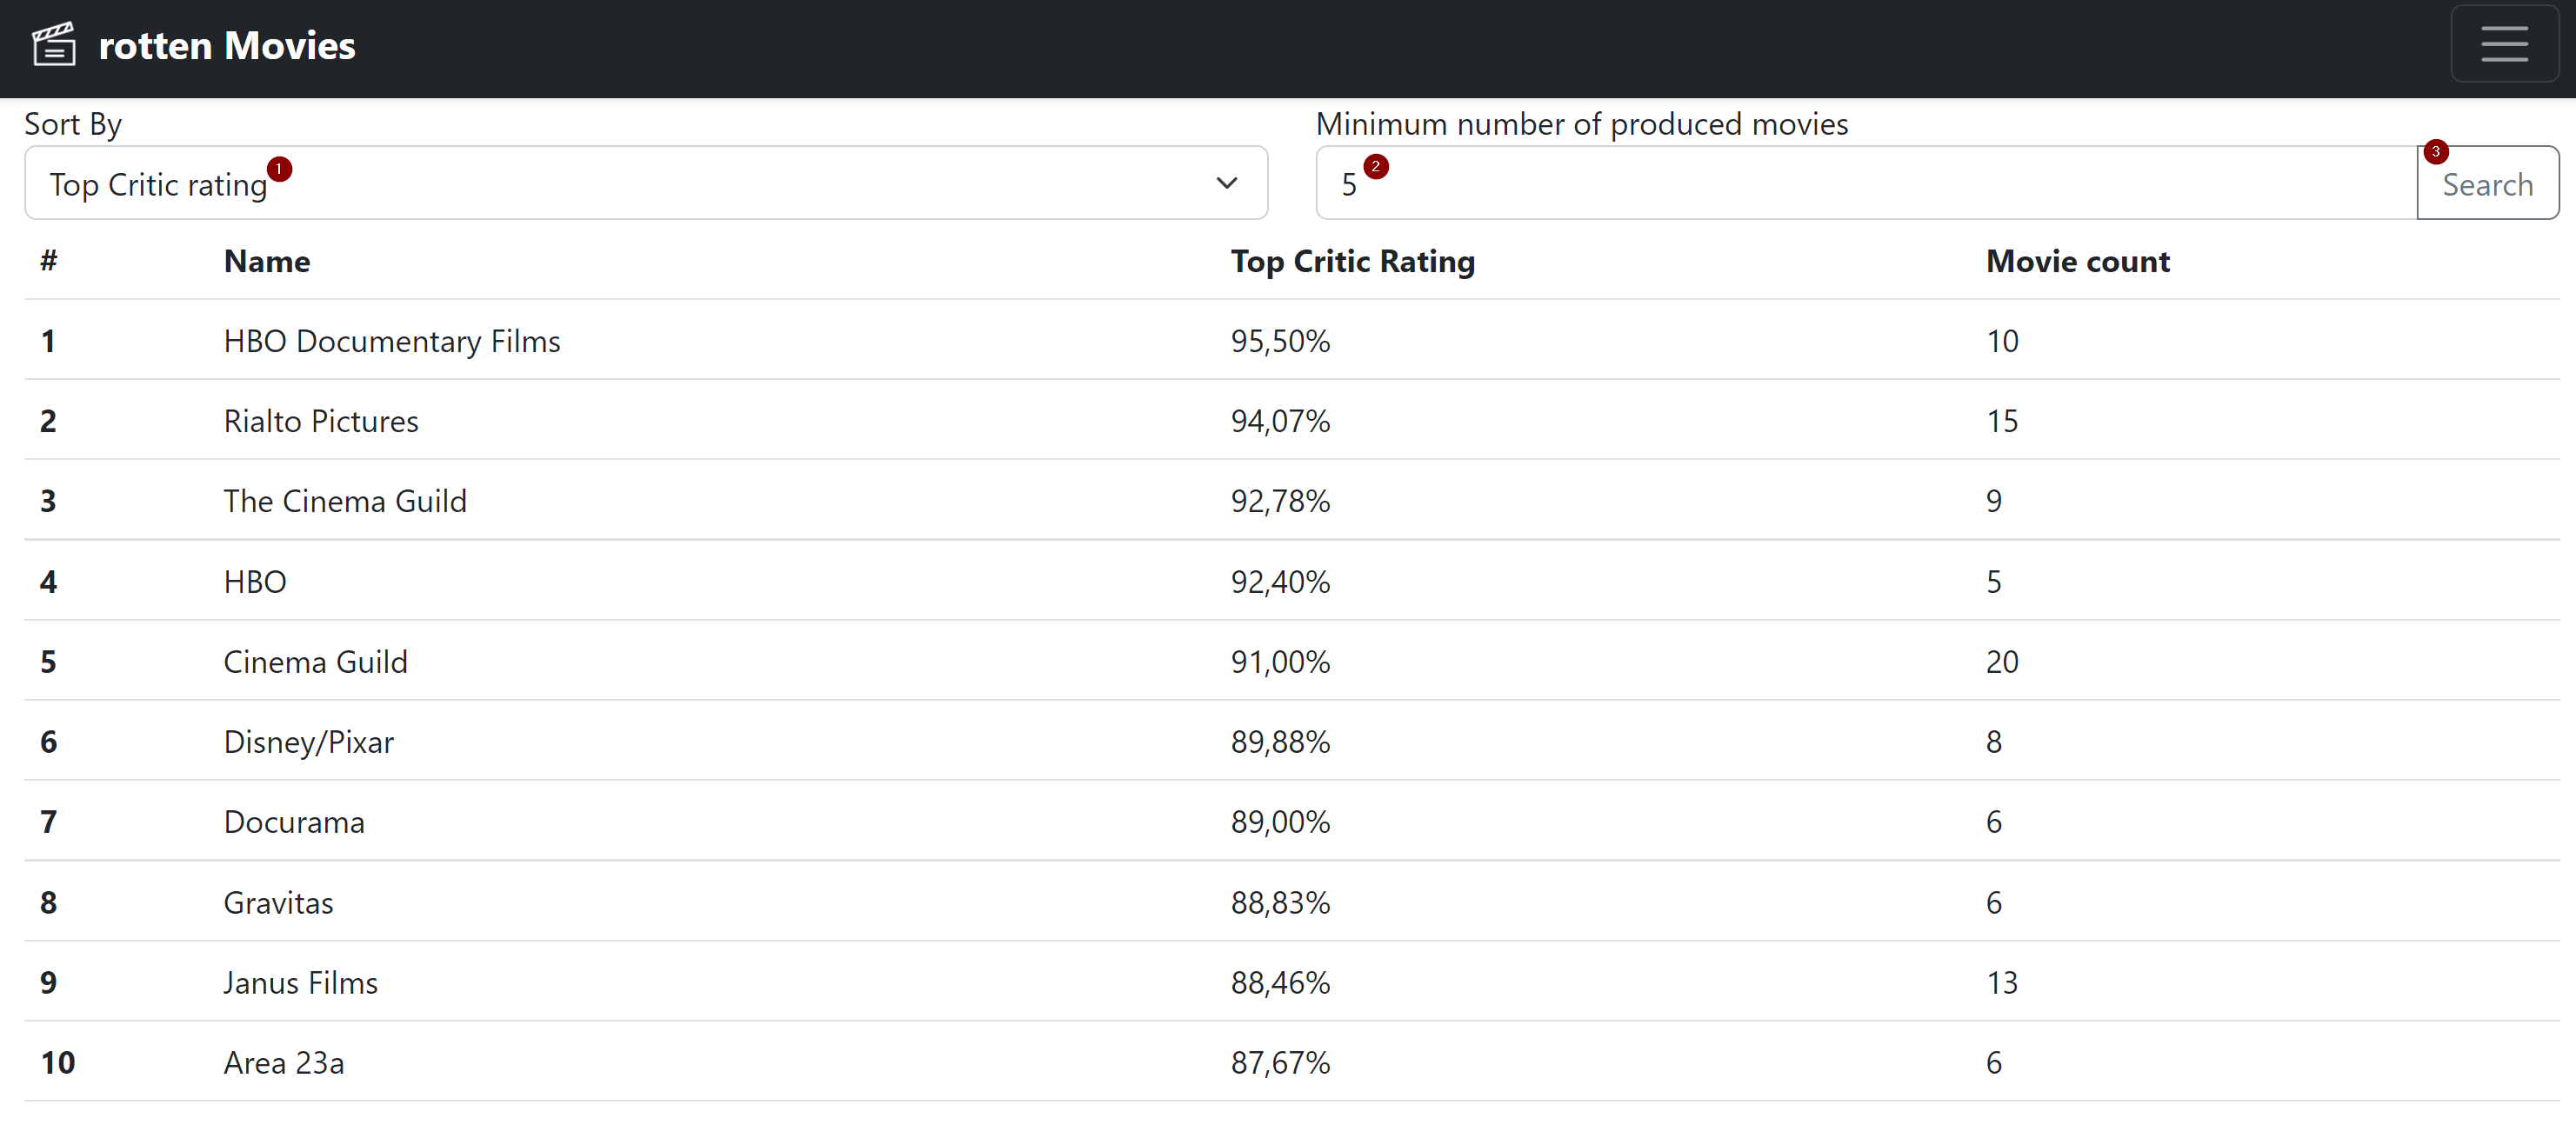
\includegraphics[scale=0.45]{../../../images/user_manual/best_production_houses.png}
\end{center}
\vspace{5pt}

This page shows the best production houses based on the reviews left by users on the platform. They can be sorted by top critic rating or user rating and the user can specify the minimum number of produced movies to appear on the list

\begin{center}
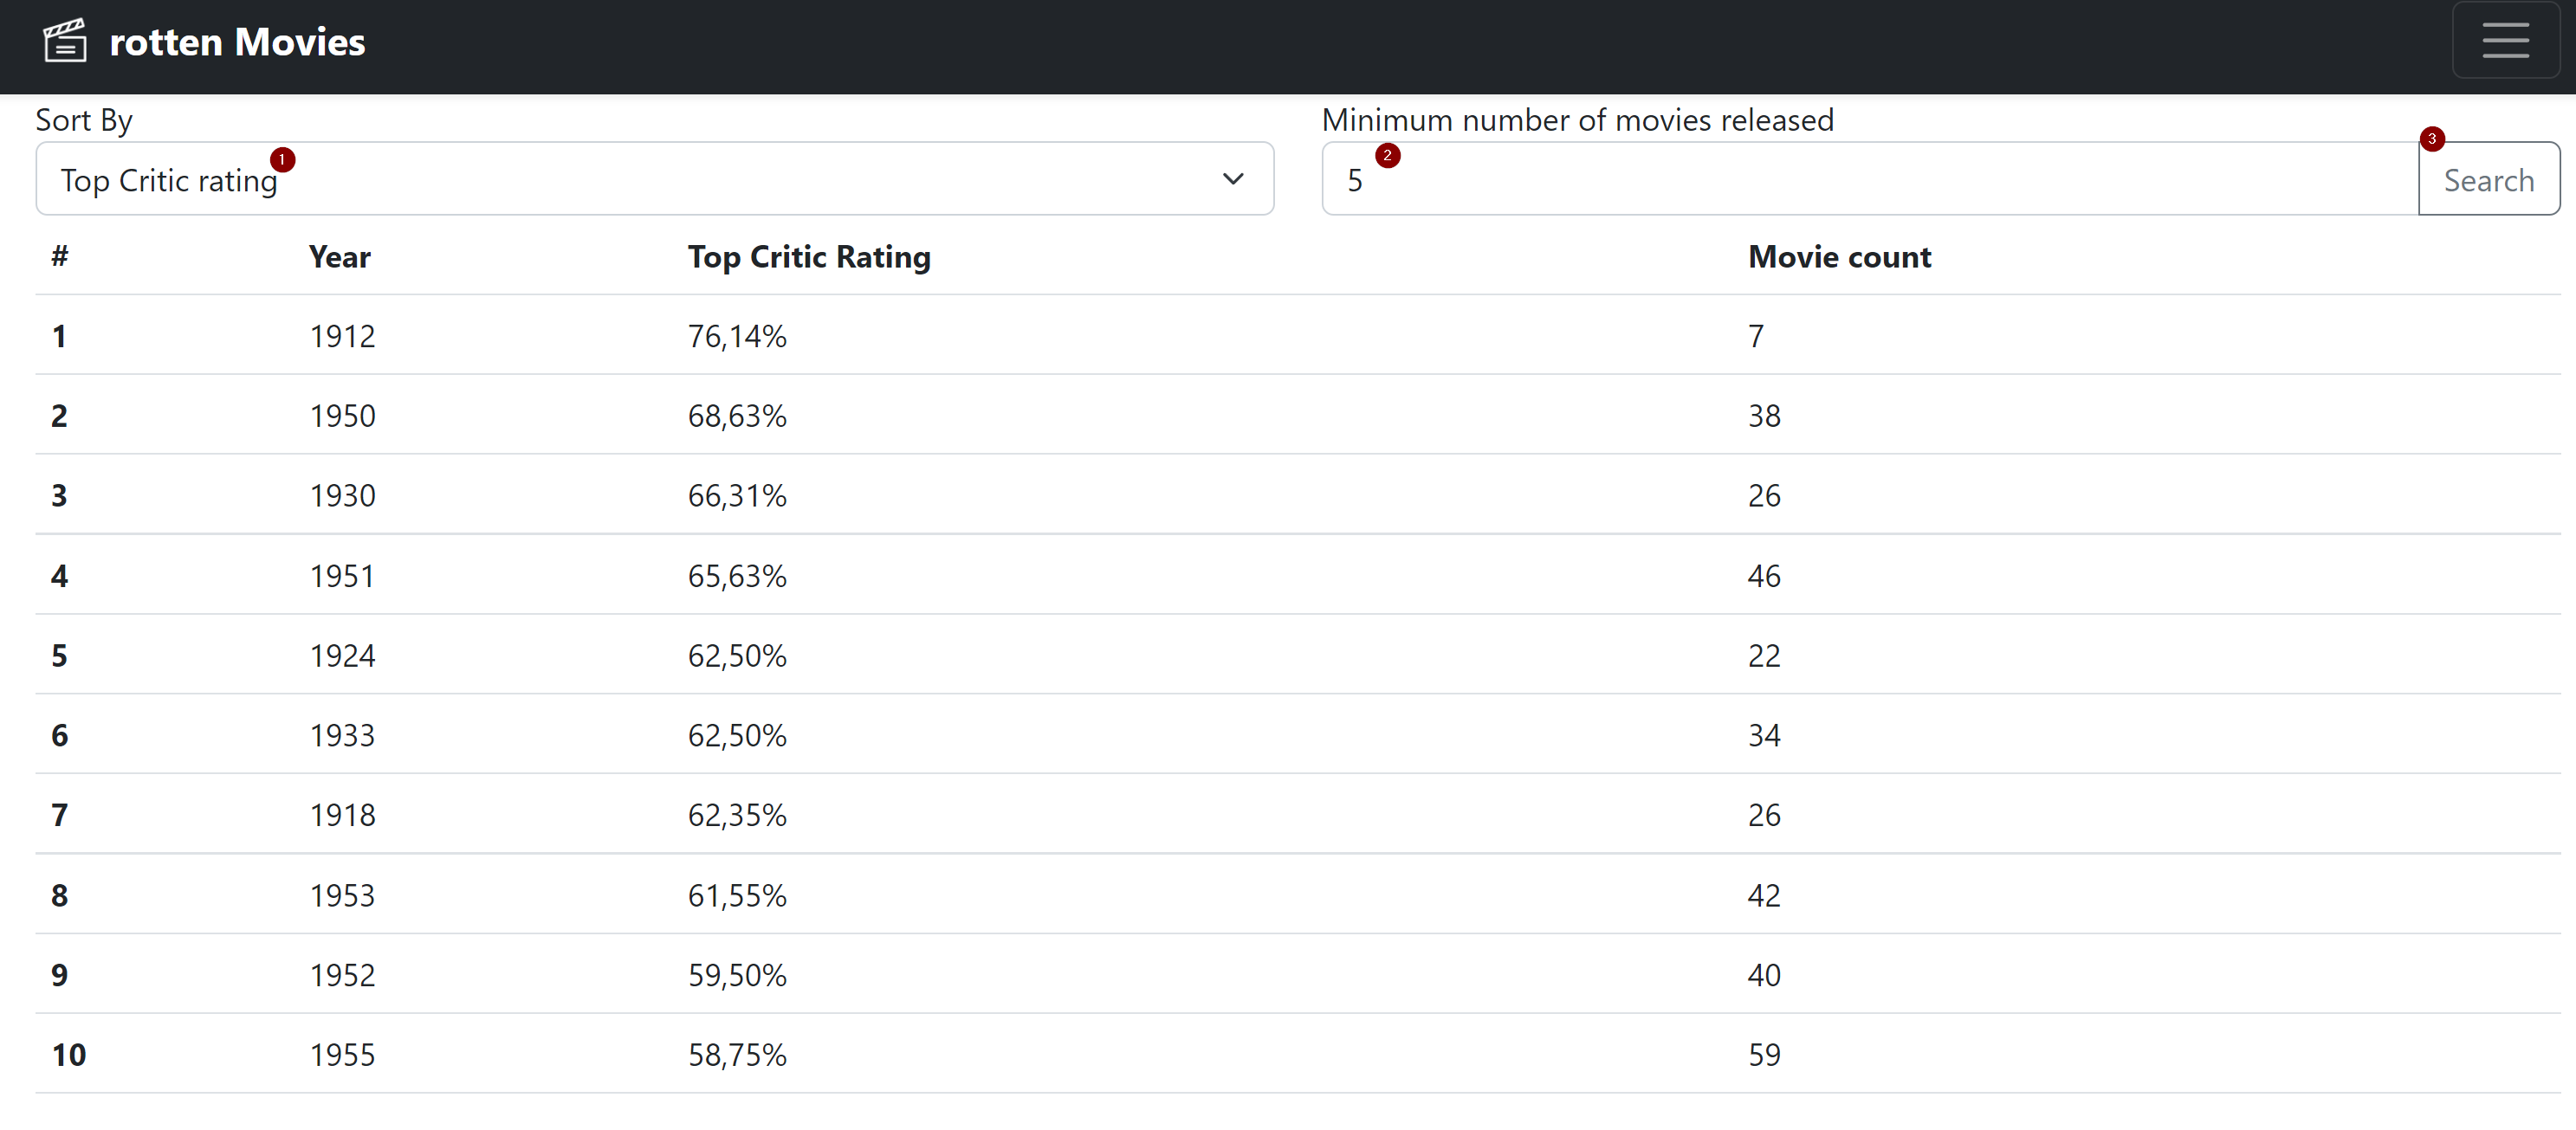
\includegraphics[scale=0.45]{../../../images/user_manual/best_years.png} 
\end{center}


This page shows the best years in terms of produced movies with positive reviews left by users on the platform. They can be sorted by top critic rating or user rating and the user can specify the minimum number of released movies in that year to appear on the list

\begin{center}
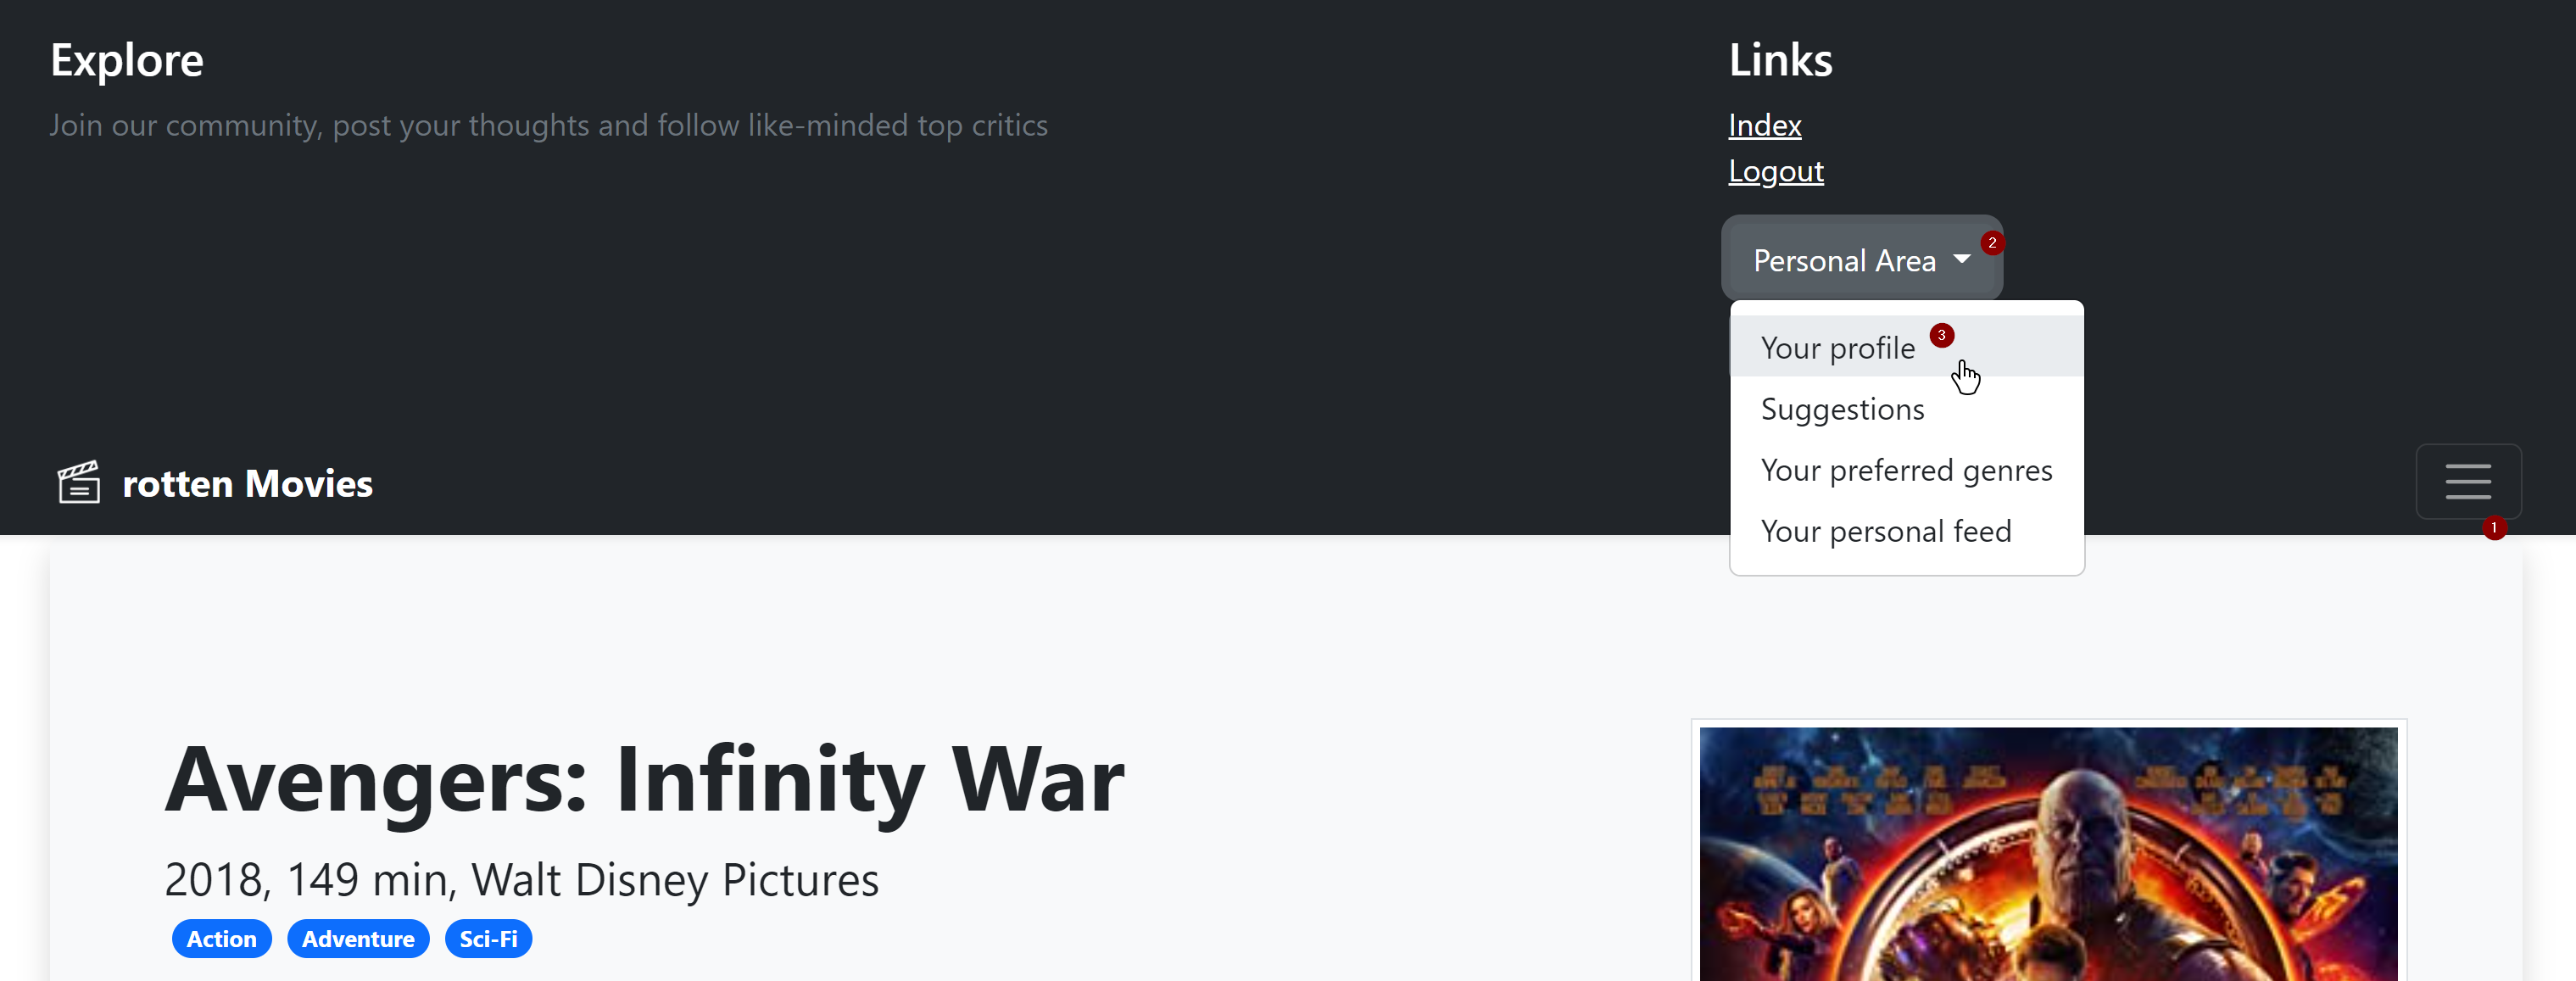
\includegraphics[scale=0.45]{../../../images/user_manual/authenticated_navbar.png} 
\end{center}
\vspace{5pt}

The navbar of an authenticated user shows some more personalized pages

\begin{center}
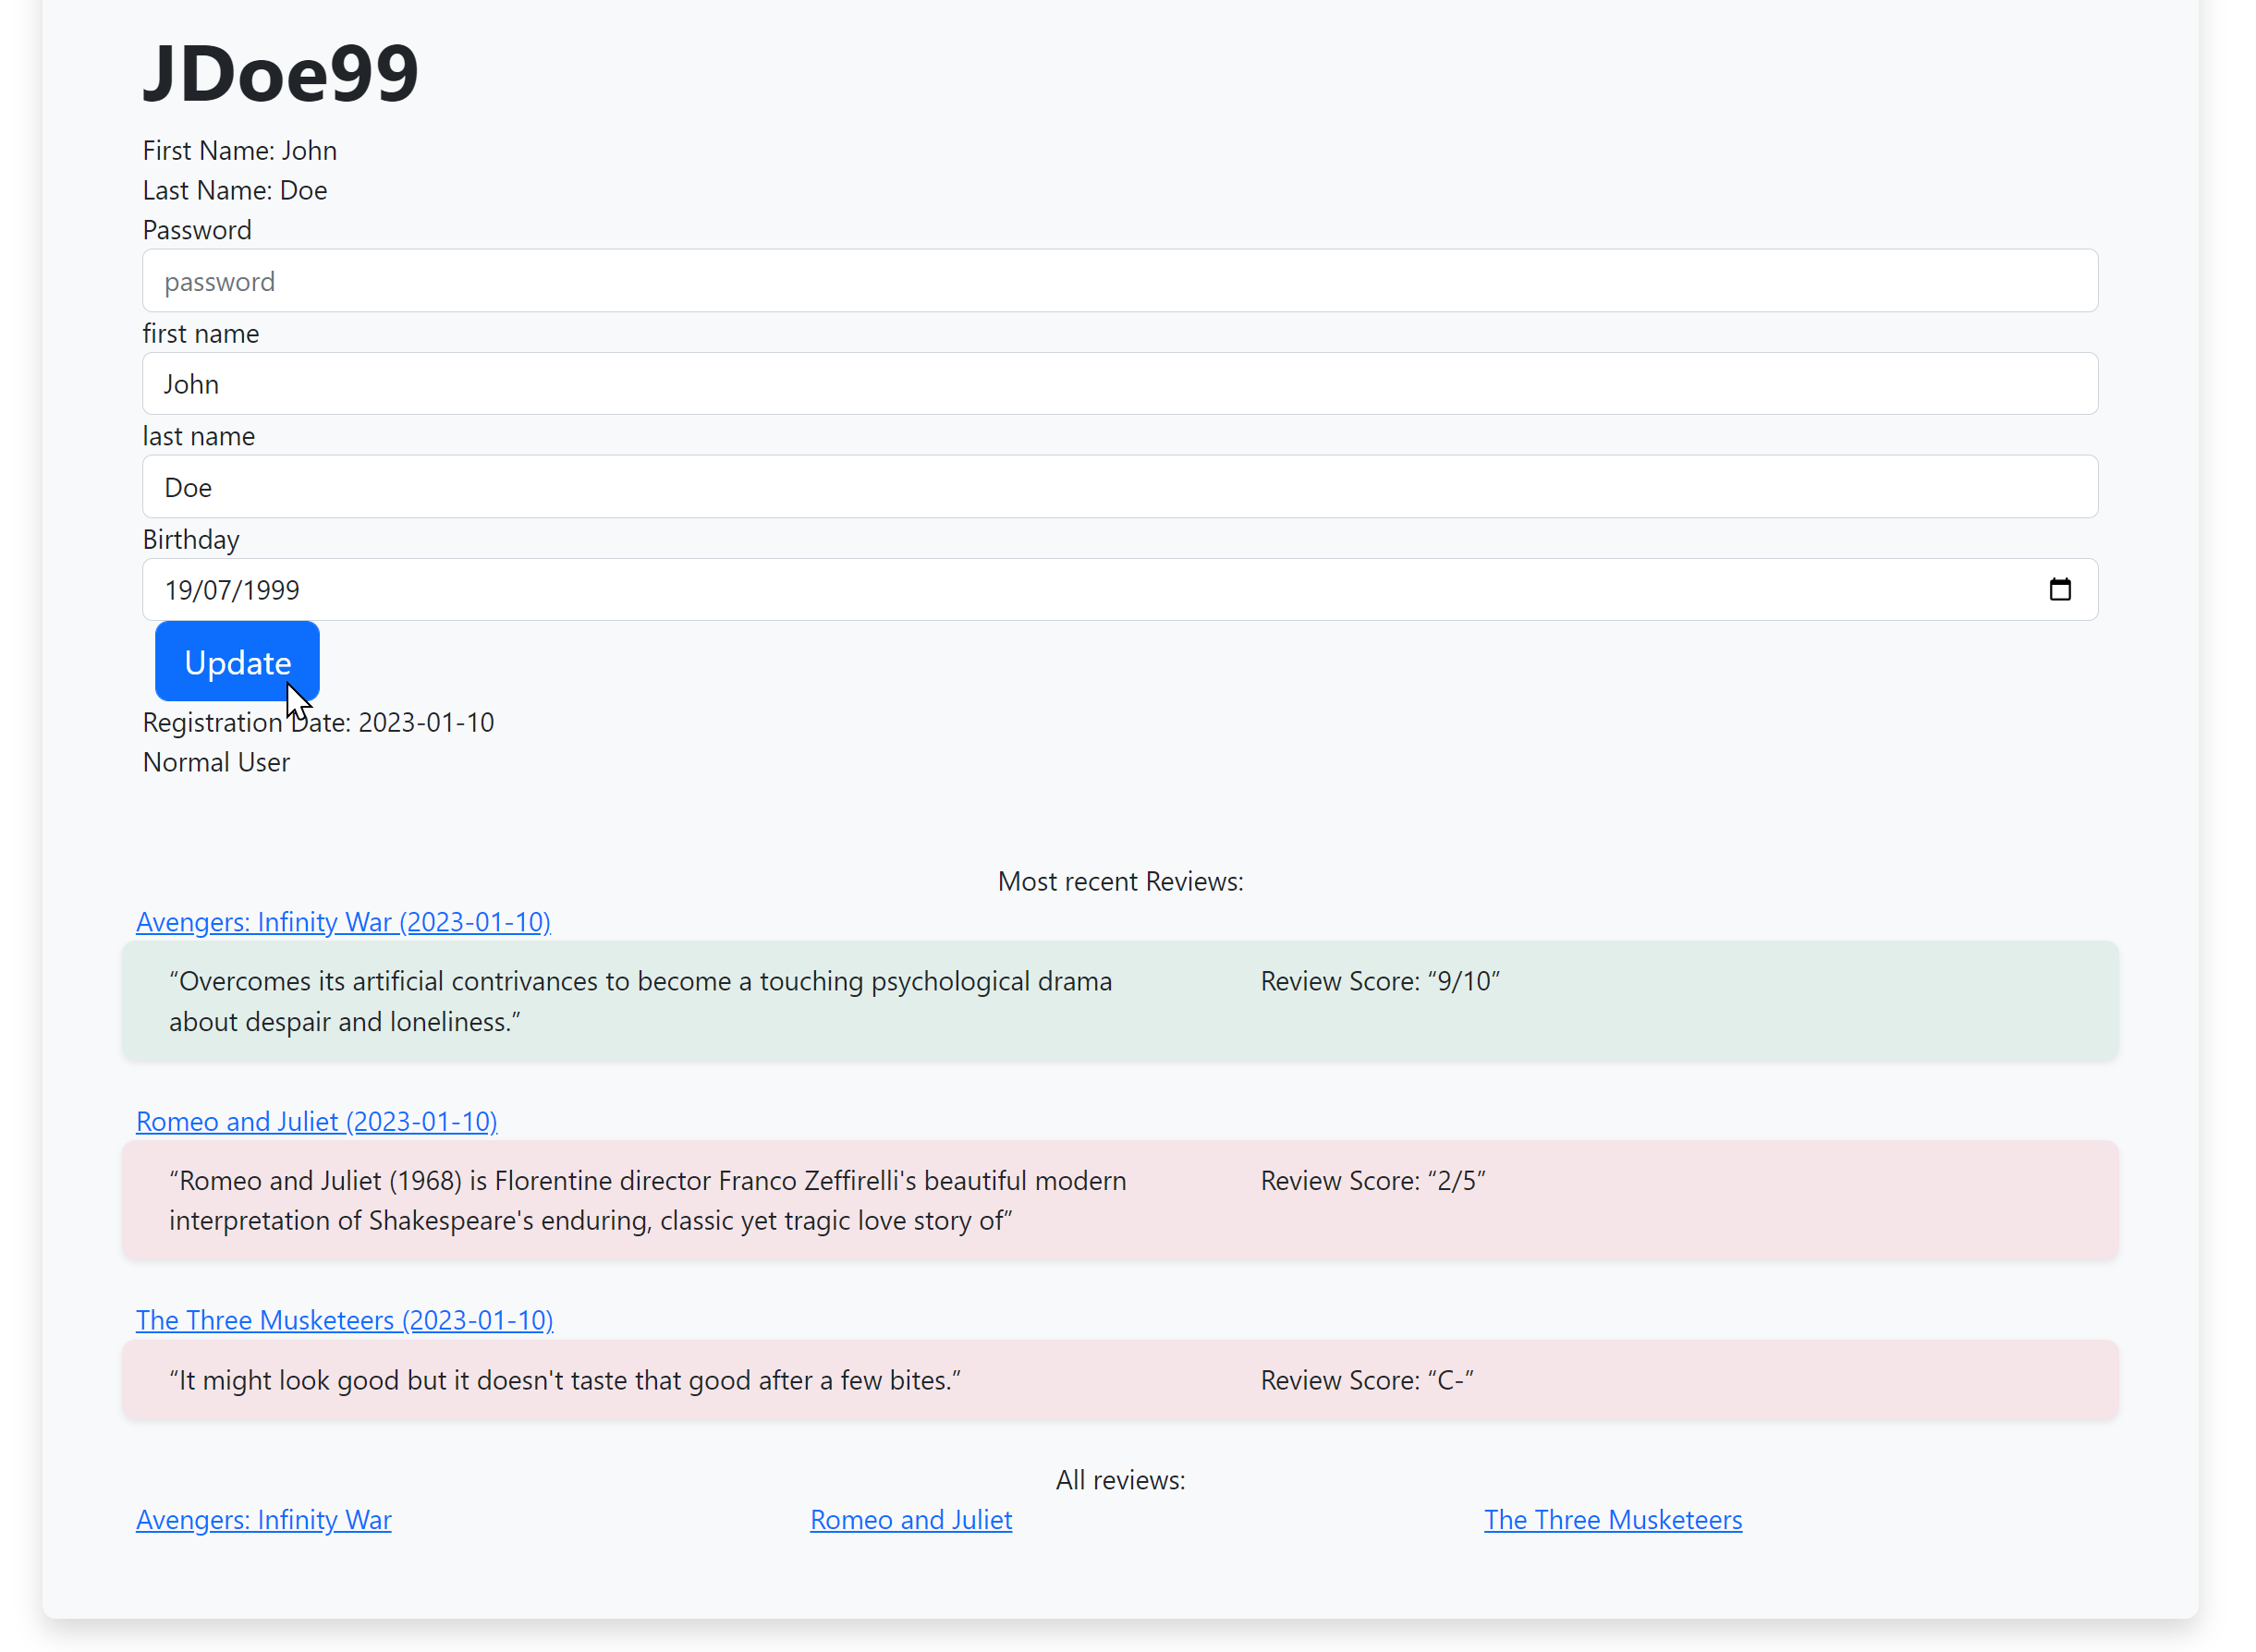
\includegraphics[scale=0.45]{../../../images/user_manual/personal_page.png}
\end{center}
 \vspace{5pt}

In the personal page, a user can change its credentials, see its three most recent reviews and the list of all its reviewed movies.

Leaving the password field blank won't change it.

\begin{center}
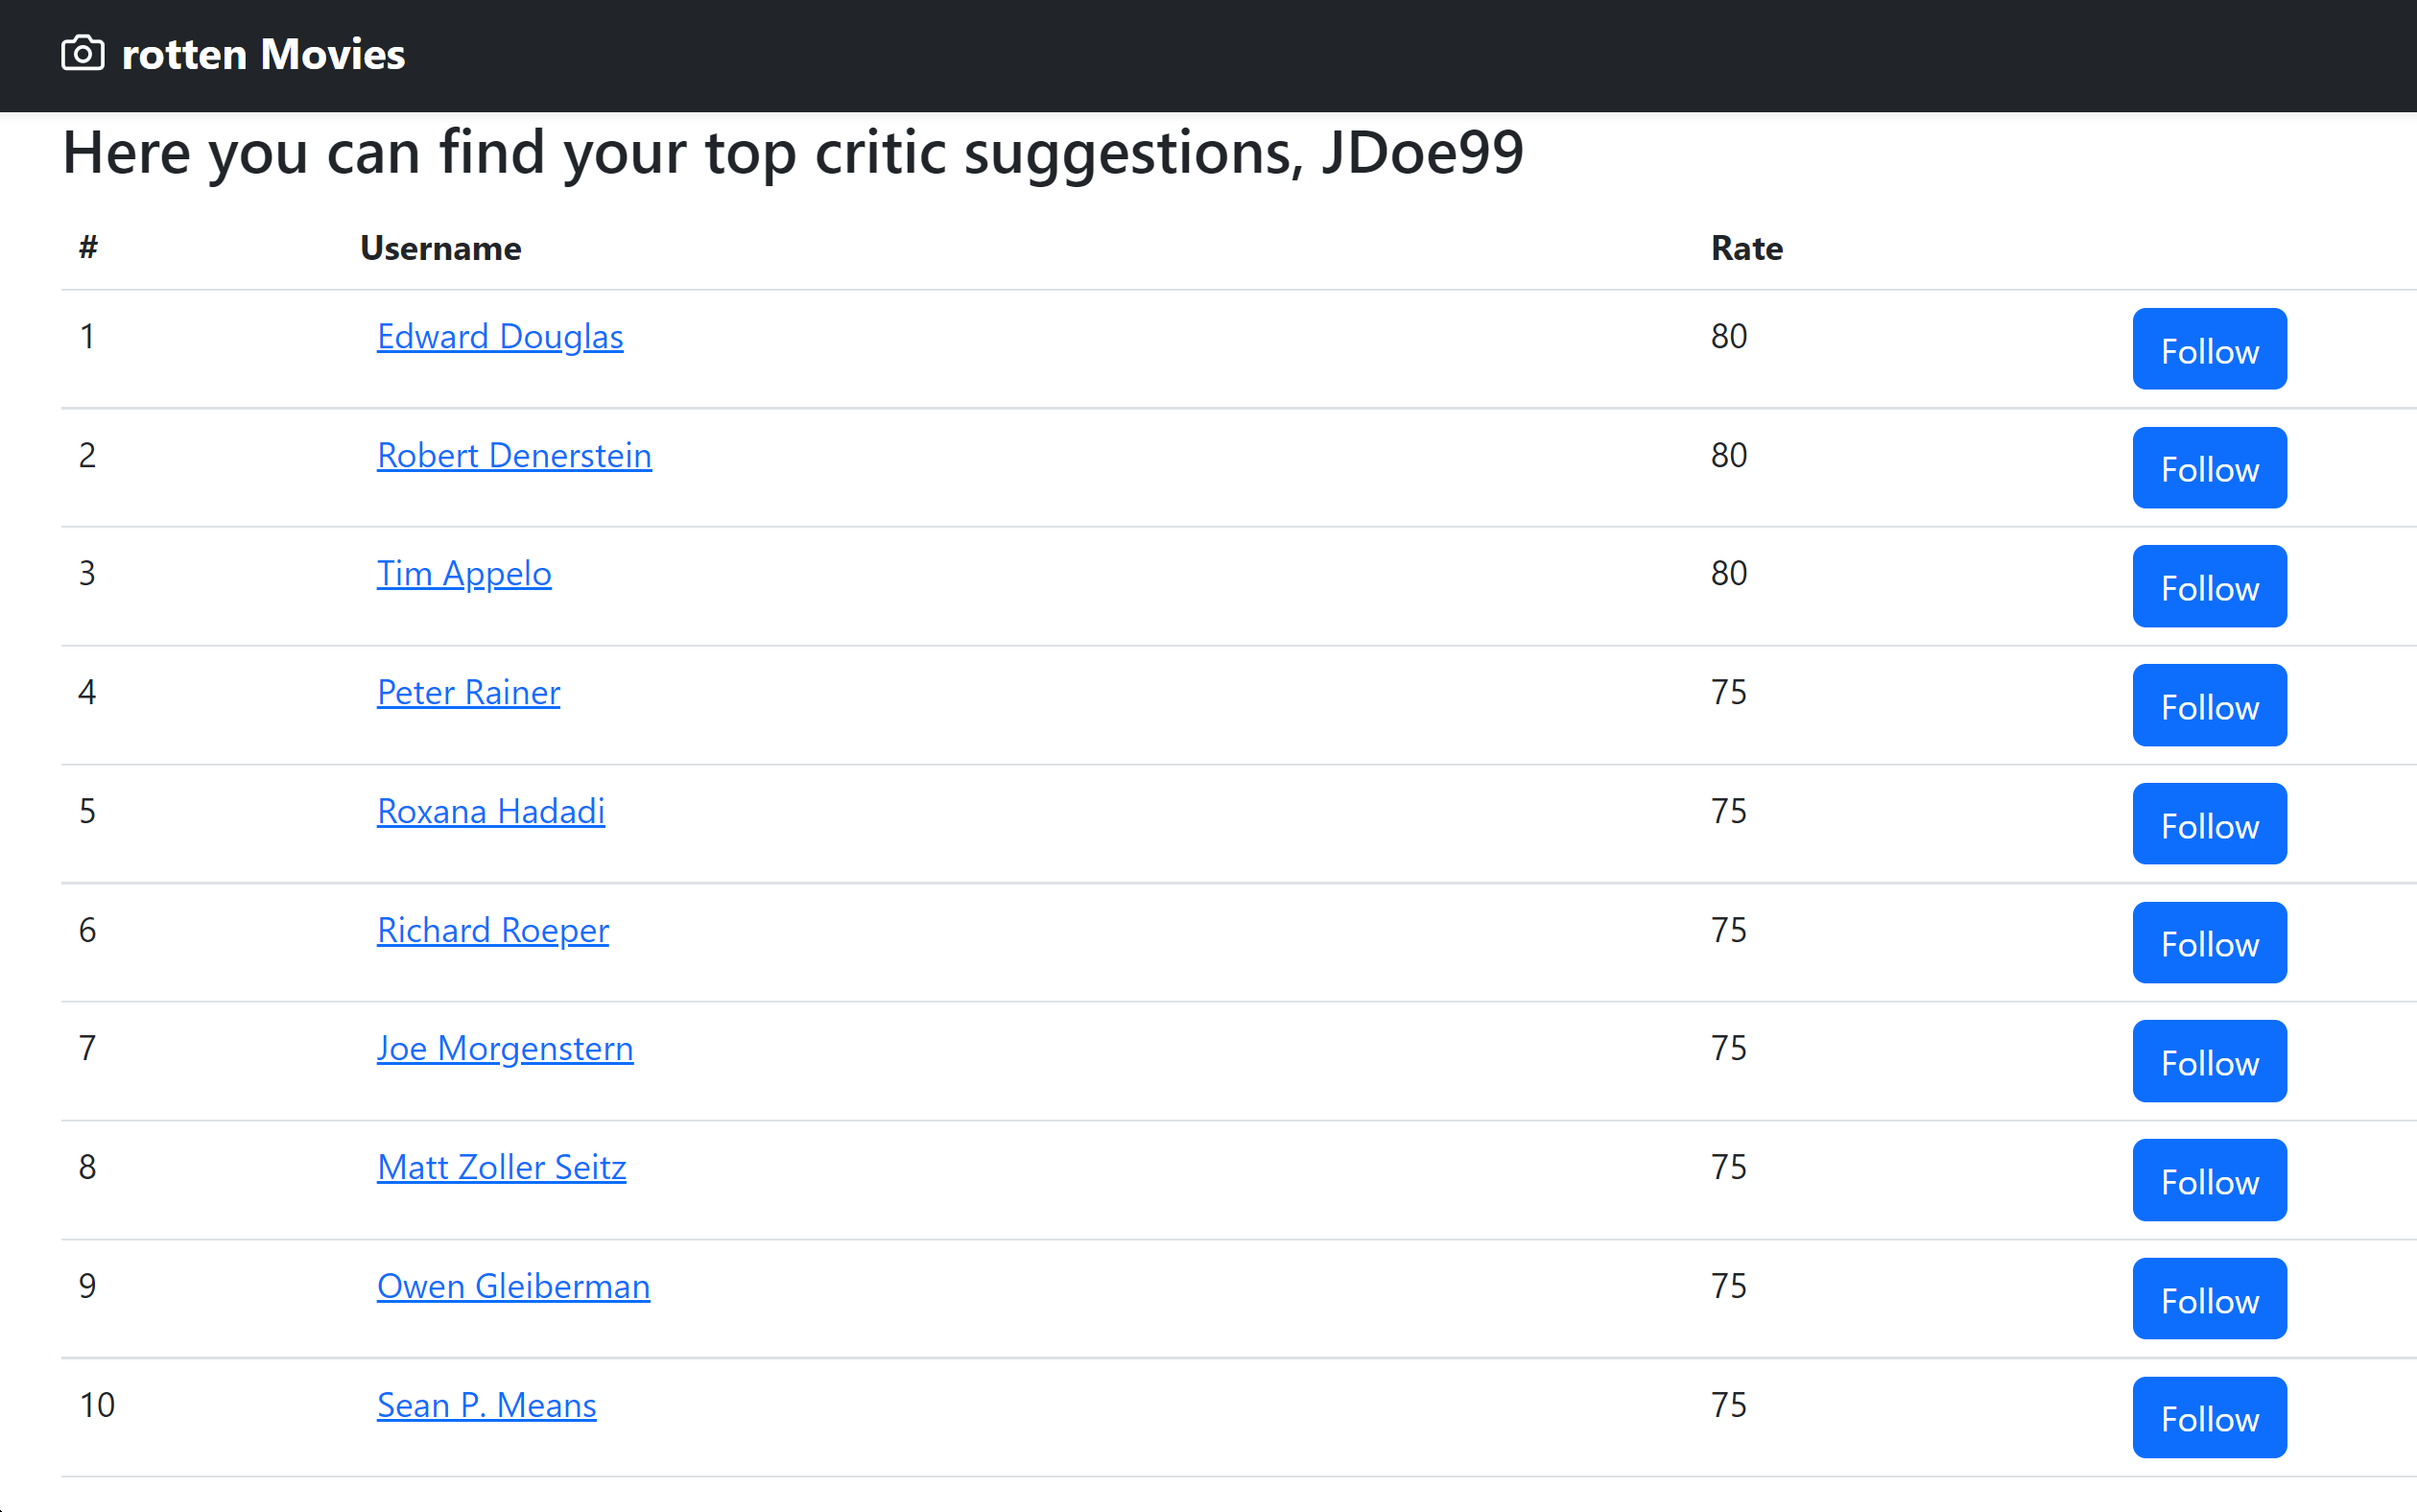
\includegraphics[scale=0.45]{../../../images/user_manual/suggestions.png} 
\end{center}
\vspace{5pt}

The suggestion page shows a list of possible top critics that the user could follow. These top critics are chosen based on common reviewed movies (both positively or both negatively) between the two. The Rate index shows the estimated probability that the user might align with the suggested top critic views.

\begin{center}
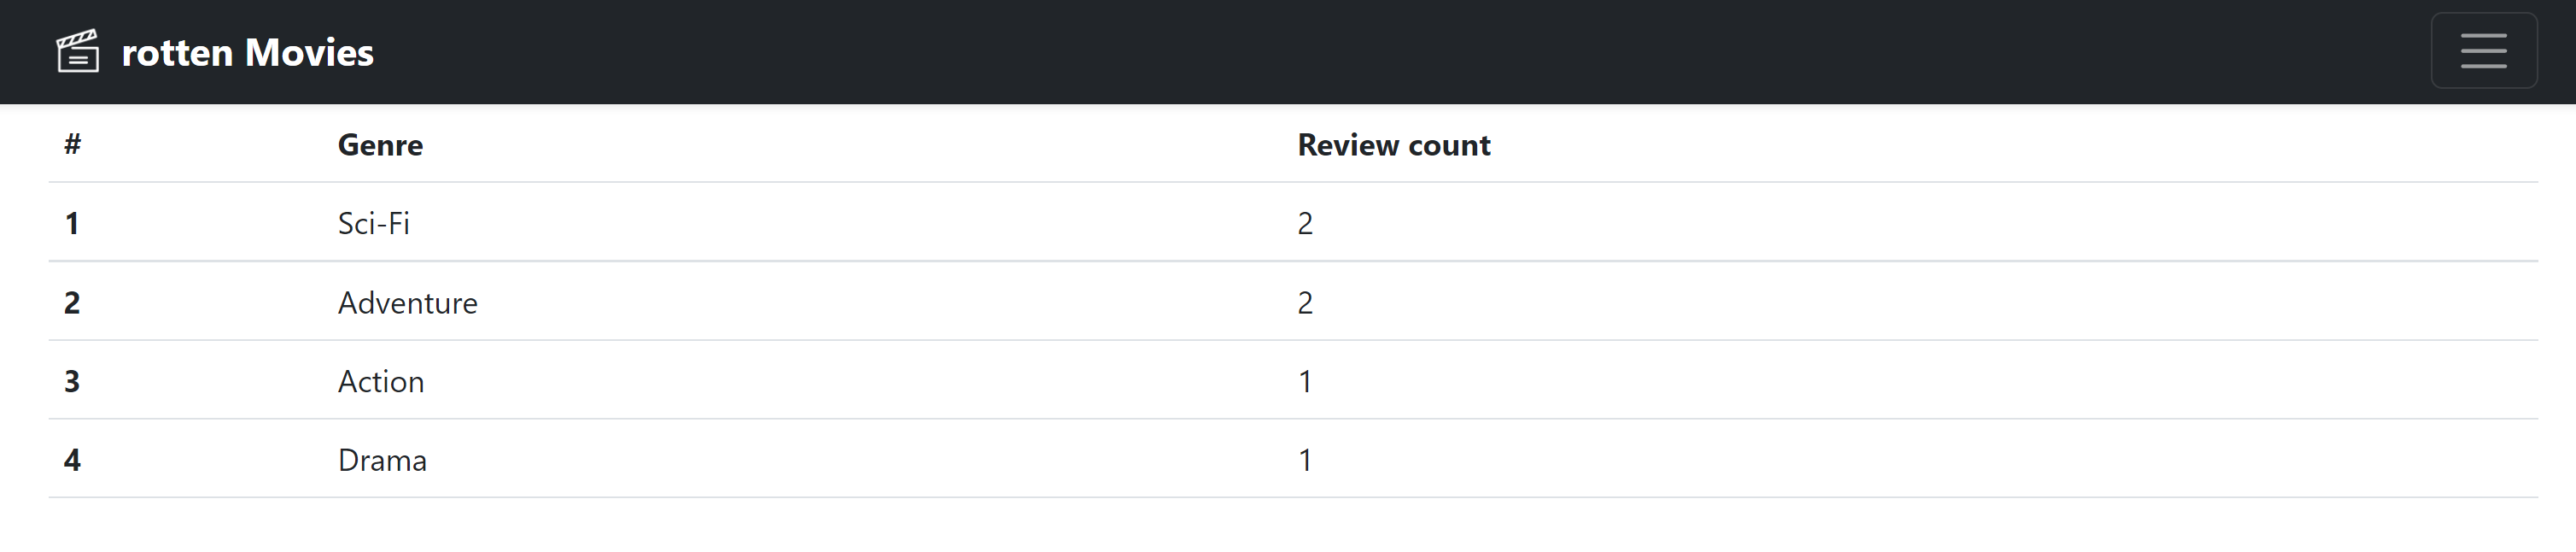
\includegraphics[scale=0.45]{../../../images/user_manual/preferred_genres.png}
\end{center}
\vspace{5pt}

The preferred genres page shows an aggregated overview of genres reviewed by the user. This highlights possible preferences towards certain genres more than others

\begin{center}
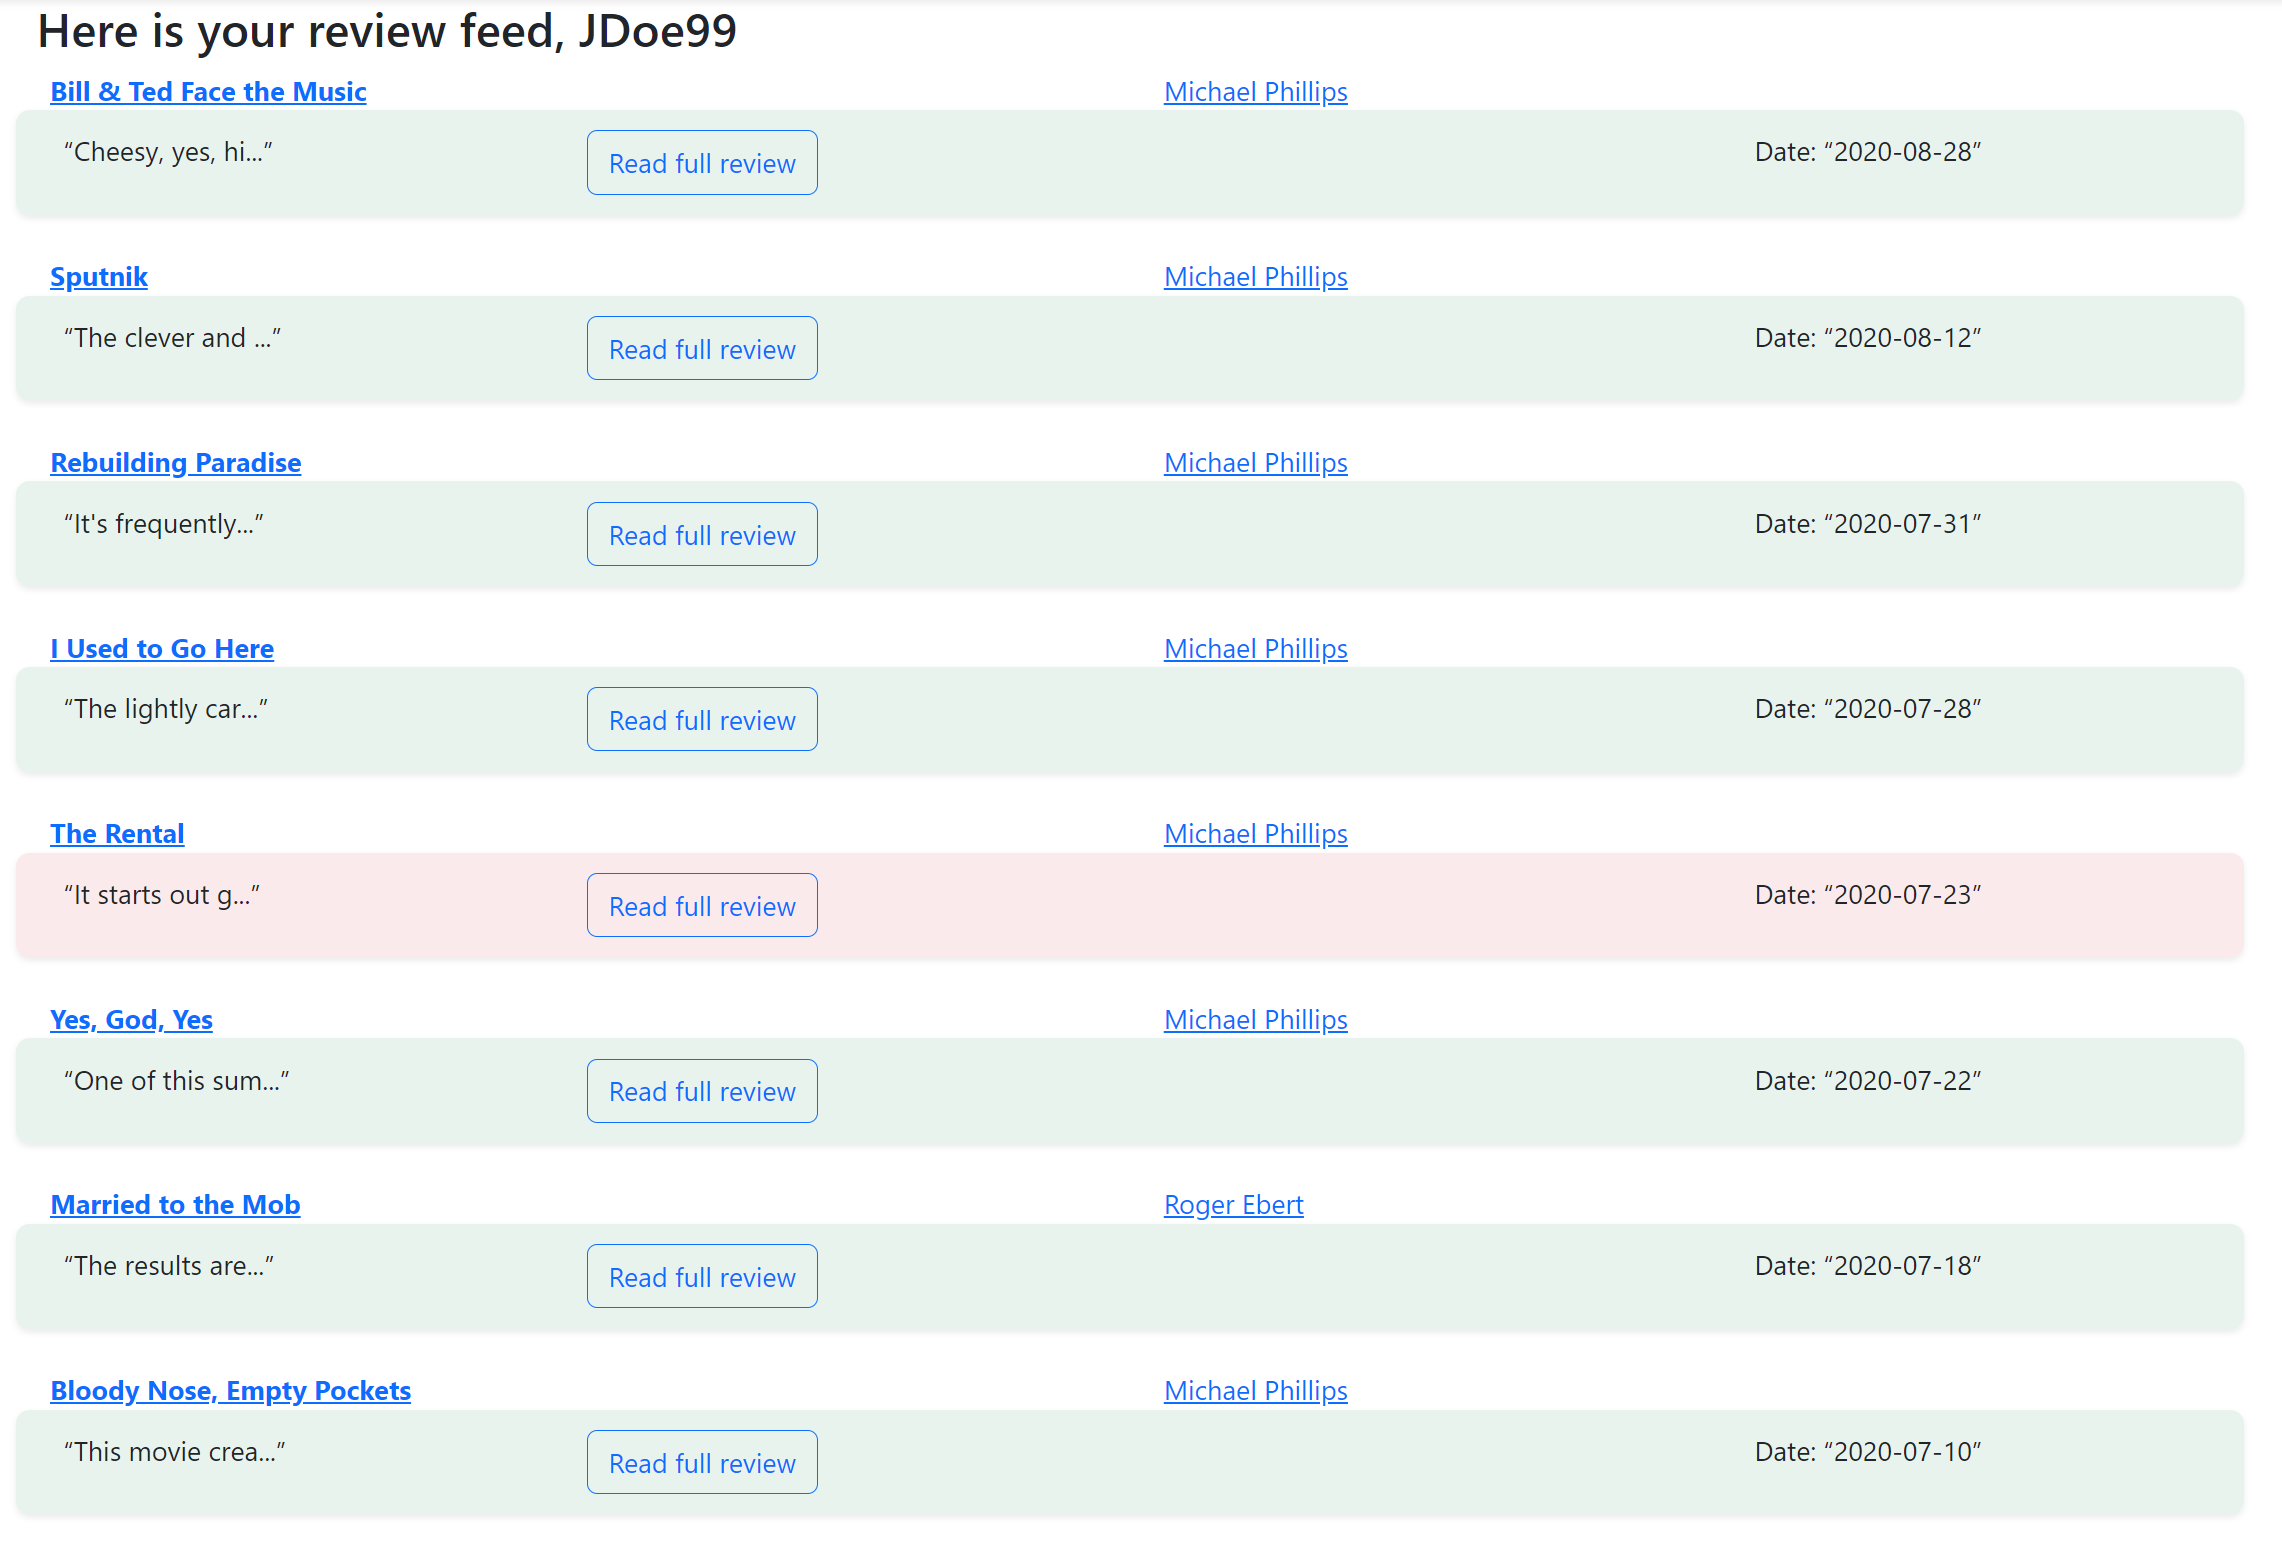
\includegraphics[scale=0.45]{../../../images/user_manual/feed.png} 
\end{center}
\vspace{5pt}

The feed shows a list of recent reviews written by followed top critics. The review contains an excerpt of the full content, which can be seen by clicking on the button \textit{Read full review}

\begin{center}
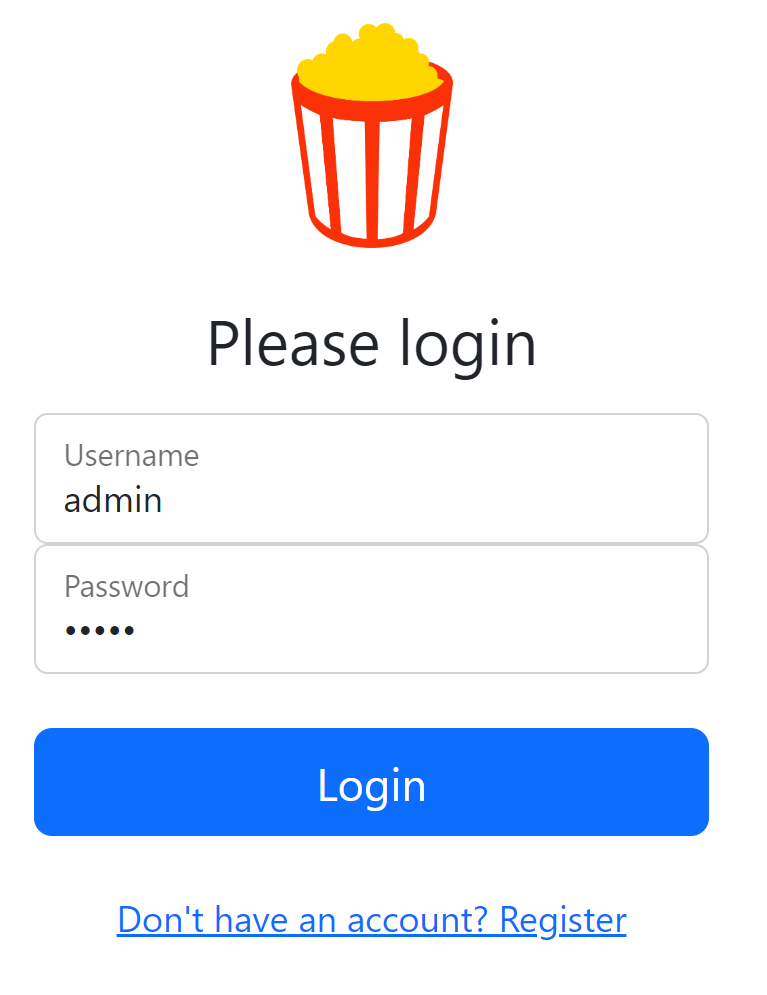
\includegraphics[scale=0.45]{../../../images/user_manual/admin_login.png} 
\end{center}
\vspace{5pt}

A special kind of user can log-in to perform administration tasks on the application

\begin{center}

\includegraphics[scale=0.45]{../../../images/user_manual/admin_navbar.png} 

\end{center}
\vspace{5pt}
The admin navbar allows to reach the administrator panel

\begin{center}
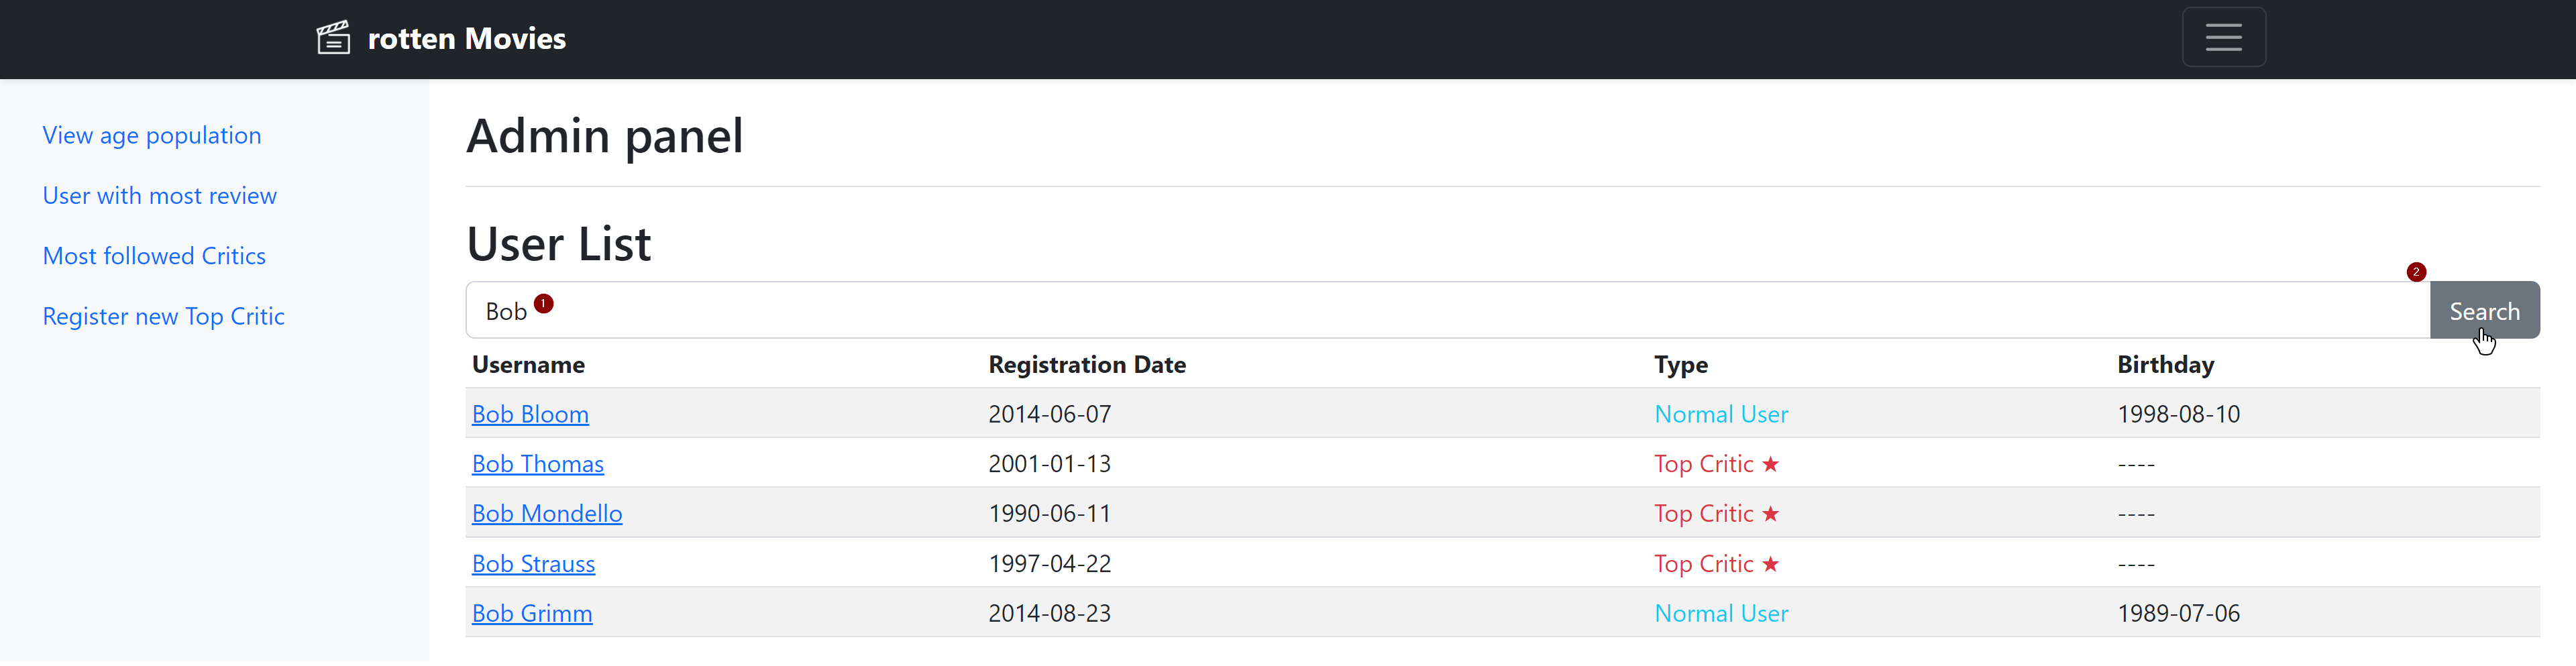
\includegraphics[scale=0.45]{../../../images/user_manual/admin_panel_search_user.png} 
\end{center}
\vspace{5pt}
In the administrator panel the admin can search for a specific user. The side panel links to different analytic pages about the status of the application

\begin{center}
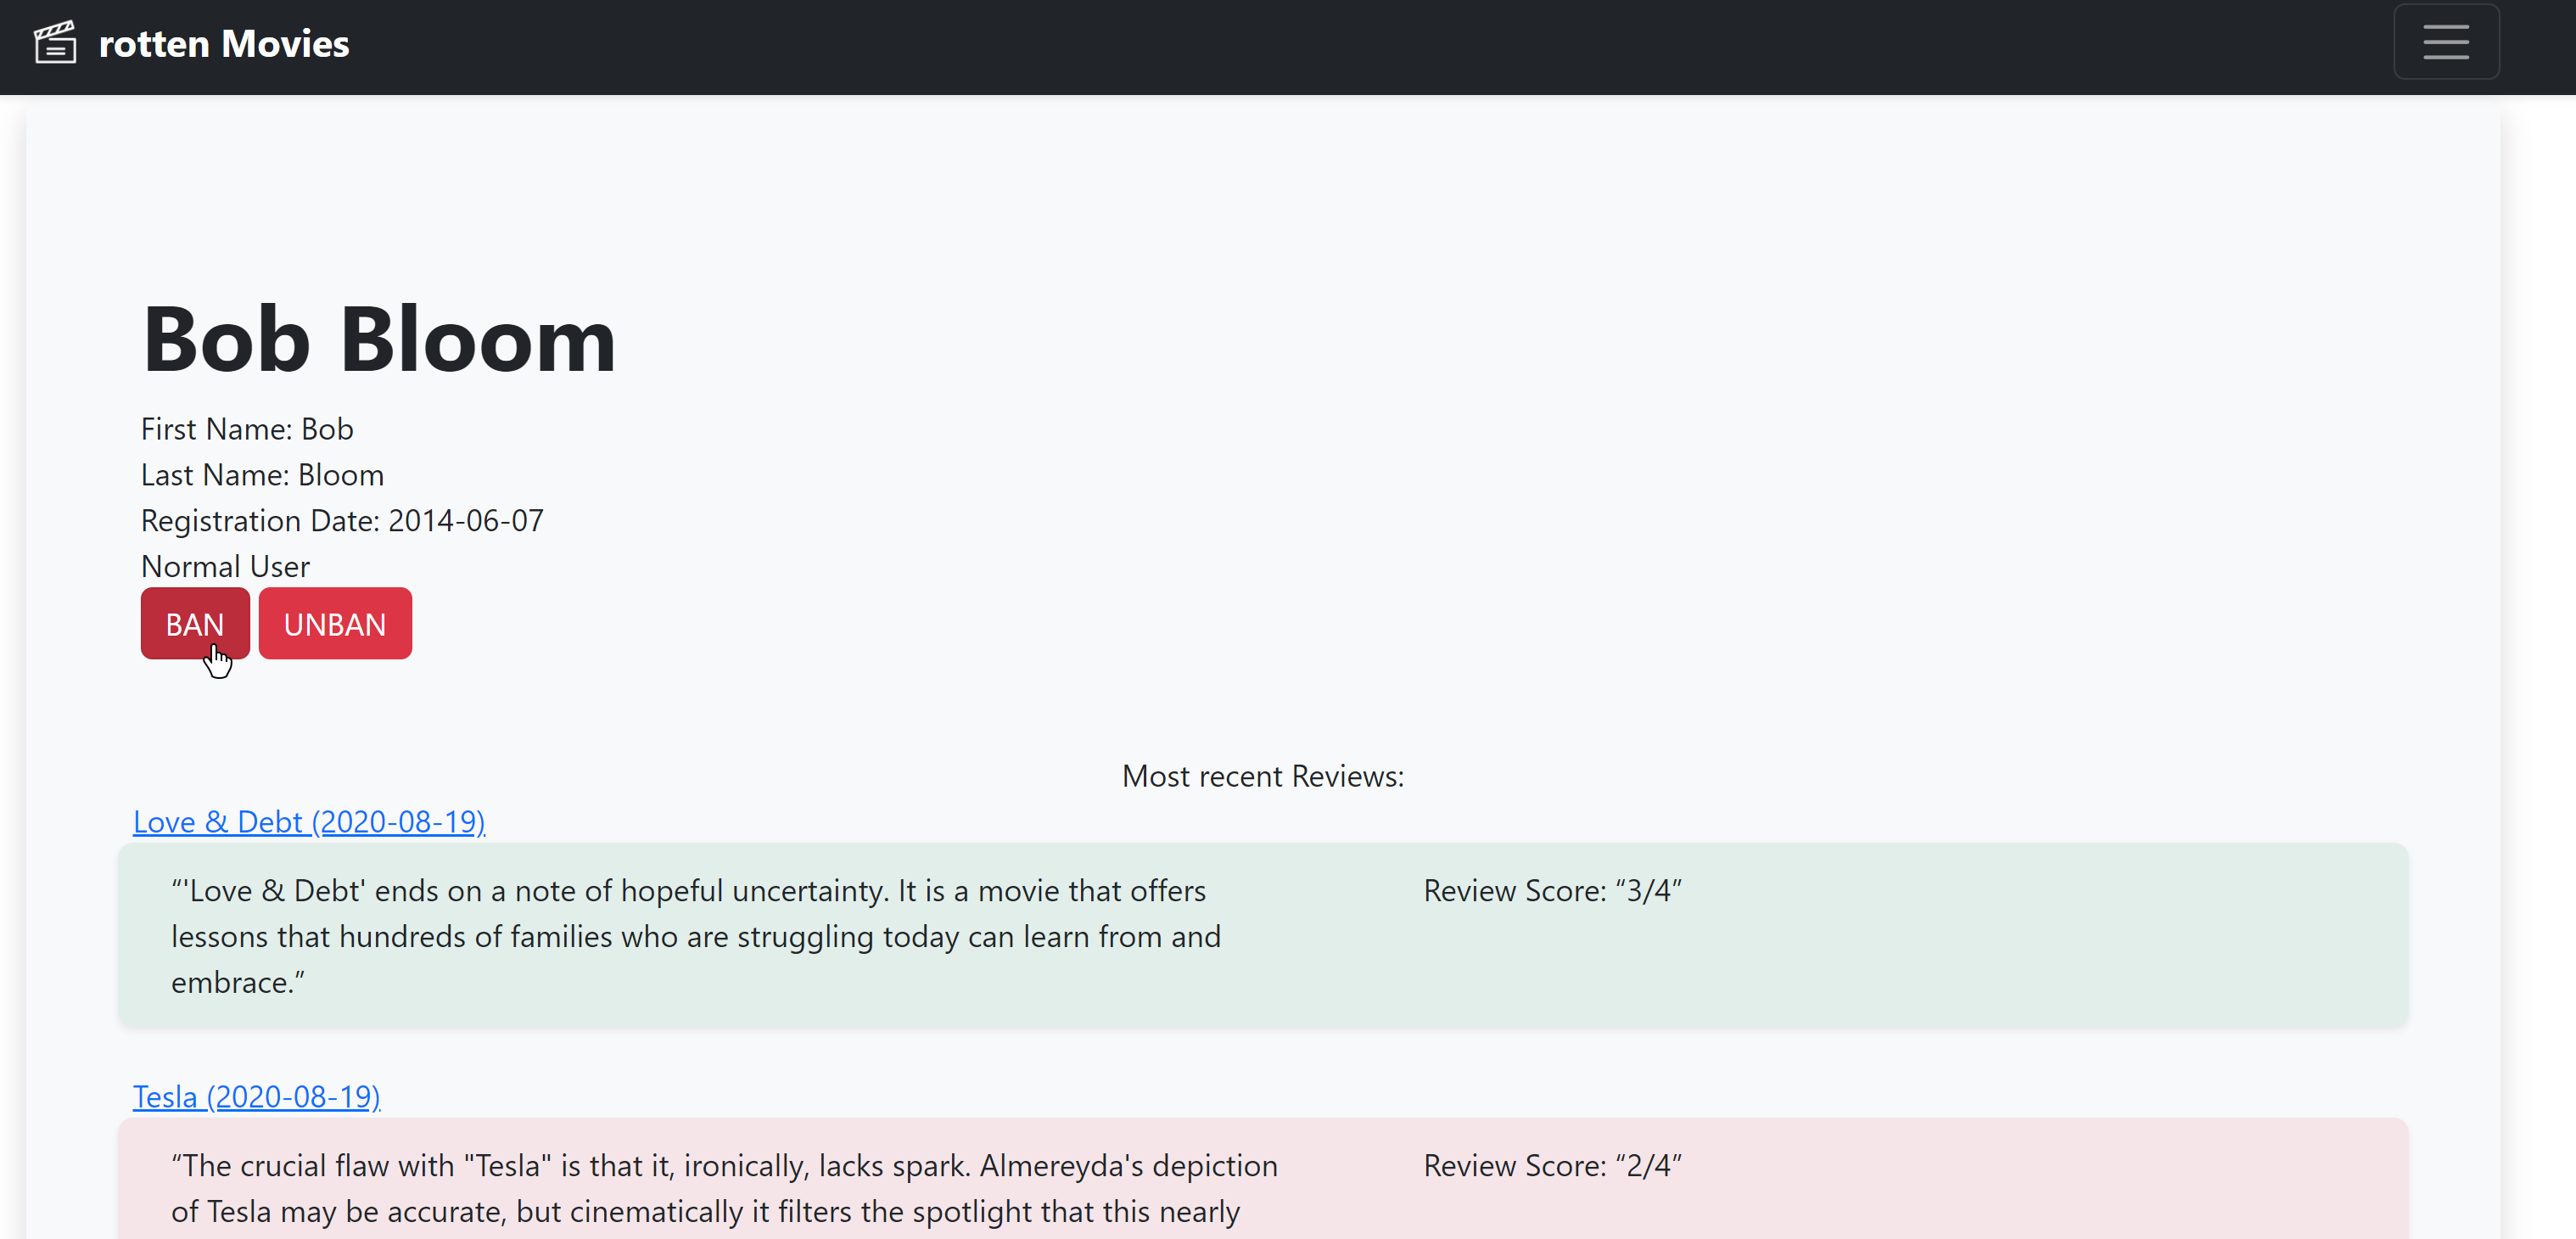
\includegraphics[scale=0.45]{../../../images/user_manual/ban_user.png} 
\end{center}
\vspace{5pt}

After selecting a user, the admin can ban or unban it

\begin{center}
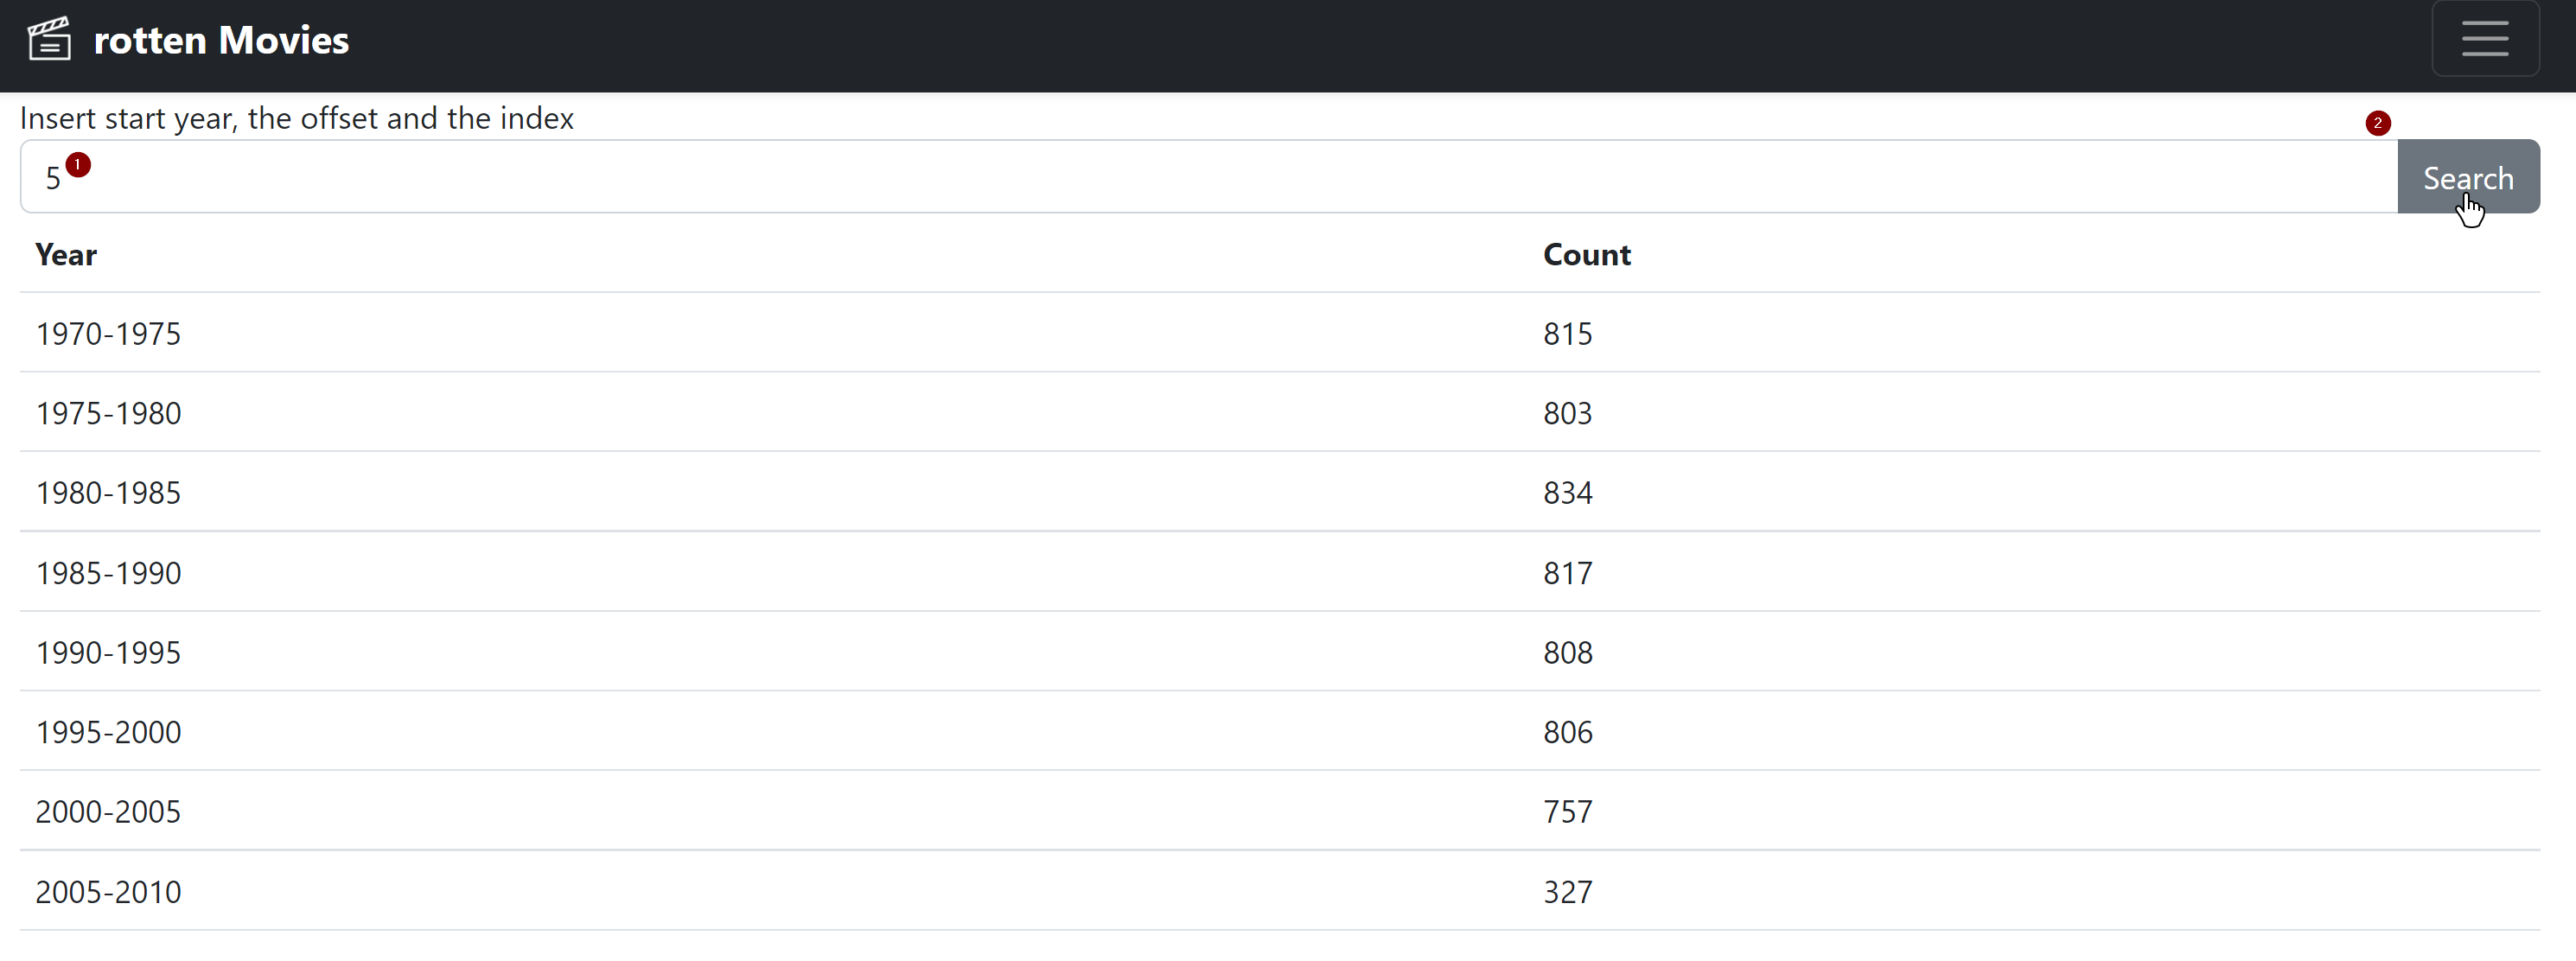
\includegraphics[scale=0.45]{../../../images/user_manual/population_by_age.png} 

\end{center}
\vspace{5pt}
This analytic shows the number of registered users for each year range, passed as input

\begin{center}
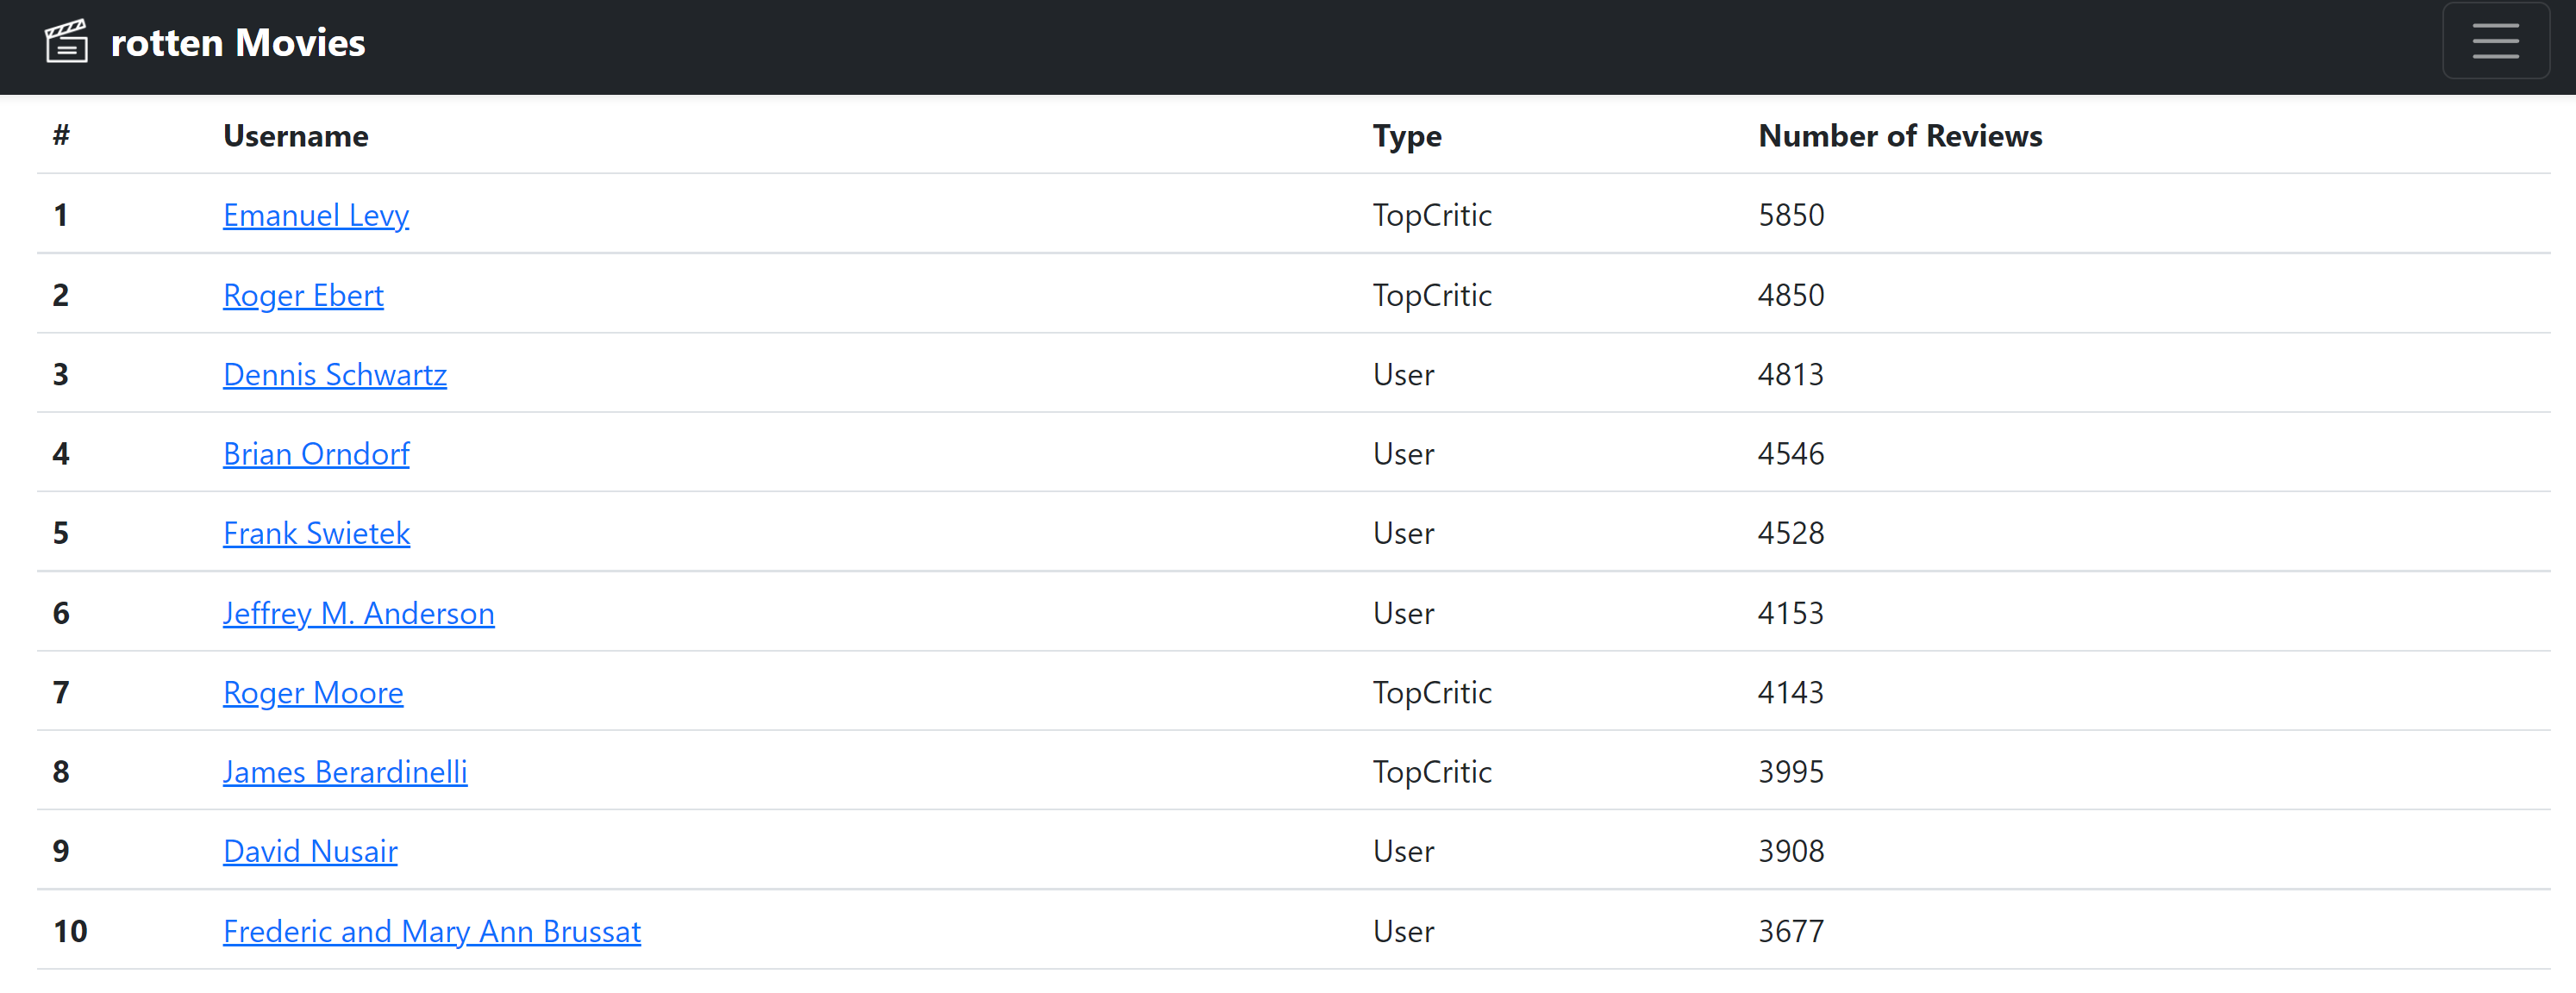
\includegraphics[scale=0.45]{../../../images/user_manual/most_active_users.png} 

\end{center}
\vspace{5pt}

This page shows a ranking of users based on their number of reviews. This can be useful to verify a possible automated user, or promote a certified active user as a top critic

\begin{center}
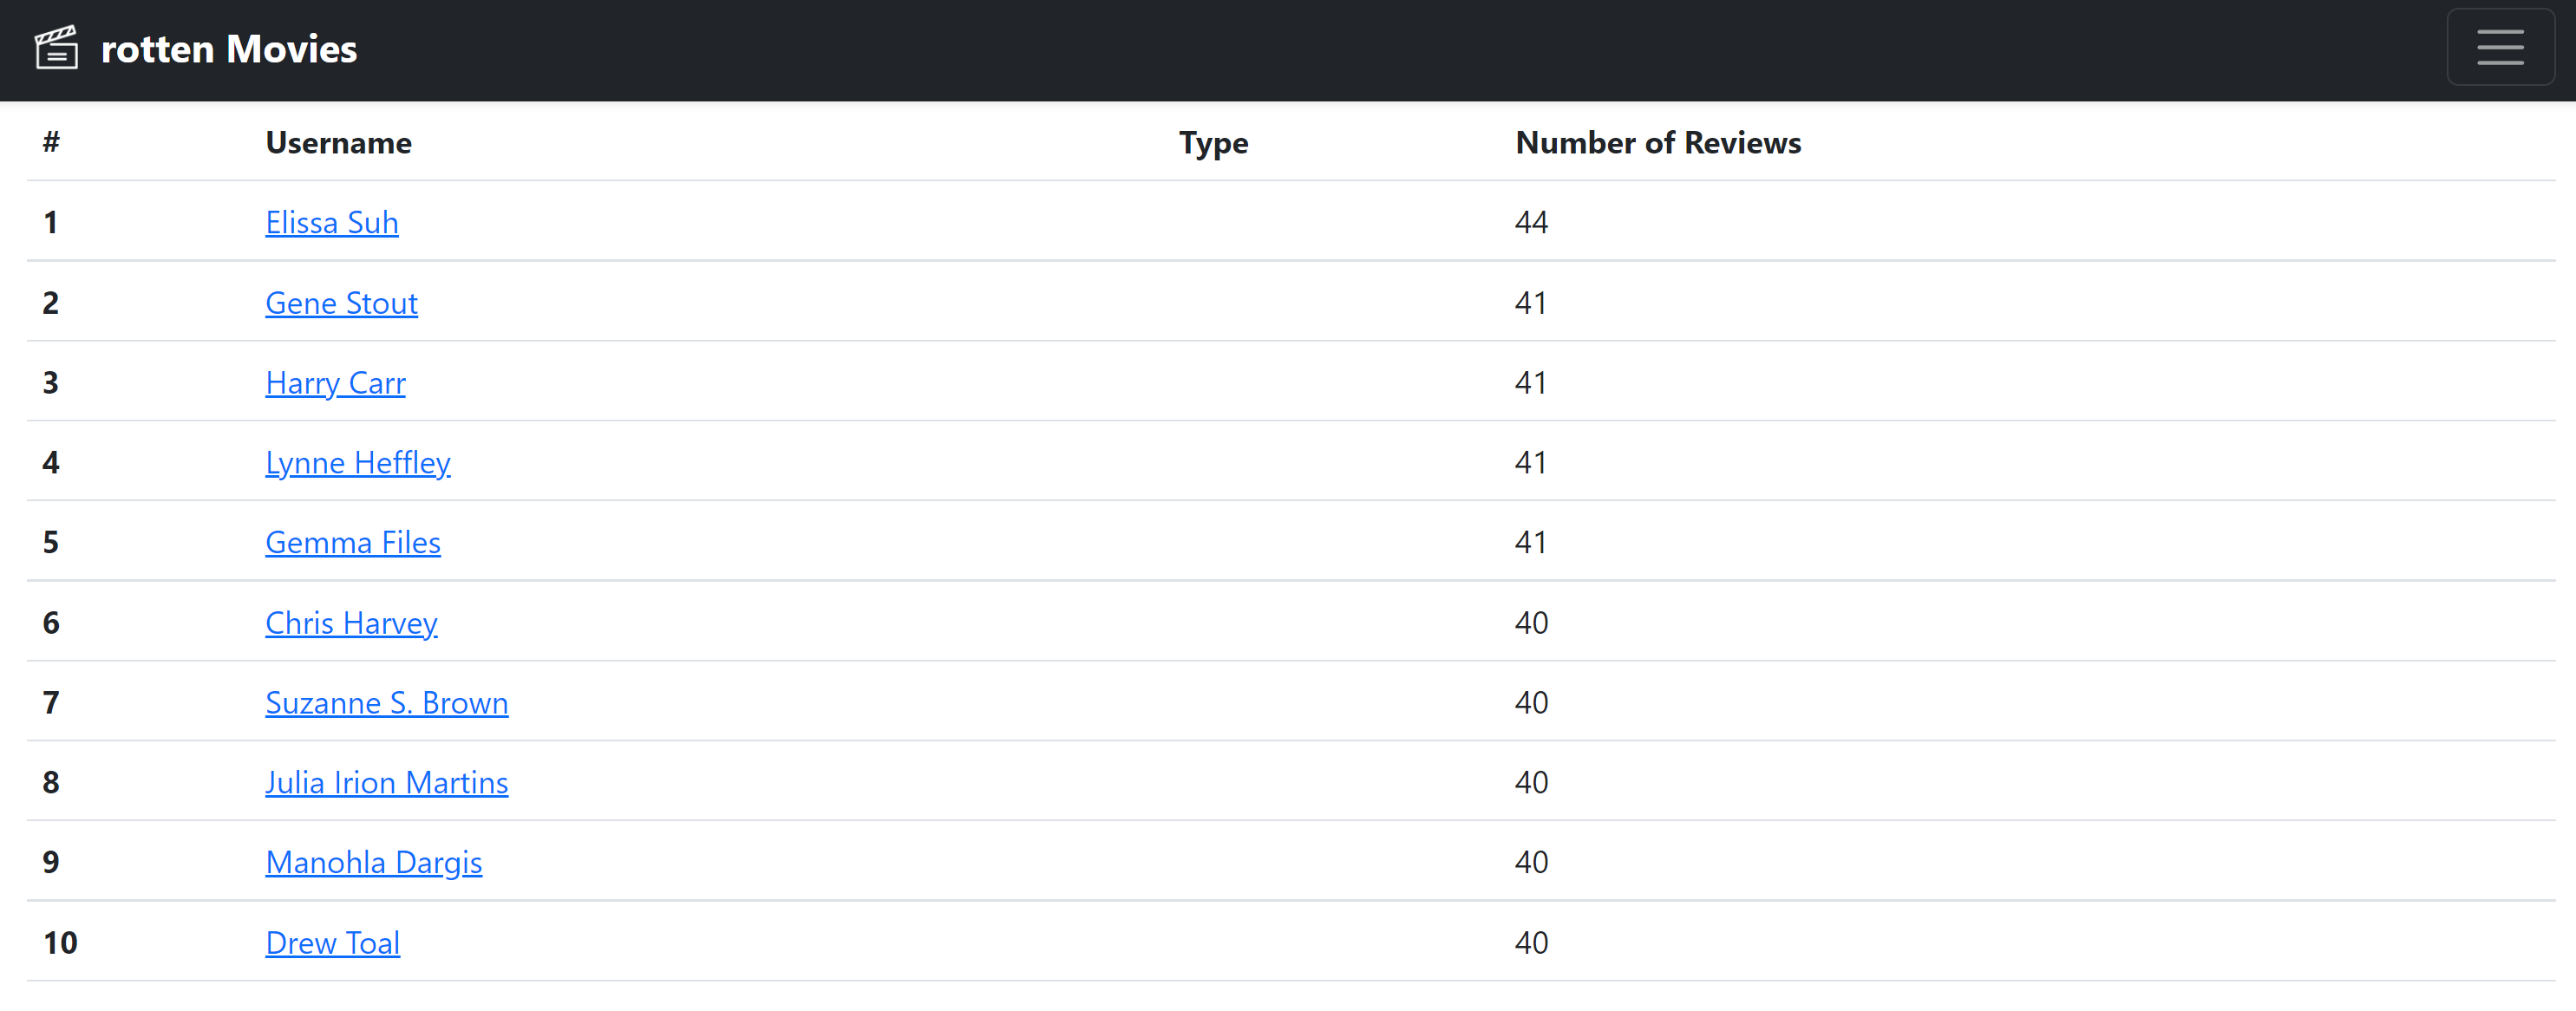
\includegraphics[scale=0.45]{../../../images/user_manual/most_followed_top_critic.png} 

\end{center}
\vspace{5pt}
With this page, the administrator can see a ranking of most active top critics, based on the number of reviews

\begin{center}
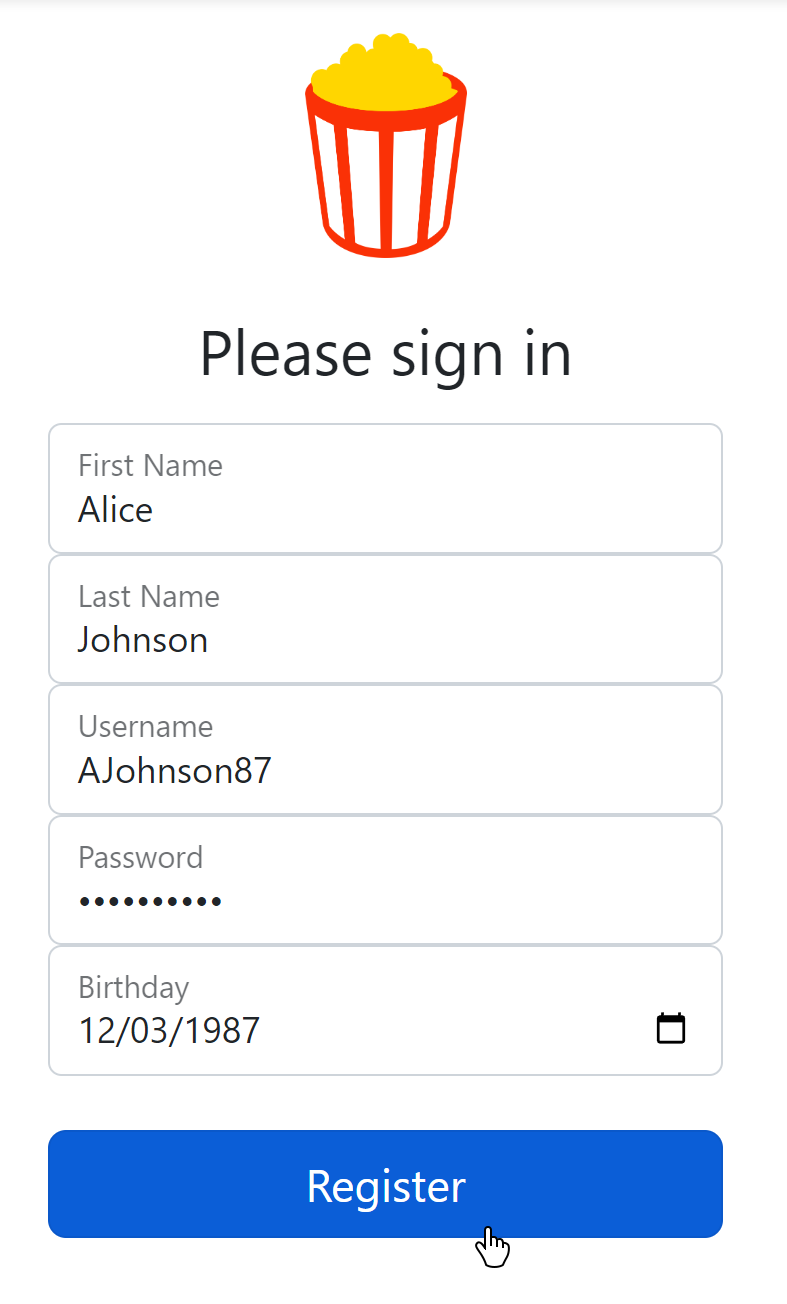
\includegraphics[scale=0.45]{../../../images/user_manual/top_critic_registration.png} 

\end{center}
\vspace{5pt}

The top critic creation page isn't accessible to the public, only to the registered administrator. It is very similar to the user registration page, but it doesn't redirect to the explore movie page after a successful sign-up

\begin{center}
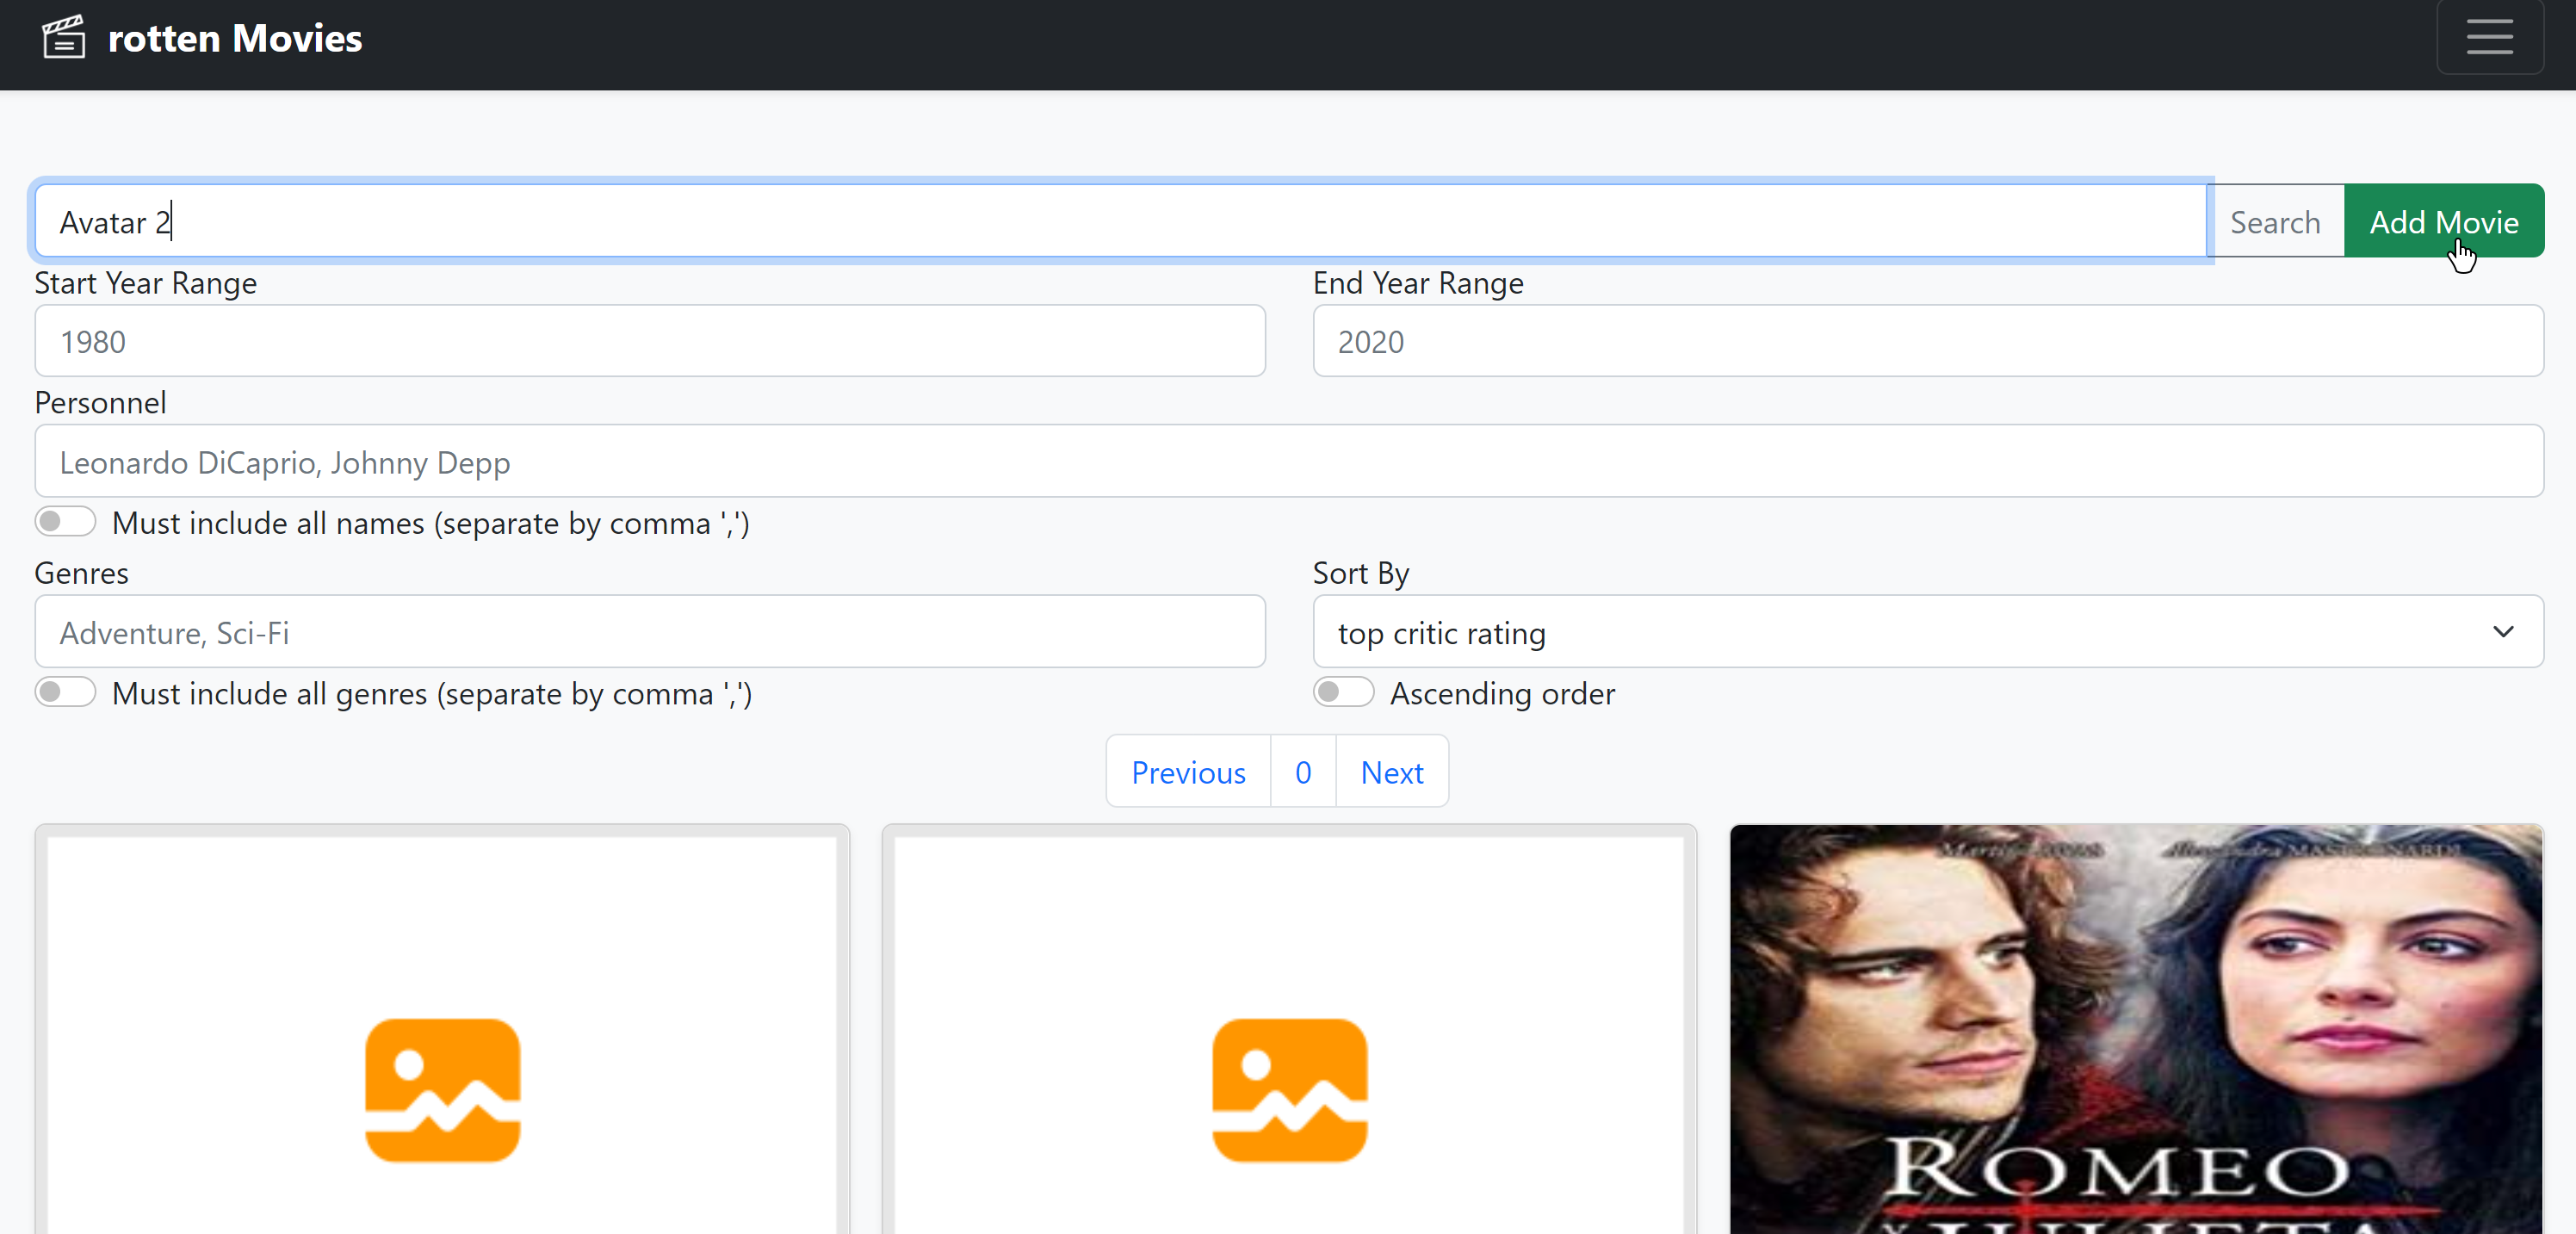
\includegraphics[scale=0.45]{../../../images/user_manual/add_new_movie.png} 

\end{center}
\vspace{5pt}

Adding a new movie is done through the explore movie page. A new button labeled \textit{Add Movie} appears near the \textit{Search} one and will create a new movie, temporarily named as the string currently present in the search bar

\begin{center}
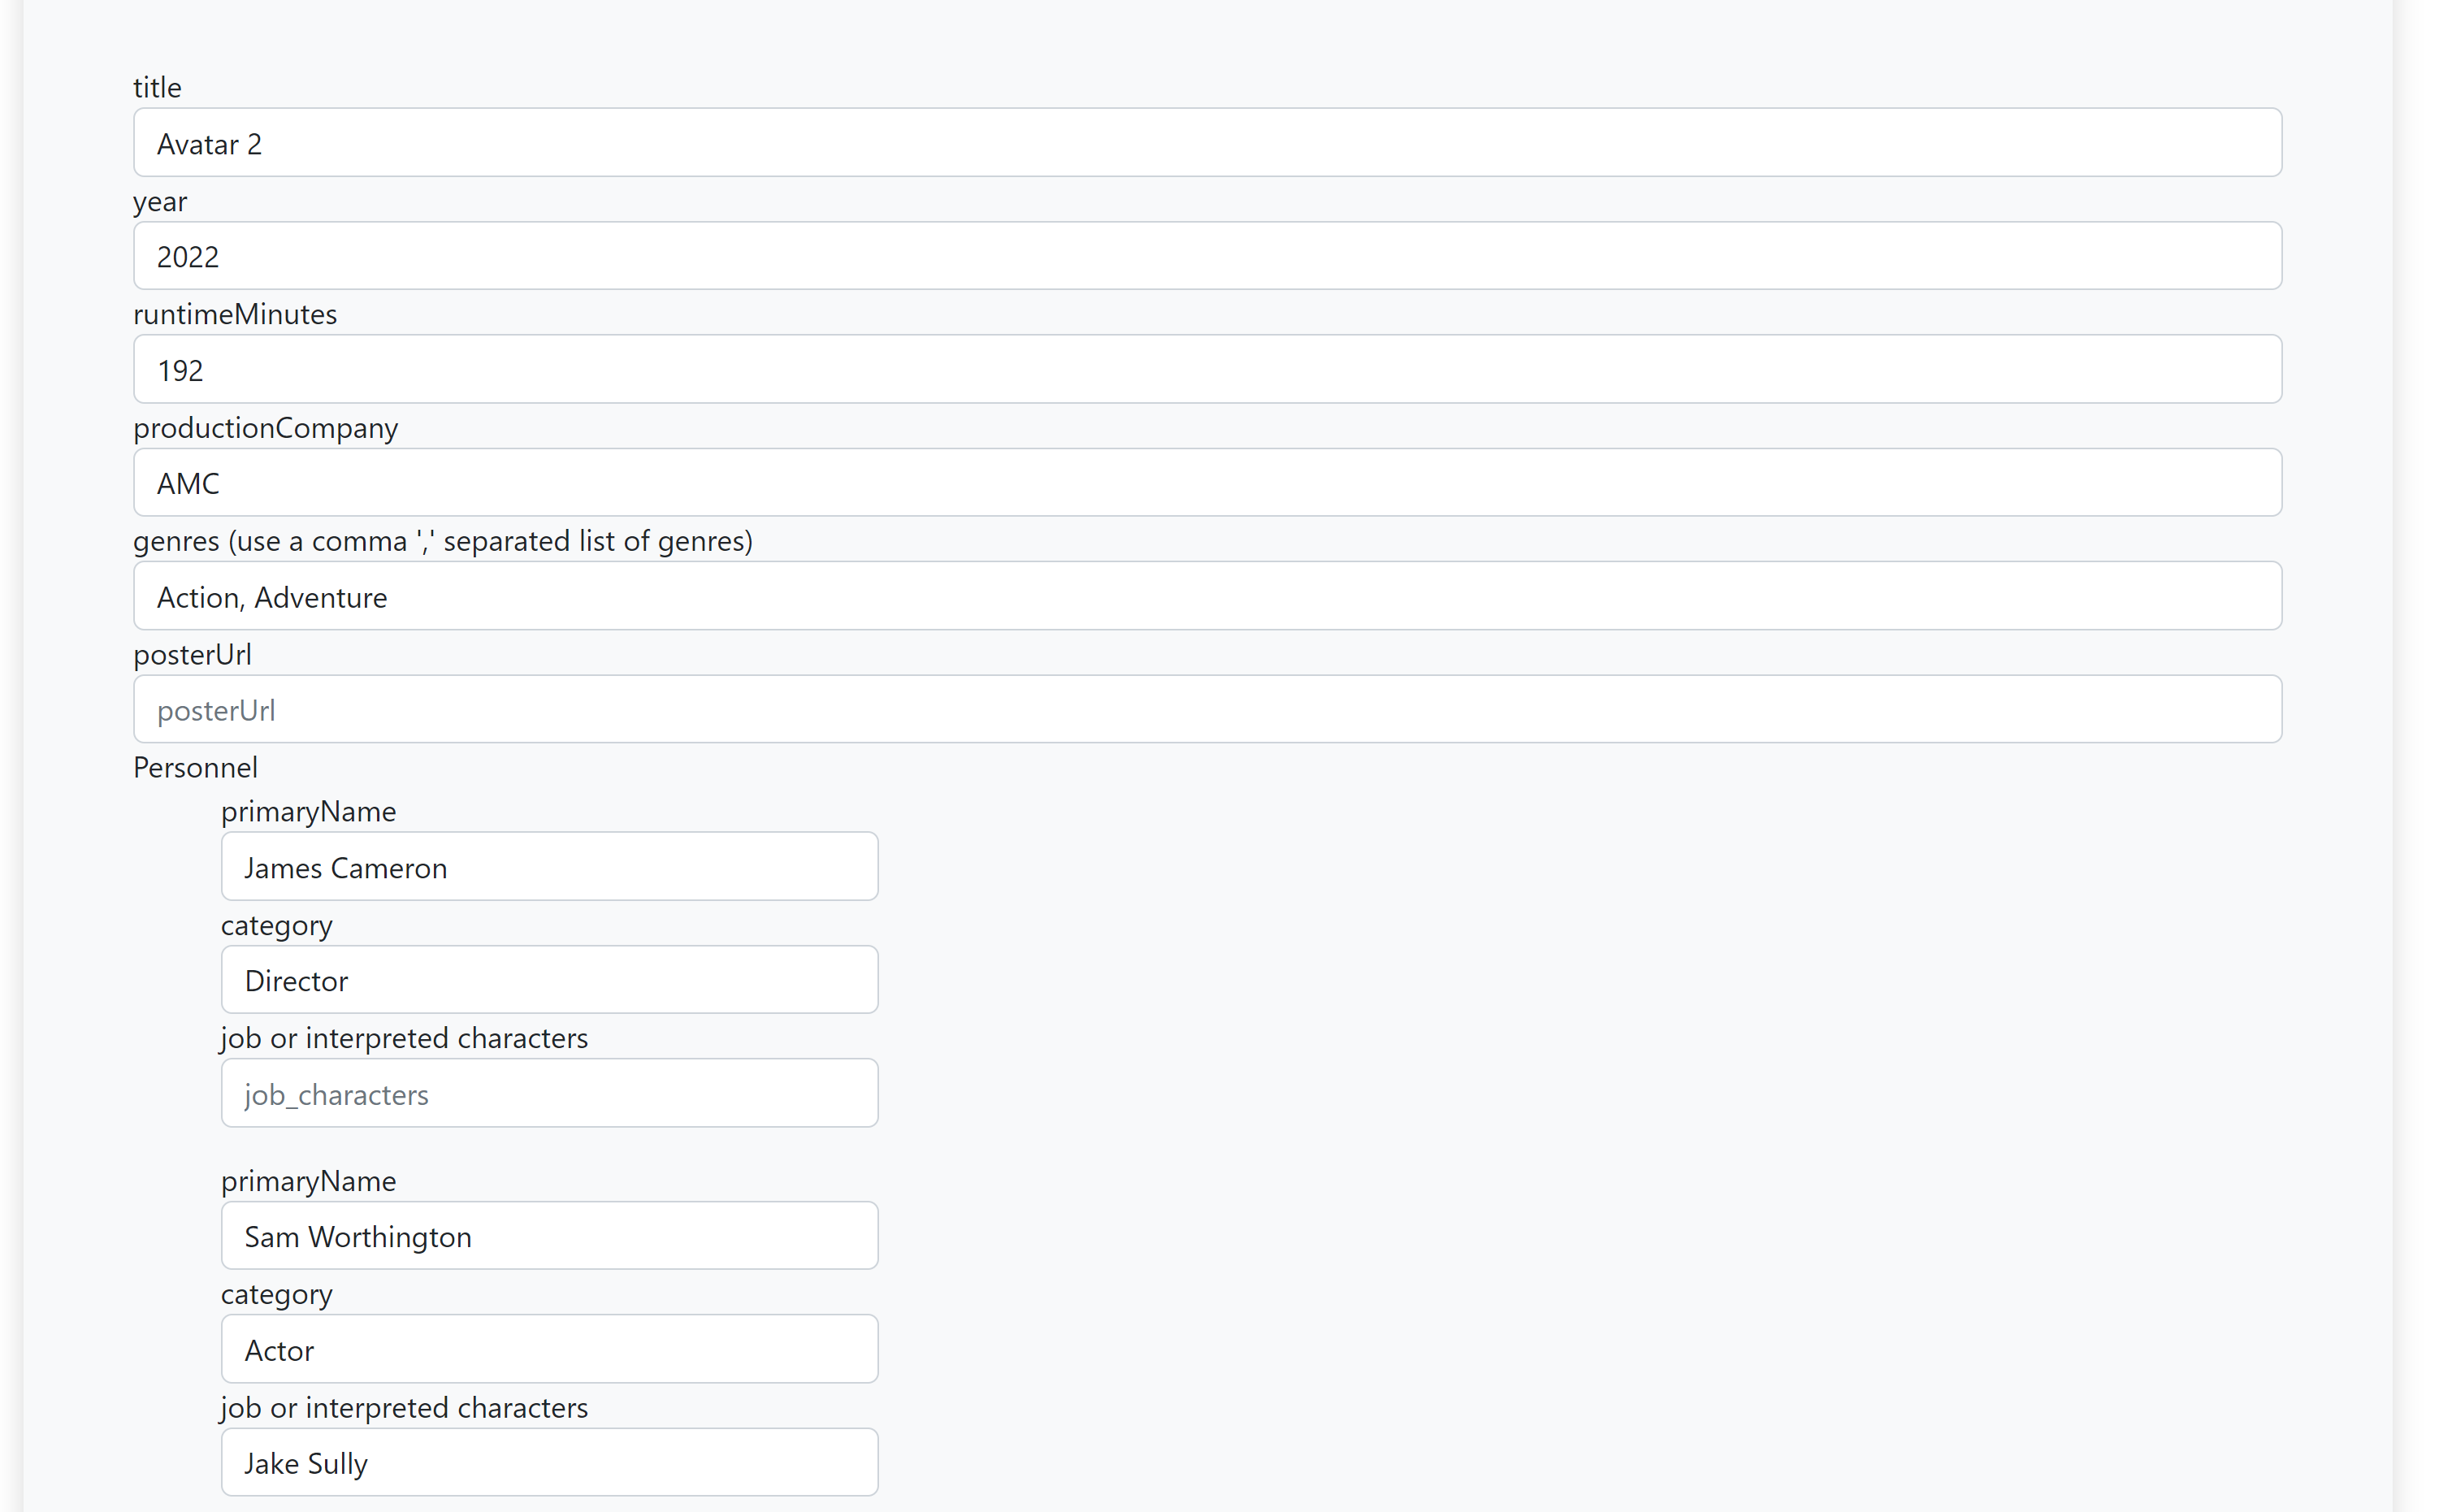
\includegraphics[scale=0.45]{../../../images/user_manual/movie_update.png} 

\end{center}
\vspace{5pt}
After adding a movie, or when selecting an existing one, the administrator can change its descriptive information

\begin{center}
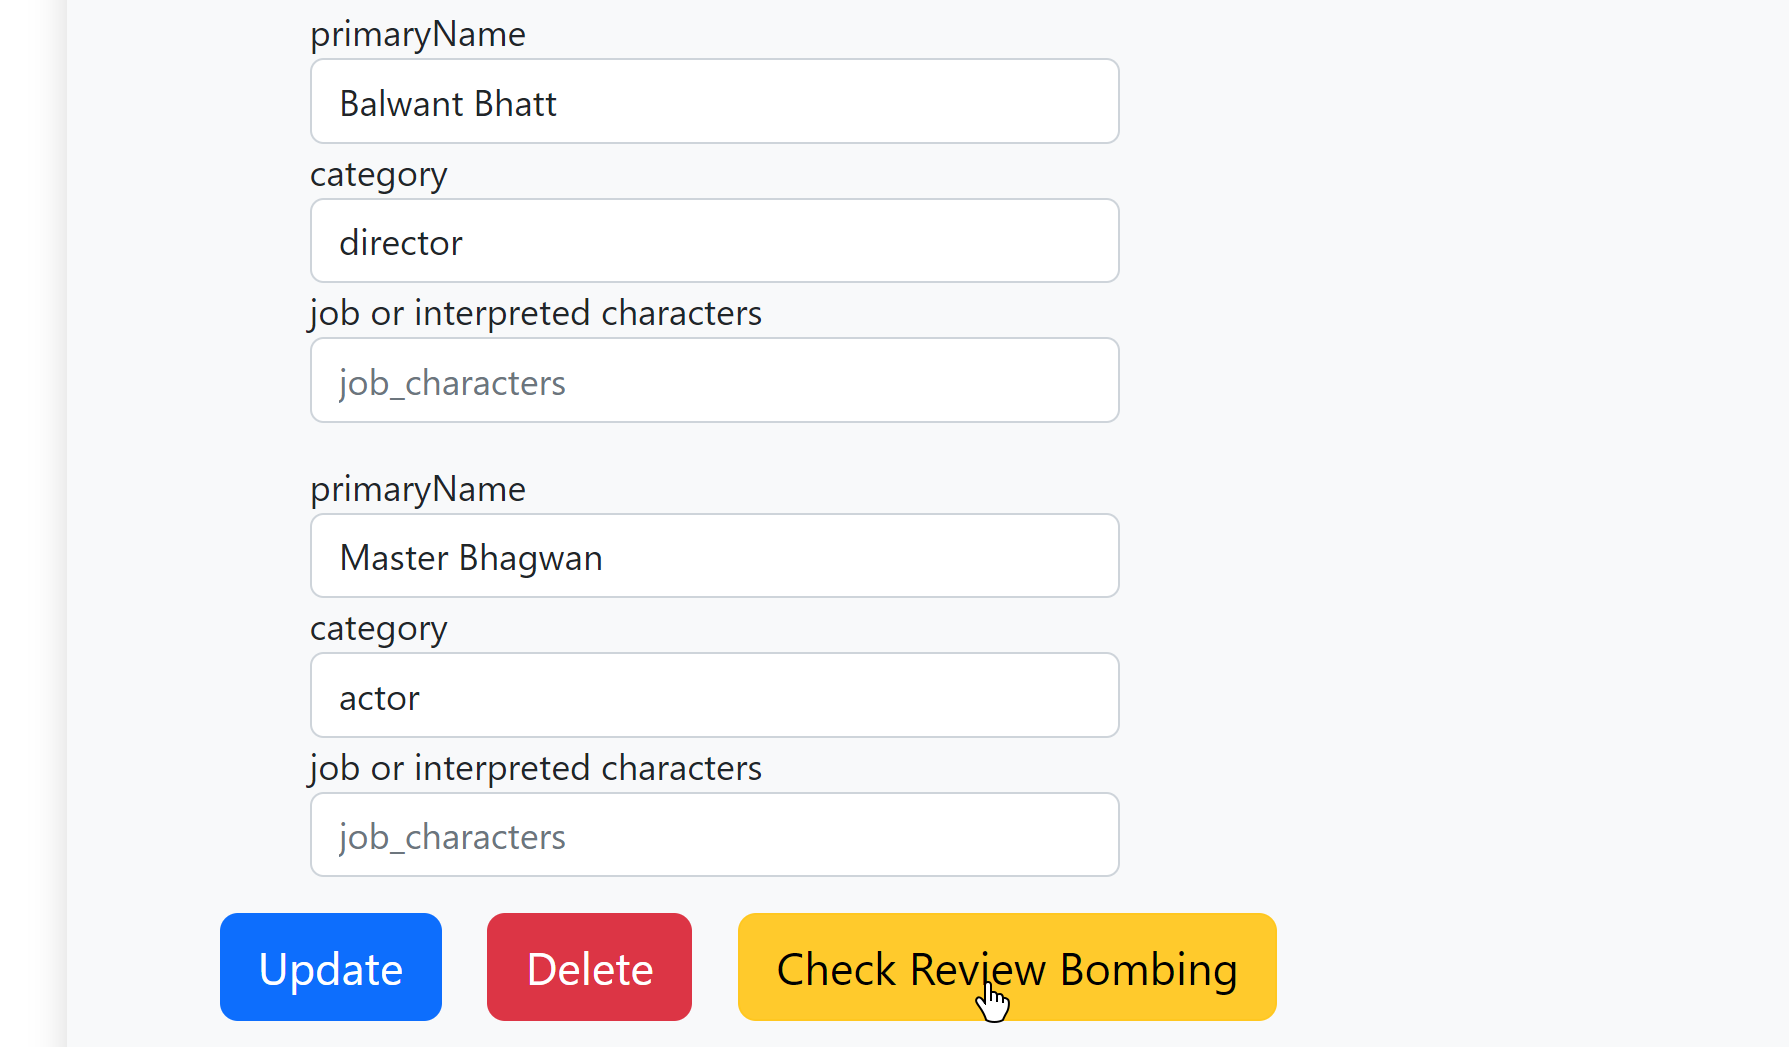
\includegraphics[scale=0.45]{../../../images/user_manual/check_review_bombing.png} 

\end{center}
\vspace{5pt}
When viewing a movie, the administrator can check for possible review bombing for this movie, by clicking on the specific button

\begin{center}
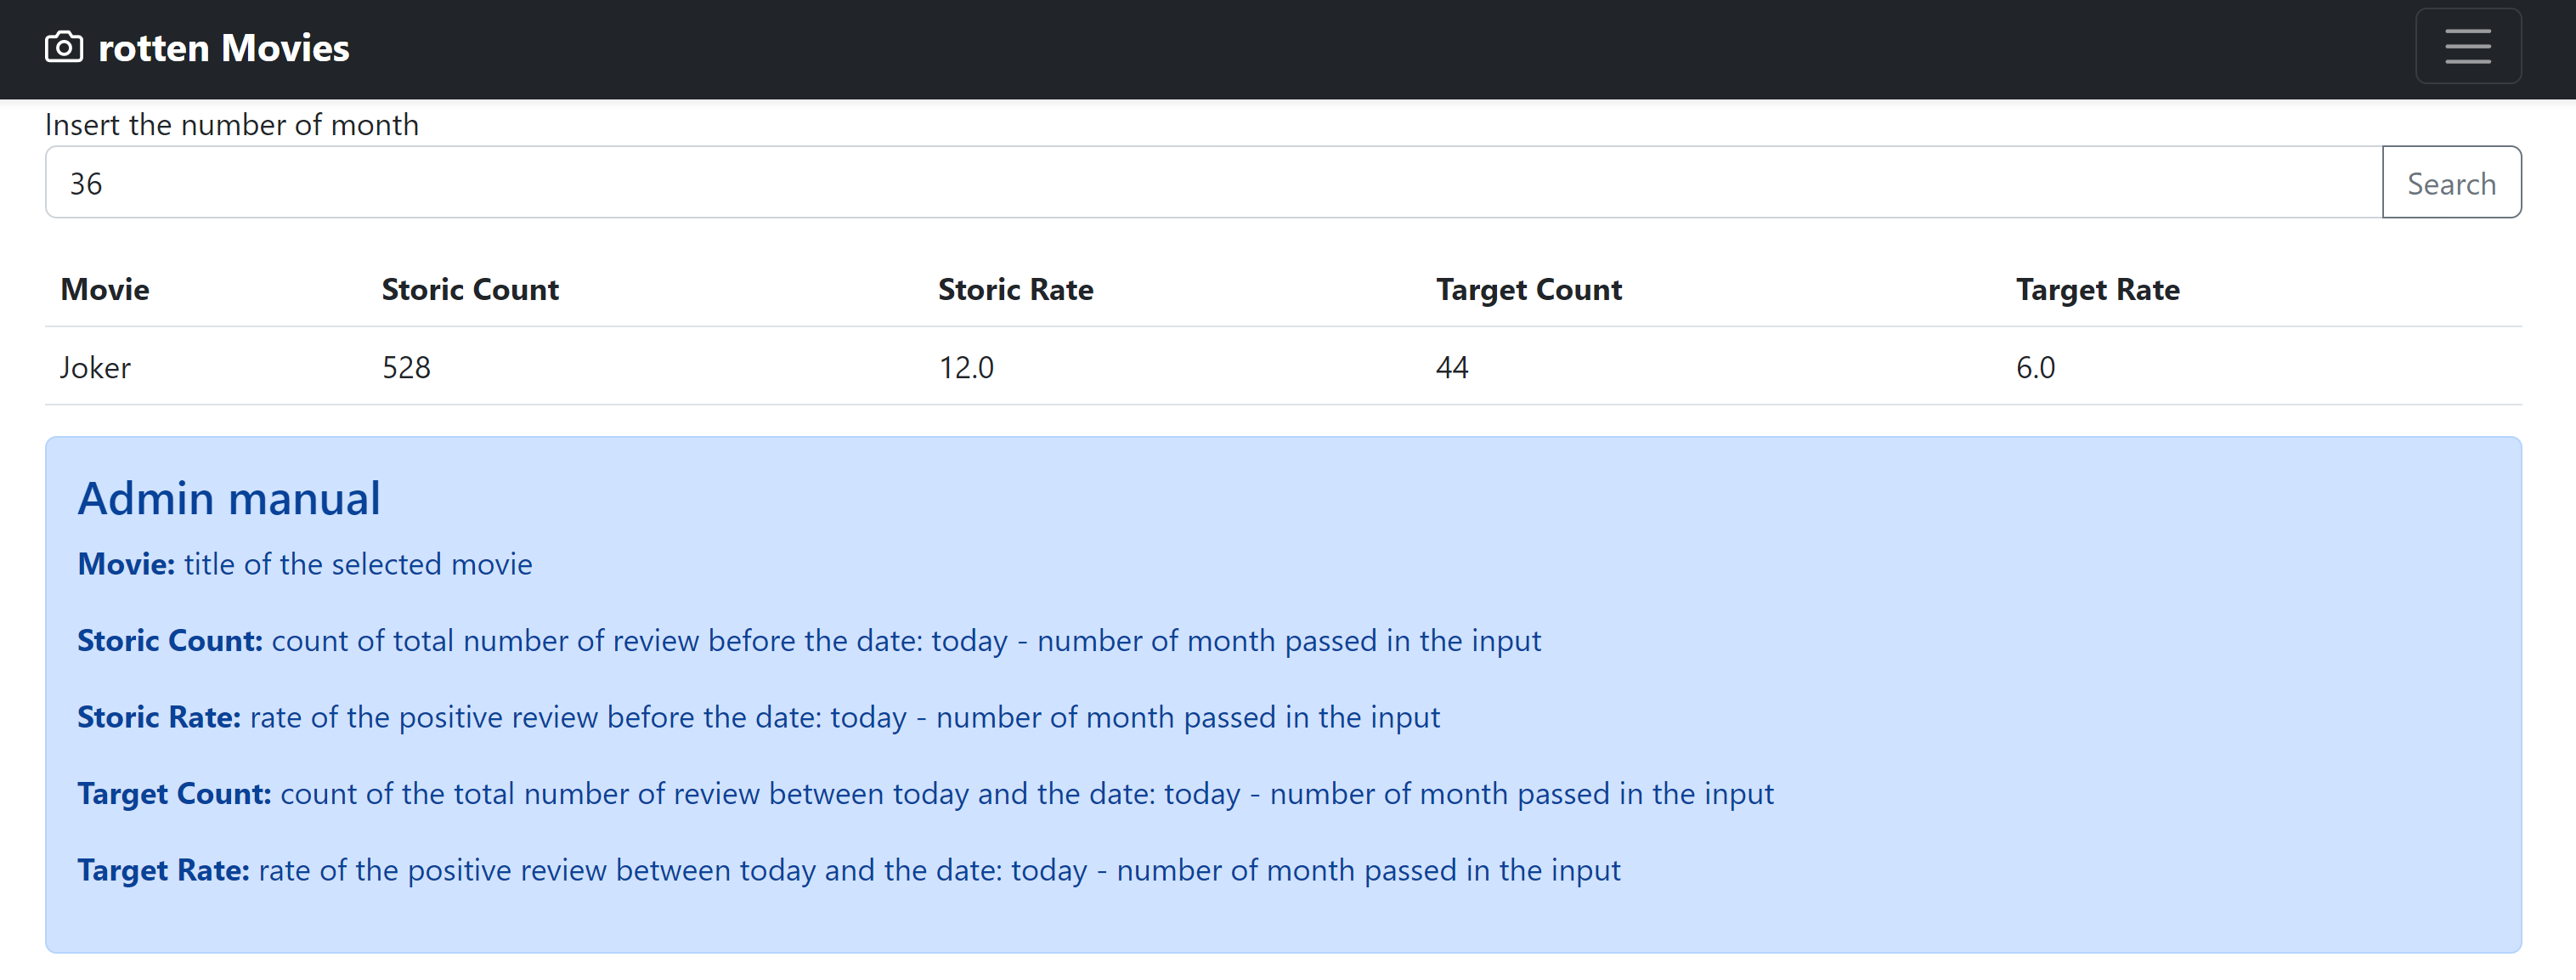
\includegraphics[scale=0.45]{../../../images/user_manual/review_bombing_page.png} 

\end{center}
\vspace{5pt}
The review bombing page shows some statistics about recent reviews made on a specific movie. An info box explains the meaning of each value


%\end{document}